%%%%%%%%%%%%%%%%%%%%%%%%%%%%%%%%%%%%%%%%%%%%%%%%%%%%%%%%%%%%%%%%%
%                          Packages                             %
%%%%%%%%%%%%%%%%%%%%%%%%%%%%%%%%%%%%%%%%%%%%%%%%%%%%%%%%%%%%%%%%%
\documentclass[a4paper,11pt]{report}
\usepackage[utf8]{inputenc}
\usepackage[a4paper, top=3cm, bottom=3cm, left=2.5cm, right=2.5cm, marginparwidth=2cm, headsep=1.2cm]{geometry} % layout
\usepackage[pdfencoding=auto]{hyperref} % enables hyperlinks in the PDF
\hypersetup{colorlinks=true, linkcolor=black, urlcolor=blue, citecolor=black} \urlstyle{same}
\usepackage{amsmath}
\usepackage{longtable}
\usepackage{cleveref} \Crefformat{figure}{#2Fig.~#1#3} % makes referencing customizable (e.g. \Cref{}). See: https://texblog.org/2013/05/06/cleveref-a-clever-way-to-reference-in-latex/)
\usepackage[nottoc, notlof, notlot]{tocbibind}  % includes bibliography in table of contents (TOC)
\usepackage[numbers]{natbib} % sets reference style
\usepackage{graphicx} % required to include images
\usepackage[svgnames]{xcolor}
\usepackage{tikz}

\usepackage{pgfplots}
\pgfplotsset{compat=1.17}

\usepackage{subfig}
\usepackage{siunitx} % makes it easier to use units (e.g. \SI{15}{mm}). See: https://mirror.foobar.to/CTAN/macros/latex/contrib/siunitx/siunitx.pdf
\usepackage[font=small]{caption} % reduces the caption's font size
\usepackage{eso-pic} % required to add the titlepage background image
\usepackage{lipsum} % To generate lorem ipsum dummy text
\usepackage{pgfgantt} % For Gantt chart creation
\usepackage{fancyhdr} % Changes the header & footer style
\usepackage{float}
\usepackage{bm}
\usepackage{amsfonts} 
\usepackage{booktabs}
\usepackage{multirow}
\usepackage{listings}
\usepackage{listings-golang}
\usepackage{adjustbox}
\usepackage{multicol}
\usepackage{glossaries}

\makeglossaries

\newglossaryentry{chair}
{
        name=Chair,
        description={Elected leader of the agents}
}
\newglossaryentry{manifesto}
{
        name=Manifesto,
        description={Conditions with which agents run for election as Chair}
}
\newglossaryentry{fight proposal}
{
        name=Fight Proposal,
        description={A list of thresholds to determine an agents fight decision}
}
\newglossaryentry{loot}
{
        name=Loot,
        description={Equipment dropped by defeated enemies, including swords, shields, health potions and stamina potions}
}
\newglossaryentry{potions}
{
        name=Potions,
        description={Drank by agents to restore health points or stamina points}
}
\newglossaryentry{bonus attack}
{
        name=Bonus Attack,
        description={Value of a sword equiped by an agent}
}
\newglossaryentry{bonus defense}
{
        name=Bonus Defense,
        description={Value of a shield equiped by an agent}
}
\newglossaryentry{common pool resource}
{
        name=Common Pool Resource,
        description={Loot dropped my enemy to be distributed amoungst agents}
}
\newglossaryentry{institutionalised power}
{
        name=Institutionalised Power,
        description={the power wielded by the Chair to control agents and direct their behavior through the use of rewards and punishments}
}
\newglossaryentry{sanctions}
{
        name=Sanctions,
        description={Methods by which the Chair punishes disobedience}
}
\newglossaryentry{alternative dispute resolution}
{
        name=Alternative Dispute Resolution,
        description={Settling disputes outside of formal proceedings with the assistance of an impartial dispute resolution body}
}
\newglossaryentry{social capital}
{
        name=Social Capital,
        description={Social value calculated by an agent and assigned to another}
}
\newglossaryentry{utility}
{
        name=Utility,
        description={Value of worth to the community or self, defined by an agent and assigned to another}
}


\lstset{
  language=golang,
  showstringspaces=false,
  columns=flexible,
  basicstyle={\small\ttfamily},
  numbers=none,
  numberstyle=\tiny\color{mygray},
  keywordstyle=\color{blue},
  commentstyle=\color{mygreen},
  stringstyle=\color{mymauve},
  breakatwhitespace=true,
  tabsize=4
}

\usepackage[ruled,vlined,linesnumbered]{algorithm2e}

\usepackage{placeins}
\usepackage{enumitem} % for enumerated lists other than 1. 2. 3. 
\usepackage{algpseudocode}

%%%%%%%%%%%%%%%%%%%%%%%%%%%%%%%%%%%%%%%%%%%%%%%%%%%%%%%%%%%%%%%%%
%                          Commands                             %
%%%%%%%%%%%%%%%%%%%%%%%%%%%%%%%%%%%%%%%%%%%%%%%%%%%%%%%%%%%%%%%%%
% Author
% Use \\ to separate multiple authors (e.g. Robert\\Nathalie\\Mike)
\newcommand{\myName}{SOMAS Class 2022}

% Title
% Introduce line breaks with \\
\newcommand{\myTitle}{Self-Organising Multi-Agent Systems}

% Type of Thesis
\newcommand{\thesisType}{Final Report}

% Date
\newcommand{\myDate}{December 2022}

% Supervisors
% Use \\ to separate multiple supervisors (e.g. Robert\\Nathalie\\Mike)
% Use full titles (e.g. Prof. Dr., Dr. )
\newcommand{\supervisors}{Prof.\ Jeremy Pitt}

% ToDo Command
\newcommand{\ToDo}[1]{\textcolor{red}{#1}}

%%%%%%%%%%%%%%%%%%%%%%%%%%%%%%%%%%%%%%%%%%%%%%%%%%%%%%%%%%%%%%%%%
%                          Page Format                          %
%%%%%%%%%%%%%%%%%%%%%%%%%%%%%%%%%%%%%%%%%%%%%%%%%%%%%%%%%%%%%%%%%

% Paragraphs
\setlength\parindent{0pt}
\setlength{\parskip}{2mm}

% Section Format
\usepackage[explicit]{titlesec}

%%%%%%%%%%%%%%%%%%%%%%%%%%%%%%%%%%%%%%%%%%%%%%%%%%%%%%%%%%%%%%%%%
%                        Title Page                             %
%%%%%%%%%%%%%%%%%%%%%%%%%%%%%%%%%%%%%%%%%%%%%%%%%%%%%%%%%%%%%%%%%
% Don't change anything here
\begin{document}
\begin{titlepage}
\newgeometry{top=2cm, bottom=4cm, right=1.5cm, left=1cm}

\tikz[remember picture,overlay] \node[opacity=1,inner sep=0pt, anchor=west] (A) at (2cm,-1.5cm){
\includegraphics[scale=0.5]{template_figures/logo.eps}};

    \begin{center}
        \vspace*{6cm}
        \huge \textbf{\thesisType}\\
        \vspace*{0.75cm}
        \Huge \myTitle\\
        \vspace{0.5cm}
        \Large {Department of Electrical and Electronic Engineering}\\
        \Large {Imperial College London}\\
        \vspace*{5cm}
        \huge \myName\\
        \vspace*{0.5cm}
        \LARGE \myDate\\
        \vfill
        Lecturer\\
        \vspace*{0.5cm}
        \huge \supervisors\end{center}

\end{titlepage}

%%%%%%%%%%%%%%%%%%%%%%%%%%%%%%%%%%%%%%%%%%%%%%%%%%%%%%%%%%%%%%%%%
%               Abstract & Table of Contents                    %
%%%%%%%%%%%%%%%%%%%%%%%%%%%%%%%%%%%%%%%%%%%%%%%%%%%%%%%%%%%%%%%%%
\pagenumbering{roman}

\begin{abstract}
Co-operative survival games refer to a subset of political choice games wherein `players' must work together to overcome disaster, else suffer the consequences through both personal and communal damage. Furthermore, without the ability to monitor a system and in the absence of a centralised authority, it becomes impossible to form enduring self-governing institutions, resulting in the proposed self-organising mechanisms for `solving' such games potentially functioning in harmful ways. This project utilises a self-organising, multi-agent system to simulate an iterated collective action, co-operative survival game comprising a resource management problem, the `solution' to which involves a system of localised governance. Through a series of experiments where the behaviour of the players in the system is increasingly randomised and the presence of self-organising mechanisms is toggled, we investigate the causes of instability. Ultimately, we conclude that through the integration of governance using treaties, it is possible for such a system to effectively self-organise to minimise the total deaths of the players involved.
\end{abstract}

\newpage
\tableofcontents
\newpage
\listoffigures
\newpage
\listoftables
\newpage

%%%%%%%%%%%%%%%%%%%%%%%%%%%%%%%%%%%%%%%%%%%%%%%%%%%%%%%%%%%%%%%%%
%                 Glossary & List of Symbols                    %
%%%%%%%%%%%%%%%%%%%%%%%%%%%%%%%%%%%%%%%%%%%%%%%%%%%%%%%%%%%%%%%%%

\section*{List Of Symbols}

\begin{description}

\item[\parbox{1.25 in}{$\delta$}] Range Modifier
\item[\parbox{1.25 in}{$\gamma$}] Hit Point Modifier 
\item[\parbox{1.25 in}{$\sigma$}] Linear Modifier
\item[\parbox{1.25 in}{$X$}] Enemy Resilience 
\item[\parbox{1.25 in}{$Y$}] Enemy Damage
\item[\parbox{1.25 in}{$HP$}] Health Points
\item[\parbox{1.25 in}{$ST$}] Stamina Points
\item[\parbox{1.25 in}{$c$}] Current Level
\item[\parbox{1.25 in}{$L$}] Total Number Of Levels
\item[\parbox{1.25 in}{$N$}] Number Of Agents  
\item[\parbox{1.25 in}{$\mu$}] Threshold Percentage 
\item[\parbox{1.25 in}{$M$}] Number Of Agents Required To Win game
\item[\parbox{1.25 in}{$N_f$}] Number Of Fighting Agents 
\item[\parbox{1.25 in}{$N_c$}] Number Of Cowering Agents 
\item[\parbox{1.25 in}{$HP_{pool}$}] Health pool
\item[\parbox{1.25 in}{$ST_{cower}$}] Cower Stamina Regeneration
\item[\parbox{1.25 in}{$HP_{cower}$}] Cower Health Regeneration   
\item[\parbox{1.25 in}{$A_s$}] Attack Base 
\item[\parbox{1.25 in}{$A_b$}] Attack Bonus
\item[\parbox{1.25 in}{$A$}] Attack Total  
\item[\parbox{1.25 in}{$D_s$}] Defense Base   
\item[\parbox{1.25 in}{$D_b$}] Defense Bonus
\item[\parbox{1.25 in}{$D$}] Defense Total
\item[\parbox{1.25 in}{$P_hp$}] Health Potion Value
\item[\parbox{1.25 in}{$P_st$}] Stealth Potion Value 
\item[\parbox{1.25 in}{$P$}] Potion Drop Quantity Percentage
\item[\parbox{1.25 in}{$E$}] Weapon Drop Quantity Percentage
\item[\parbox{1.25 in}{$N_p$}] Number Of Potions Dropped
\item[\parbox{1.25 in}{$N_e$}] Number Of Weapons Dropped
\item[\parbox{1.25 in}{$N_hp$}] Number Of Health Potions Dropped
\item[\parbox{1.25 in}{$N_st$}] Number Of Stamina Potions Dropped
\item[\parbox{1.25 in}{$N_a$}] Number Of Swords Dropped
\item[\parbox{1.25 in}{$N_d$}] Number Of Shields Dropped


\end{description}

\newpage
\printglossary
\newpage

\pagenumbering{arabic}

%%%%%%%%%%%%%%%%%%%%%%%%%%%%%%%%%%%%%%%%%%%%%%%%%%%%%%%%%%%%%%%%%
%                      Document Start                           %
%%%%%%%%%%%%%%%%%%%%%%%%%%%%%%%%%%%%%%%%%%%%%%%%%%%%%%%%%%%%%%%%%

\chapter{Introduction}\label{introduction}

\section{Introduction}\label{sec:intro}

% short introdcution to the module and the objectives/goals of the SOMAS cohort. 
% Some background on Self-Organising Multi-Agent System and its facets
% Ostrom Principals 
% Institutionalised power
% Game theory and strategic interaction 
% Social Choice Theory 
% alternative Dispute Resolution 
% Computational Justice
% Knowledge Agreggation 
% Sanctions and Dissent 

% outline of the report 
This report will present the definition of the game and design considerations that took place and the main objectives. The breakdown of the teams that were created, their members, responsibilities and work flows will be detiailed before presenting the implementations required to complete our objectives. Next the game design, DevOps and infrastructure work will be detailed to provide a thourough understanding of the game and its dynamics before agent teams present their strategies, algorithms and implementations. Experiemntal design results will procede a discussion on the implications of these results with respect to self-organising multi-agent systems. Finally there will be a short conclusion and reccomendations for future work will be outlined. 

\subsection{Story Line}\label{sec:story line}

% story line
For the implemented game, the following story-line was created: A rag-tag group of rebel peasants find themsevles at the bottom of a deep and dark pit. To escape to freedom, the peasants must battle through each rising level of the pit, slaying a number of perilous beasts on their way. With each enemy slayed at the blood soaked hands of the proletarian, they gain access to new and improved weaponry to fight on and never surrender. Once free, the peasants can continue their struggle against the totalitarian dictatorships of the western world, until, in God's good time, the New World, with all its power and might, steps forth to the rescue and the liberation of the old.  

To achieve all these goals, peasants must self-organise to survive. This can be done by electing governors, conducting collective risk analysis, assigning common pool resources and performing alternative dispute resolution using institutionalised power. All of these aspects, revolve around the understanding of social choice theory and knowledge agreggation. 


\subsection{Rules, Attributes \& Artifacts}\label{sec:rules}

The objective of the game is for an Agent to win, individually, by escaping the pit with as many `hit-points' and `health points' as possible, whilst also ensuring that enough of your fellow players survive to start the revolution upon esape. 
For each level within the pit, combat consists of a number of fight rounds which continue until either; the enemy is defeated, or the agents turned into chutney. Within each round, Agents can either; attack, defend, or cower. The first action deals damage to the enemy, the second absorbs damage from the enemy, and the final option skips the round whilst regenerating health and stamina.
Agents will be granted multiple opportunities within fight rounds and pit levels to self-organise. These self-organisational tasks could involve the allocation of loot dropped by a vanquished foe. This perticular example occurs at the end of each fight, before advancing to the next level of the pit. Expansion and explination of each of the task will be introduced later in this report. 

Before listing the rules of the games, it is important to give a simple overview of the Agent and enemy attributes as well as the equipment that can be used within the game.  

\subsubsection{Attributes \& Equipment}

All Agents within the game have the following attributes:

\begin{itemize} 
    \item Health Points ($HP$)
    \item Stamina Points ($ST$)
    \item Attack Base ($A_s$)
    \item Attack Bonus ($A_b$)
    \item Defense Base ($D_s$)
    \item Defense Bonus ($D_b$)
\end{itemize}

Attack and defense bonuses represent the value of the equipment that is currently being used by the agent. The base values are native to all agents and remain contant, the minimum fight potential of an agent. For the enemy's attributes:

\begin{itemize}
    \item Resilience ($X$)
    \item Damage ($Y$)
\end{itemize}

Equipment is divided into two sections, weapons and potions. Each weapon is of a specific hit value and can be equiped by an Agent to increase their damage (or shield) potential. There are only two weapon choices:

\begin{itemize}
    \item Sword ($A_b$)
    \item Shield ($D_b$)
\end{itemize}

Swords are used by Agents who attack, and shields are used by Agents who defend. In both cases, their potential would be the conbination of both base and bonus attribute values, giving the Total Attack (/Defend). Potions are consumed by Agents to regenerate their attributes, specifically $HP$ and $ST$. Again, there is a specific value assigned to each new potion. 

\begin{itemize}
    \item Health Potion ($P_{hp}$)
    \item Stamina Potion ($P_{st}$)
\end{itemize}

The value mechanisms for all these variables will be outlined in Section. ADD MATHS SECTION NUMBER. 

\subsubsection{Rules}
Now that the basic game variables have been defined, the standard rules of the game can be listed. 

\begin{enumerate}
    \item All agents start with equal $ST$, $HP$
    \item An enemy dies if $\sum_{i} (A_b_i + A_s_i) > X_{remaining}$ at the end of a round
    \item Damage dealt to agents who fight = $\gamma Y - \sum_{i} (D_bi + D_si)$ 
    \item An agent dies if $\frac{\gamma Y - \sum_{i} (D_bi + D_si)}{N} > HP$
    \item To attack: $ST \geq (A_b + A_s)$
    \item To defend: $ST \geq (D_b + D_s)$
    \item If an agent attacks, $ST -= (A_b + A_s)$
    \item If an agent defends, $ST -= (D_b + D_s)$
    \item If an agent cowers, $HP += HP_c$, $ST += ST_c$
    \item If all agents cower, all recieve damage $\gamma Y$
    \item If, at the end of a round, $N<M$, the game ends 

    \item Agent can hold extra equipment in their inventory
    \item Agents can donate $HP$ to the $HP_{pool}$ at the end of each level
    \item If $HP_{pool} > X$, agents pass level without fighting

    \item Before each round, agents may communicate to decide fight actions and Chairs may issue sanctions to those to defected from the group strategy (if they wish)
    \item At the end of each level, agents may communicate to allocate the common resource pool, elect new governments, trade equipment and resolve any disputes.


\end{enumerate}

% Agent / Enemy Attributes and variables 
% specifications and Rules
% standard rules

Besides these standard rules, there were a number of additions that were made. To add new dimentions to the game's social ascept, agents only have access to granulated views of their fellow agents $HP$ and $ST$ attributes. This addition creates a high degree of uncertainty in agent calcualtions and inferences which could create interesting outcomes or large changes in group fight decisions. An agents inventory will be private, allowing agents to hoard equipment without others knowing. This too allows a higher range of agent strategies and introductes more oportunities for selfishness and exploitation. 

Fight decision strategies are proposed for the whole group and chosen once a majority has been achieved. Deviation from this aggreed strategy can result in sanctions, determined by the Chair. Sanctions can include being forced to fight for a set number of rounds with zero fight attributes. Potential chairs must run for office on a number of policies and are chosen by plurality during governance elections. Finally, an disputes are resolved by the Chairs individual ideals or by the games determination of group utility. All of these decisions attempt to add the concepts of institutionalised power and social choice theory to the game. The specific mechanisms of collective actions and governance will be further detailed in Section.GAME DESIGN.

% more nuanced rules and the reasons for these rules 

\subsection{Aims \& Objectives}\label{sec:aims}

The overarching objective of this project was to test the self-organisational skills of independent agents when placed into a survival, multi-agent environment. We desired to examine the creation and degredation of relationships between agents based on differing ideolegies and whether those relationships are based on facets such as; trust, expertice, community contribution or social capital. Another aim was to explore the different types of governments that would be formed by these agents to determine which governance strategy produced the best results, and which caused the most unrest. Further exploration of the range and severity of sanctions placed upon disobedient agents within an unhappy community would complement the evaluation of a Chairs effectivness to rule. Finally, we attempted to witness the effect of scaling the number of agents within the game on the groups ability to escape the pit and do so as a community. 

For individual agent teams, the objective was to escape the pit whilst achieving the highest utility to the community and the highest utility to the self. When analysis the result of any experimental design, we aim to propose the best agent strategies and the most effective impementation to acheive this strategy, with respect to implementation algorithms. 

An anxially aim was to assess the effectiveness of our own self-organisation when attempting to achieve these goals. To outline areas of short falling or efficieny and suggest possible improvements that would have led to more efficient work-flows and agents that could defeat more difficult versions of the game. 

As a final objective, we wanted to develop a metric capable of quantifying an agents utility to the group and therefore define a `winner' of the game. 
% enter the aims of the game 
% to test the self-organisational skills of multiple independently designed agents within the game
% to experiemnt with the group of agents and see weather they form relationships based on trust, expertise and community contribution 
% to test the effectiveness of any governments established by the agents, the levels of defections from the group strategy and the severity of any sanctions that are applied. 
% finally to see if scaling the number of agents influences the effectiveness of said governments and the communities progression through the game. 

% finally to attempt to indentify a winner of the game. The definition of the `winner' will be explored in Section.GAMEDESIGN. 


\subsection{Team Structure}\label{sec:team struct}

To accomplish the goals that have been defined in the previous sub-section, we self-organised into 6 `Agent Teams'. Each team is reponsible for implementing their own agent, with their own ideologies and intuitions of how social interactions, coupled with knowledge aggregation, can be utilised to obtain high levels of game proficiency. They will also be in charge of documenting their progress and ultimatley writing a report detailing their implementation strategy and experimental design results. Finally, teams must provide code reviews for other teams to maintain consistency of standards and practices. The agent teams, and their members, are defined in \Cref{fig:agentteams}. Team leaders impose some hierachey, and will represent the teams opinions on group decisions as well as updating people on their progress. Overall group decisions will then be decised via concensus of the team leaders. 

\begin{figure}[htb]
    \centering
    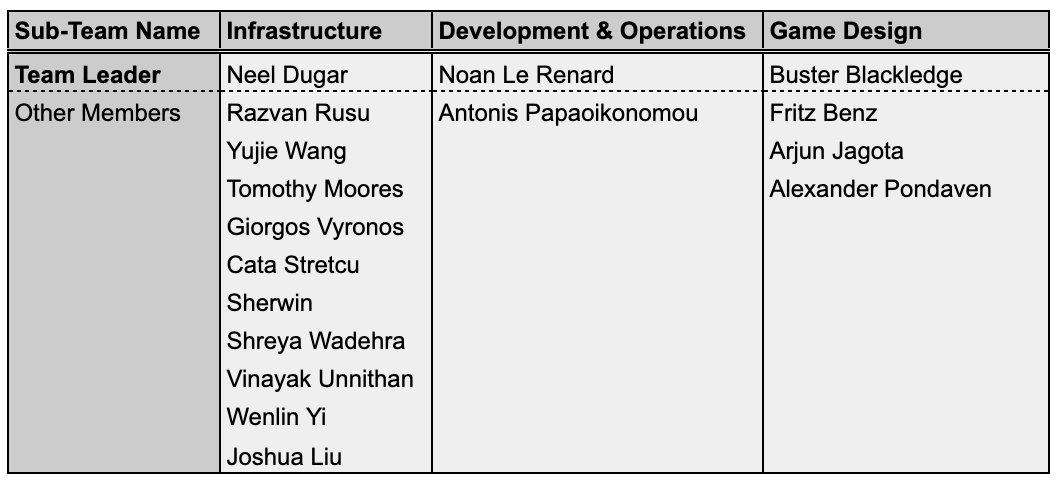
\includegraphics{000_introduction/images/agentteams.png}
    \caption{Breakdown of the agent teams, their team leaders and members}
    \label{fig:agentteams}
\end{figure}
    
Besides agent teans, there are a number of other sub-teams that are required to complete the project. All of these sub-teams will also be responsible for their output documentation, report section writing and providing regular updates to the group. 
The first is the infrastructure team, and will have the following responsibilities;

\begin{itemize}
    \item Game flow implementation
    \item Agent to server interface
    \item Agent communcication standardisation
    \item Front end implementation
\end{itemize}

A major responsibility of this team is the documentation of thier functions and methods so that agent teams can easily integrate their agent ideologies within the game. Their work will be exploared in detail in Section.INFRA

The next sub-team is Game Design, who have the following responsibilties;

\begin{itemize}
    \item Game variables alogrithmic definitions
    \item Game Machanism definitions 
\end{itemize}

Finally the Development and Operations sub-team was in charge of;

\begin{itemize}
    \item Maintaining version control \& work-flow
    \item Git actions
    \item Unit tests to ensure code integrity
    \item Deployment tools and scripts
\end{itemize}

Each one of these sub-teams was created by agent teams donating 1-2 of their members to each, the breakdown of each team is shown in \Cref{fig:subteams}.

\begin{figure}[htb]
    \centering
    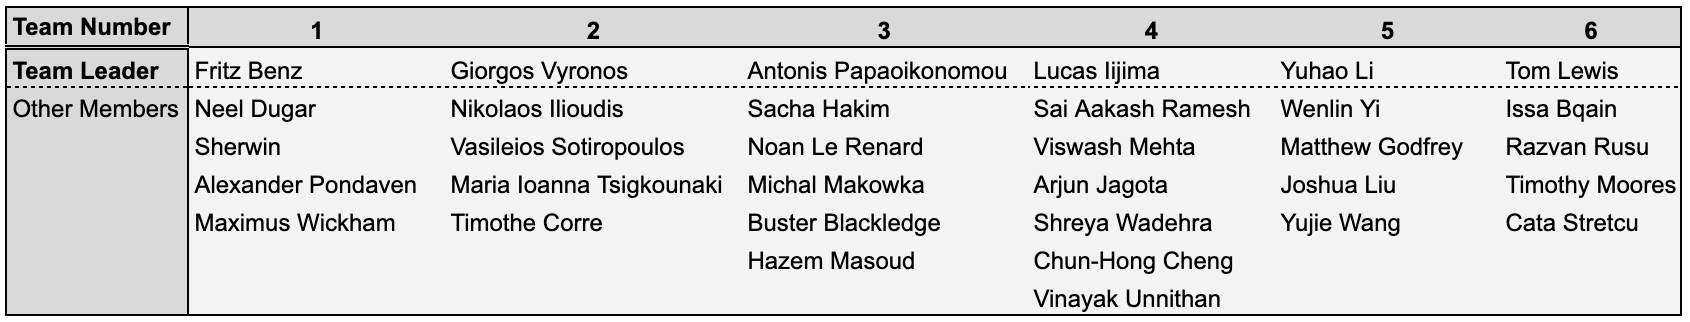
\includegraphics{000_introduction/images/subteams.png}
    \caption{Breakdown of the sub-teams, their team leaders and members}
    \label{fig:subteams}
\end{figure}

%% input the strucutre of each team
% how does the flow of each team work 
%% input each team and who is in each team 

Finally, the overall project was led by Buster Blackledge who was responsible for coordination. This structure was used in order to allow everyone to be involved in agent design, whilst allowing all agent teams to have direct access to at least a single member of the infrastructure team. 

As for the decision process. Team leader meetings would discuss design considerations, where each leader represents the opinions of their team members, and make decisions after a consensus had been reached. 



\chapter{Simulation Structure}\label{simulation_structure}
\chapter{Data Logging and Dashboard}\label{data_logging}
\chapter{Team 1 Agent Design}\label{team_1_agent_design}

\section{Overview}

The following chapter presents the design and implementation of Team 1's agent. The agent presented agent seeks to imitate important parts of human behaviour such as social status, social networks, selfishness, forgiveness and learning from experiences. At the end of the chapter, it will be shown that by using these concepts, the agent produces better collective outcomes over agents performing random actions.

\section{Core Structure}
Figure \ref{fig:agent_structure} presents a high-level overview of the structure and operation of our agent. In broad terms, the agent contains three elements which impact decision-making. These elements are:
\begin{enumerate}
  \item Social capital: Socially constructed resources which facilitate cooperation to solve collective problems.
  \item Selfishness: A continuously updated variable dictating to what degree an  agent prioritizes its own utility over the social welfare of the group when making decisions. 
  \item Q-functions: Functions learned through reinforcement learning which estimate the impact of actions given the current game state.
\end{enumerate}
In addition to these components which are inherent to the agent, the current state of the game, known as the \emph{environment}, also influences decisions. Exactly how each component is used in the decision making process varies between different types of decisions, and social capital, selfishness and q-functions are not all used for every decision. The specific decision process for each type of decision will be discussed in greater detail in \ref{}.

%However, a general decision flow can be as follows: The agent takes in the current game state and passes it through a set of Q-functions. The Q-functions return the expected utility of each action to the collective and to the agent itself. Based on its current selfishness value, the agent aggregates the two utility values into a single value for each action.   Generally, the decision flow 

After each round of the game, the agents will update their internal state. Specifically, the agents will update their selfishness based on the current environment and the social capital of agents, while the social capital will be updated based on the actions of agents. The social capital is also updated every time an agent receives a message from an agent in their network. All of these update mechanisms are indicated by red arrows in Figure \ref{fig:agent_structure}. As can be seen, there is no arrow feeding back to the Q-functions as they do not update over the course of a single game. Instead, the Q-functions are updated based on the results from a series of games. However, as will be discussed later, the updating of selfishness values does still permit the agents to learn from experiences during a game.

% In addition to selfishness and social capital the agent also maintains a set of state variables that are used to make decisions with regard to leadership and voting. The most important of these is a measure of how well each agent in currently doing. This variable has to take into account many different aspects of game state and can be fairly difficult to create as defining a good game position is not obvious and of course depends on the decisions of others. An example of this difficulty is in deciding whether or not an agent having a higher attack value suggests it is doing better, in this case we found this to be a bad thing as in makes the agent more likely to have to engage in fights compared to agents with lower attacks. Several different factors such as this were combined to form this single variable which will be referred to as agent survival likelihood from here on. Once this score was computed for each agent all the scores were scaled such that the maximum score was less than 1 and the minimum was greater that 0, in addition, the mean was shifted so as to be close to 0.5. Finally, the standard deviation of this data-set was computed to give an indication of the spread of agents states, as the variation in state across the population can be a big factor in agent decision making. 

\begin{figure}[!h]
    \centering
    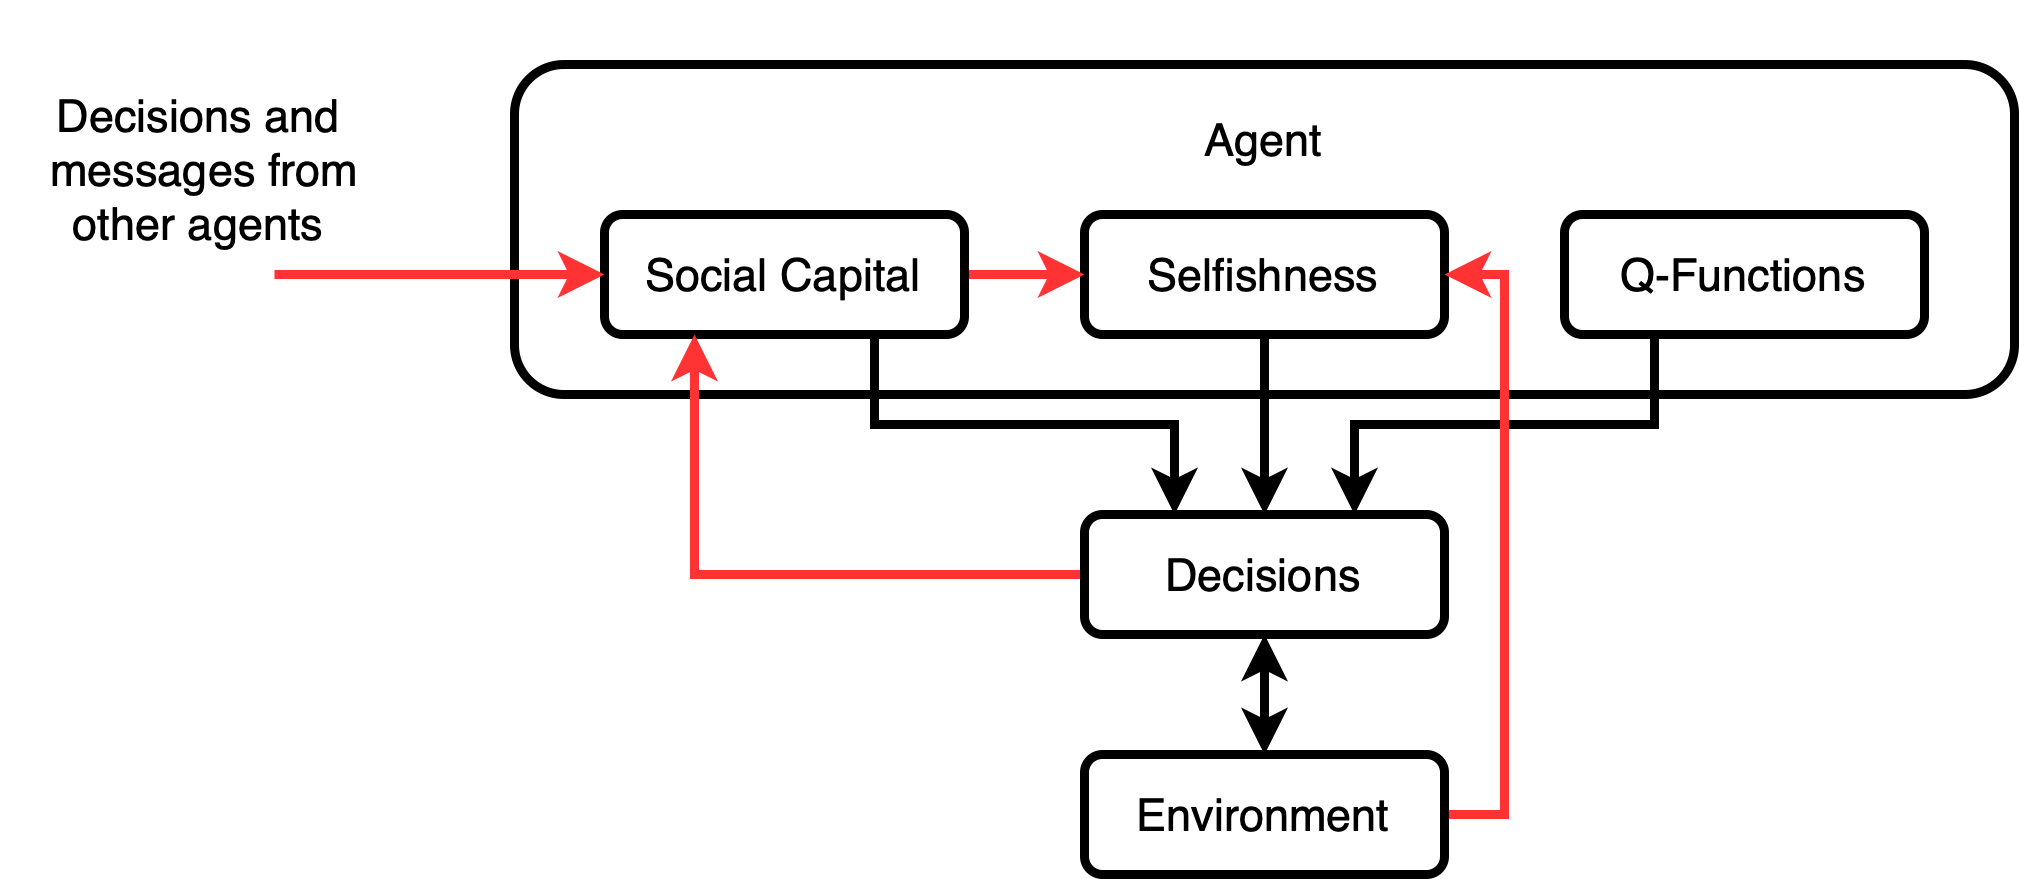
\includegraphics[width=0.75\linewidth]{004_team_1_agent_design/images/agent_structure.png}
    \caption{Overview of agent structure.}
    \label{fig:agent_structure}
\end{figure}

\section{Social Capital}

The core concept underlying the design of the agent is the idea of social capital. The exact definition of the term "social capital" varies between works, but can be summarized as "an 'umbrella term' for a range of socially constructed conceptual resources that help people coordinate expectations and self-organise."\cite{pitt}. Several forms of social capital have been identified and defined. Our work on social capital is mostly related to those forms laid out by Elinor Ostrom and T. K. Ahn in their 2007 paper "The meaning of social capital and its link to collective action". \cite{ostrom-ahn} In their paper, Ostrom and Ahn identified three forms of social capital. These were \emph{Institutions}, \emph{Networks} and \emph{Trustworthiness}. In addition to the forms of social capital presented by Ostrom and Ahn, we have as a team identified another form of social capital elected to call \emph{Honour}. With \emph{Honour} we refer to the human tendency to want to return a favour, or similarly, our appetite for revenge. A more comprehensive definition of honour is given in section \ref{subsection:honour}. 

In order to use social capital to promote cooperation, it must be used as part of a framework where the actions of an agent impact their social capital and where the social capital is used to make informed decision on whether or not to cooperate with other agents. For our agent, we used a similar framework to that presented by Petruzzi, Pitt, and Busquets\cite{complexity_reduction}. An overview diagram of this framework is presented in Figure \ref{fig:social_capital_framework}. In this framework events coming the environment are translated into social capital information which is passed to internal update functions for calculating metrics for each type of social capital. The social capital decision module uses the social capital metrics to calculate a value from 0 (no cooperation) to 1 (full cooperation) indicating whether an agent should cooperate or not. Implementing this framework for a simple cooperation game, Petruzzi et al. were able to achieve better performance than the dominant strategy given by game theory analysis. 

\begin{figure}[!h]
    \centering
    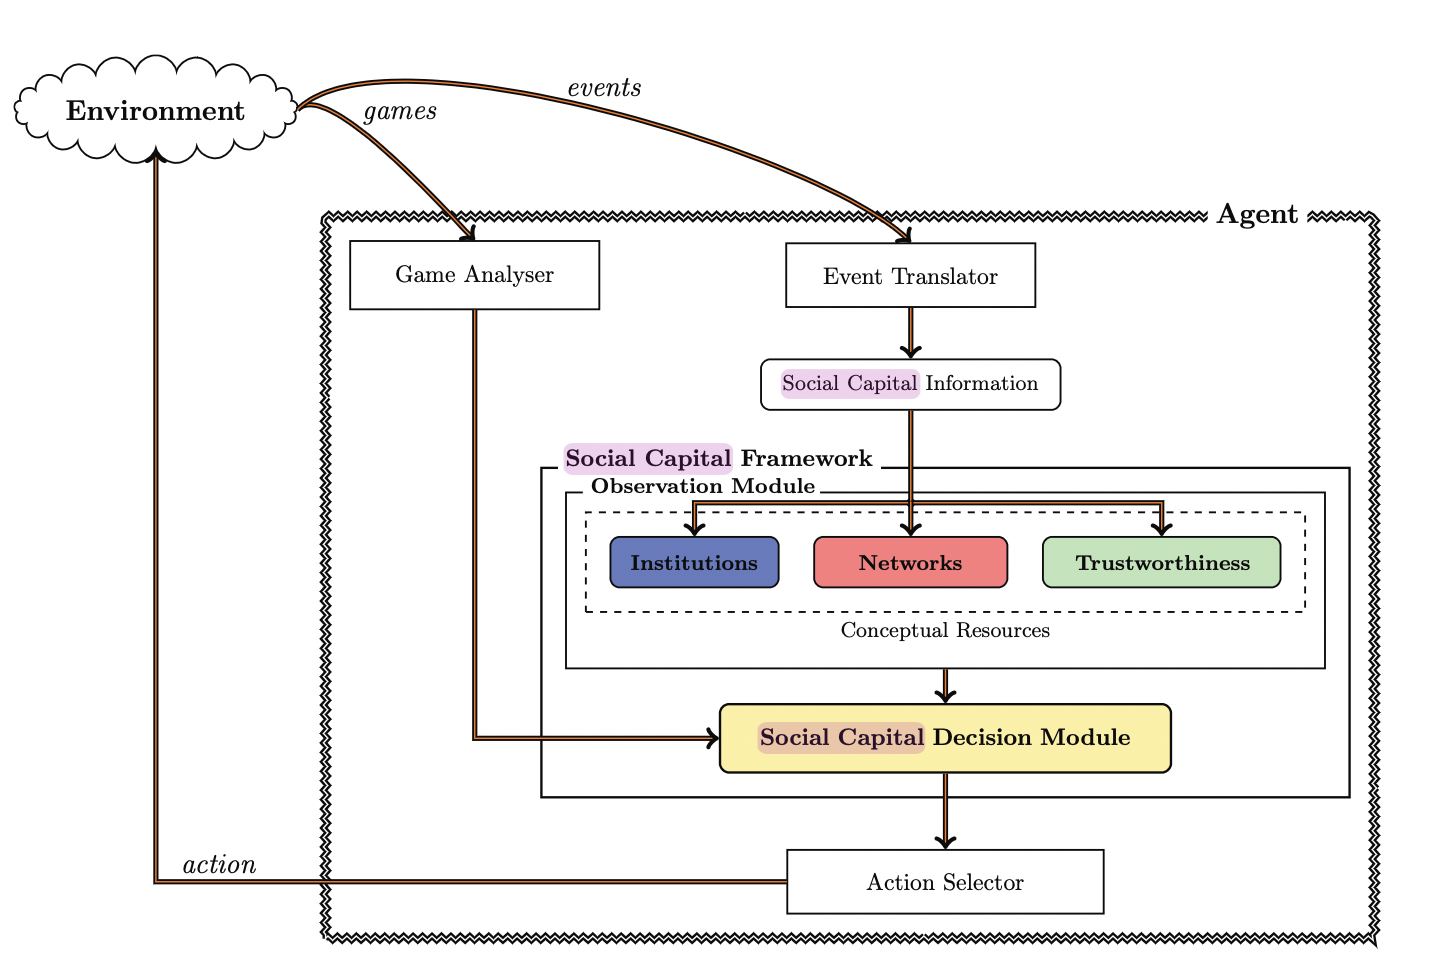
\includegraphics[width=0.75\linewidth]{004_team_1_agent_design/images/socialcapitalframework.png}
    \caption{Framework for a social capital system.\cite{pitt}}
    \label{fig:social_capital_framework}
\end{figure}

To apply the framework to the Escape the Dark Pit(t) game, we used a slightly different implementation than Petruzzi et al. used for their cooperation game. Most prominently, we simplified the stored metrics on social capital down to a single number between -1 and 1 for each form of social capital. We also simplified the social capital decision module by removing the possibility of weighting social capital indicators differently, reducing the decision module to a simple summing function. 

The specific implementation is as follows. Each agent has a member variable $socialCaptial$ which is a map between agent ids and an array with 4 values. From index 0 to index 3, this array holds values describing the social capital related to institutions, networks, trustworthiness and honour respectively for the agent with the specified agent id. Each agents $socialCapital$ map contains an array for every single agent in the game, including themselves. The array values are bounded between -1 and 1, where a higher number indicates higher social capital. When an agent is created, all the array values are initialized as 0. This is a neutral state in which no agent has a negative nor positive impression of another agent. Throughout the game the array values for each agent will change based on their actions and messages received about them. In general, if an agent does a non-cooperative actions the array values will decrease and become negative, and inversely cooperative actions will give positive array values. As such, agents will try to reward other agents for which their $socialCapital$ map indicates positive social capital and punish those who have negative social capital.

The following subsections go into detail regarding the implementation of each form of social capital.

\subsection{Institutions}

In their 2007 paper Ostrom and Ahn defined institutions as "prescriptions that specify what actions (or outcomes) are required, prohibited, or permitted, and the sanctions authorized if the rules are not followed" \cite{ostrom-ahn}. With our $Institutions$ social capital value we seek to provide a metric on how likely an agent is to follow these prescriptions and cooperate within institutions. 

During a game our agents place the following expectation on the interaction of other agents with institutions:

\begin{enumerate}
    \item If the leader makes a fight proposal, all agents should follow that proposal.
    \item If the leader makes a loot allocation proposal, all agents should follow that proposal.
\end{enumerate}

Failing to comply with any of these two expectations will lead to an agent being labelled as a defector. Once labelled as a defector, an agent's social capital value for institutions will for the rest of the game be given a base value of -1. As such, even deviating from the required action once will lead to a negative perception for the entirety of the remaining game. This is similar to a grim trigger strategy for cooperation. The reason why we elected to have defecting in even a single round negatively effect the social capital of an agent for all remaining rounds is due to the limitation on available information from the game. In its current version, the list of defectors which the game makes available to agent has the same type of static behaviour where defecting once will lead to an agent being labelled a defector for the rest of the game.

In order to increase their $Institutions$ social capital value agents must demonstrate their cooperation within institutions. For our agents there is just a single way of doing this: being elected leader. For as long as an agent is the leader, they will get a temporary boost of +1 to their $Institutions$ social capital value. Originally, agents tendency to sanction defectors was also planned to impact their social capital. In this case, doing actions which punish defectors such as voting against them in elections and not trading with them would yield positive social capital. Inversely, voting for defectors or trading with them would yield negative social capital. However, this was in practice found to be hard to implement, and has been left as a possible future extension.

\subsection{Networks}
The $Networks$ social capital value is a measure of an agent's reputation among other agents. Specifically, the $Networks$ value tries to estimate the average social capital perception of the given agent among the other agents in the game. The network is also used by agents in order to determine which other agents they want to share social capital information with. This way, agents will form a social networks in which each agent is liked by the other agents in its network.

In our current configuration, an agent will communicate with other agents if they have a social capital $Networks$ value greater or equal to $T_{N_0} = 0.5$. Previously, we said that all social capital values are initialised to 0. This is however a slight simplification, as in reality we initialise a small subset of $Networks$ values for each agent to 0.8. This was necessary given the way an agent decides whether to communicate with other agents, as all 0 $Networks$ values would lead to agents never communicating and thus the $Networks$ values never updating. 

We investigated several ways of determining what $Networks$ values to give a non-zero initialization and thus which other agents an agent should communicate with from the beginning.

\begin{figure}[!h]
    \centering
    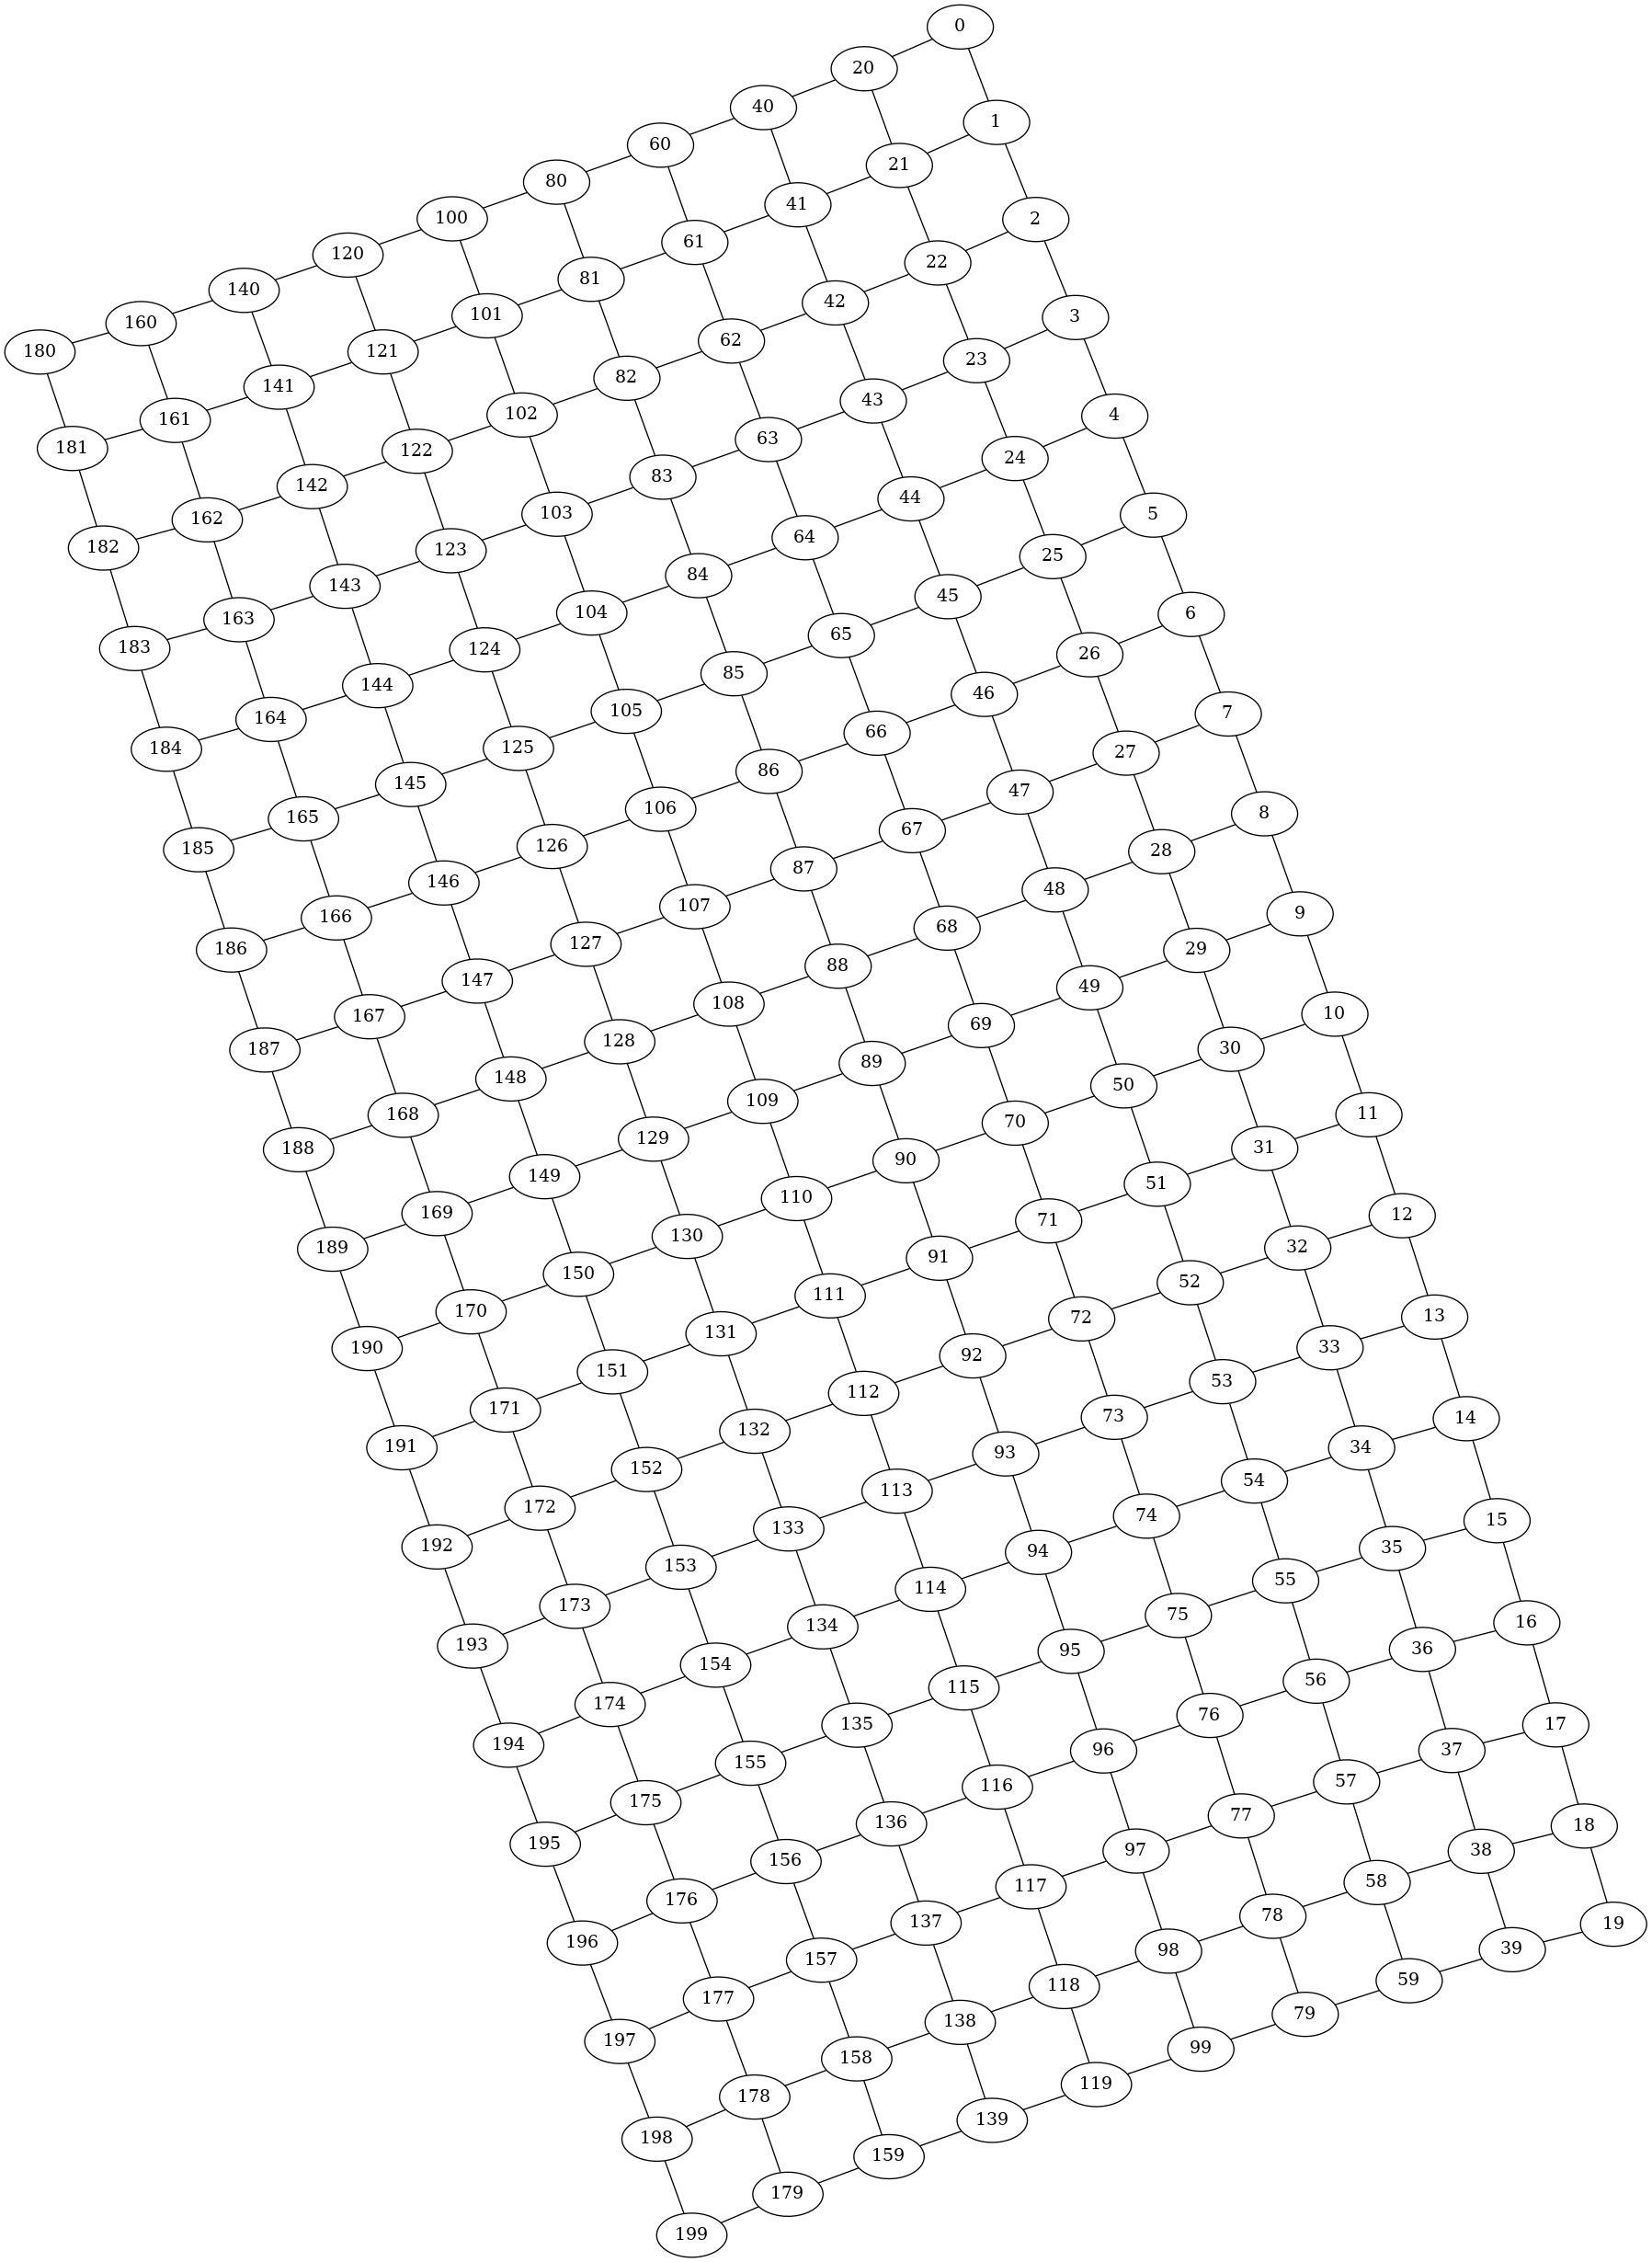
\includegraphics[width=0.4\linewidth]{004_team_1_agent_design/images/sc_network_grid.png}
    \caption{Grid initialisation of 200 agents}
    \label{fig:sc_network_grid}
\end{figure}

The network value of an agent can be initialised at the start of the game. For example, agents can be initialised in a grid structure (figure \ref{fig:sc_network_grid}) where most agents are connected to 4 other agents, aside from agents at the edges or corners that are only connected to 3 or 2 agents respectively.

\begin{figure}[!h]
    \centering
    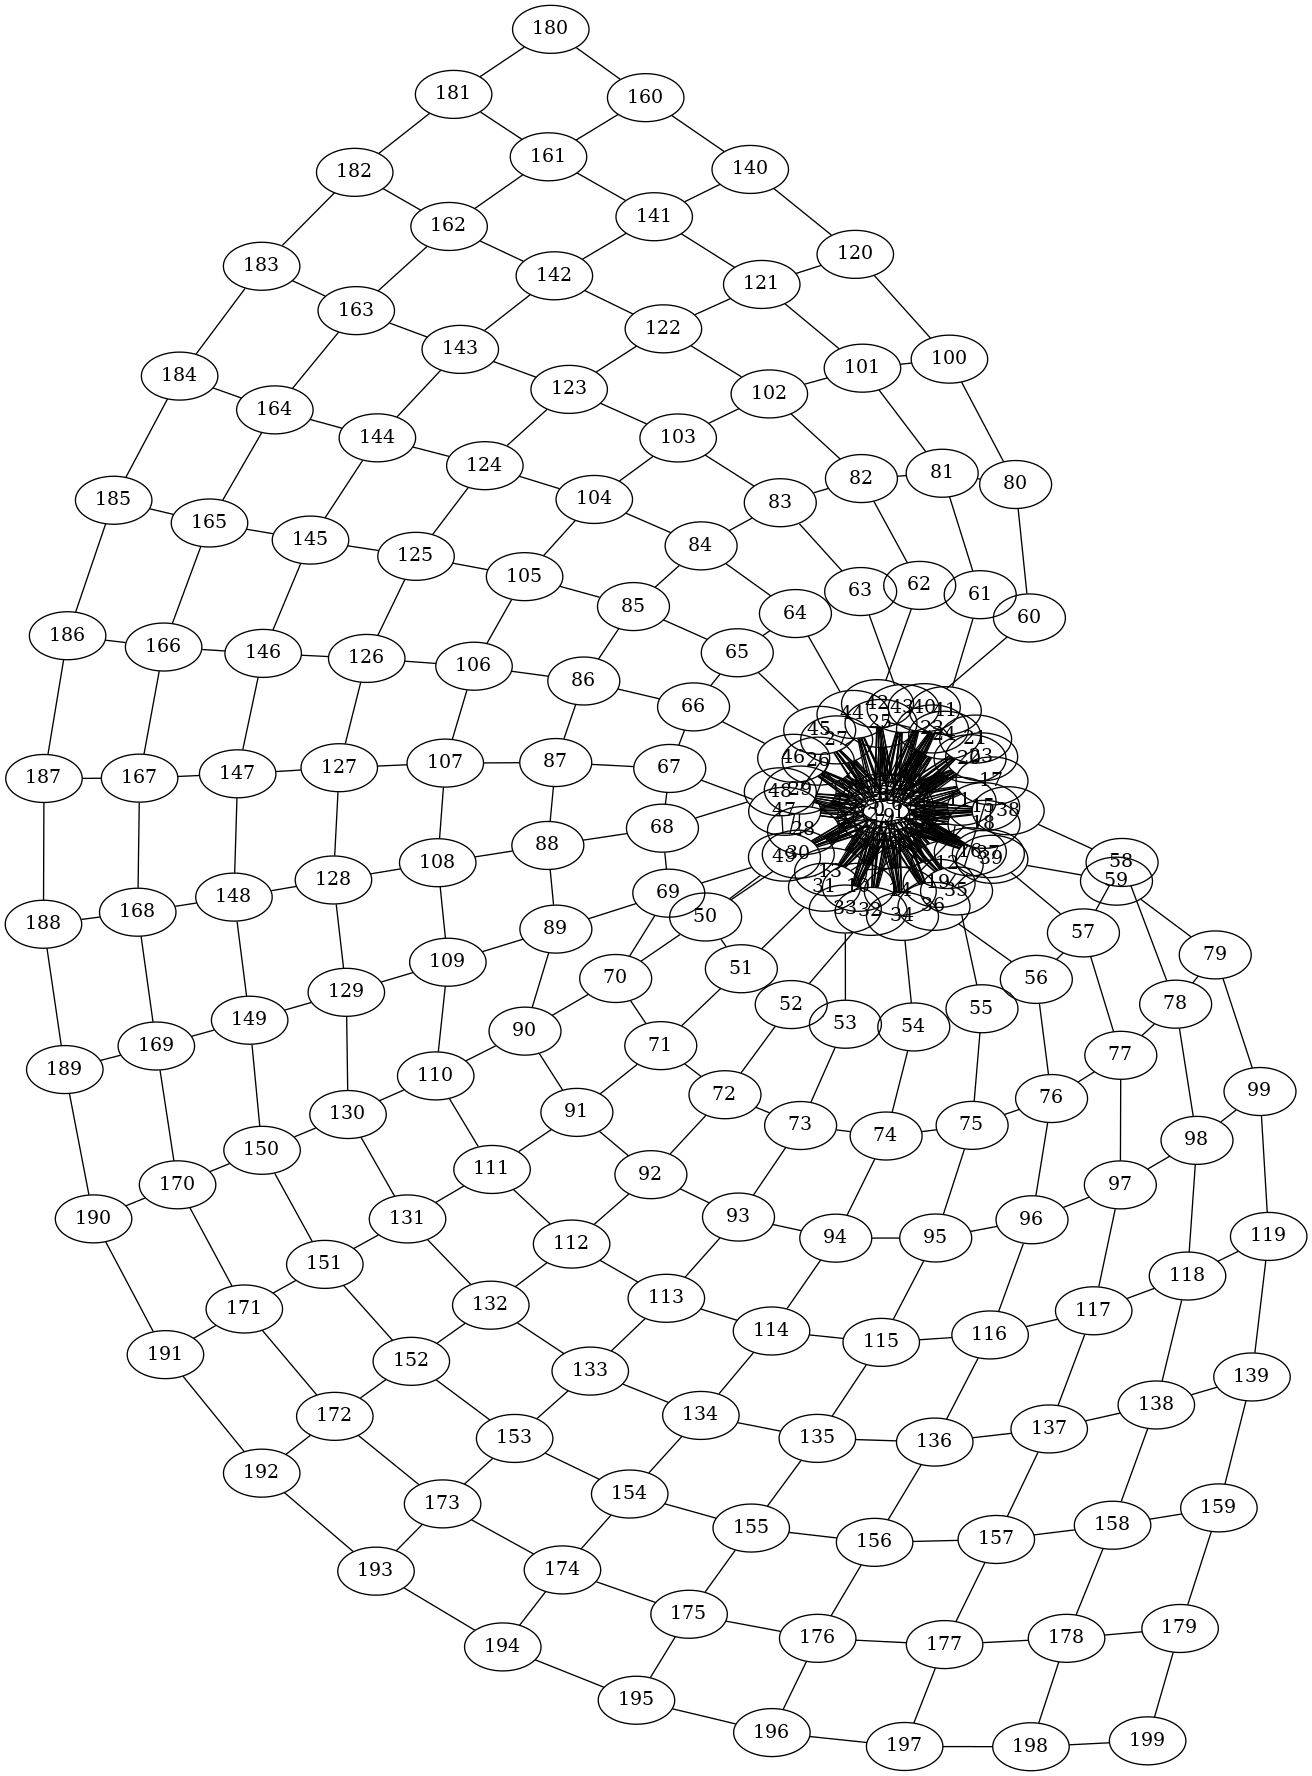
\includegraphics[width=0.4\linewidth]{004_team_1_agent_design/images/sc_network_clique.png}
    \caption{'Clique' initialisation of 200 agents}
    \label{fig:sc_network_clique}
\end{figure}

More complex initialisation patterns can also be explored. In this 'clique' initialisation pattern (figure \ref{fig:sc_network_clique}) the first 10 agents are all each connected to each other and 40 other agents. Consequently, those next 40 agents are each connected to the first 10 agents with a few connections to the rest of the grid, producing three tiers of agents with connections.

These network values can change during the game itself, and is updated as follows:
\begin{enumerate}
    \item At the start of each fight round, agents gossip to their connections about $N_A$ agents with the highest average Trustworthiness and Honor values - thereby praising them. The number of agents gossiped about in the message, $N_A$ is given by 
    \[
    N_A = P_A * (number of alive agents)
    \]
    where $P_A$ is the proportion of living agents admired (set to $0.1$) and $0 < P_A < 0.5$. A message is sent to the agent's connections containing a list of the agents and indicating that they are being praised.
    \item The same happens for agents with the lowest average Trustworthiness and Honour values, with a proportion of alive agents disliked (set to $0.1$) being denounced and 
    \item Upon receiving praise from an agent A about agent B, the agents network value of B increases, while the opposite is true if agent B was denounced. The network value of agent B changes based on the following formula:
    \[
    network_B += sign * perception_A * 0.1 * network_B
    \]
    
    Where $sign$ is $+1$ if the agent is praised and $-1$ if the agent is being denounced. $perception_A$ is the overall perception (average social capital value) of the sender. This means that if the sender has a negative social capital value then effect of the senders message is actually reversed.
% TODO: Update these once we twweak the calculations in the game
\end{enumerate}

In the above update stages agents do not praise or denounce themselves, though an agent may directly tell an other agent that they are praising or denouncing them through these messages.


\subsection{Trustworthiness}

In their 2007 paper Ostrom and Ahn give multiple examples of trustworthiness, but give no concise definition. One definition fitting the examples of Ostrom and Ahn is that given by Pitt in his 2021 book on Self-Organising Multi-Agent Systems: "Trustworthiness, as distinct from trust, and related to reputation, being a shared understanding of someone’s willingness to honour agreements and commitments"\cite{pitt}. In their paper, Ostrom and Ahn treat trustworthiness as a function of an individuals observable characteristics such as appearance, dress, gender, age and language. Moreover, they give examples of so called "one-shot" situations in which an individual has to decide on whether to trust another individual which they have never previously interacted with.\cite{ostrom-ahn}

Given that agents' interactions in the Escaping the Dark Pit(t) game are not one-shot, but repeated, handling trustworthiness as an inherent property of an agent's current observable characteristic is not ideal. Instead, as agents interact many times, it is more natural to use previous interactions to estimate future cooperativeness. Our agent therefore does not use observable characteristics to determine trustworthiness, as Ostrom and Ahn did. Instead, we define an agent's trustworthiness in the following way: "Trustworthiness is an agents tendency to cooperate with and trust other agents as evidenced by their past actions."

Each agent updates the $Trustworthiness$ social capital value of other agents at the end of the round in the following way: The agent takes in the other agent's current state and passes it through its Q-functions. The Q-functions then give the potential social welfare of each of the agent's possible actions. Depending on their utility to the group, each action is placed on a scale from -1 to 1. Where the value of 1 is given to the most beneficial action and -1 is given to the least beneficial action. Actions which are neither the best nor the worst are assigned a value by interpolating between -1 and 1 based on the social welfare of the action. With every action assigned a cooperativeness value between -1 and 1, the agent now reads in the selected action of the other agent. And links it to the cooperativeness score between -1 and 1. Finally, we multiply the cooperativeness score of the action by 0.1 and add this to the original trustworthiness score. Note that it is the decision on whether to attack, defend or cower which we use to update the trustworthiness score.

\subsection{Honour}
\label{subsection:honour}

The concept of honour should be well known by most, with one possible definition being that given by the Cambridge Dictionary: "to feel you must do something because it is morally right, even if you do not want to do it." Specifically, with the $Honour$ social capital value we seek to capture the feelings about the justness of an action. An example of a situation where such feelings could be encountered is when taking out the trash from one's shared apartment. Taking out the trash is a chore which few enjoy doing. As such, there is generally an unspoken agreement between tenants that they will share the burden of taking out the trash. If one tenant took out the trash the last time, the other tenant who did not take out the trash is likely to feel obligated to be the one who takes out the trash the next time. In this given situation, the feeling of honour ensured that burdens are fairly distributed. Similar feelings also come into play is situations where a person has been wronged. For example, if a tenant made themselves dinner and neglected cleaning the kitchen for several days, the other tenants may feel like it is just for them to have the same behaviour towards cleaning the kitchen. Based on these two examples of honour we can come up with the definition that $Honour$ is the running balance between favours and disfavours done for an agent and the favours and disfavours received from the same agent. 

To update the $Honour$ social capital value we use the difference between the cooperativeness score of the other agents' actions with the cooperativeness score of the agent's own action. This difference is then multiplied by 0.1 and added to the original $Honour$ value of the agent. An example is as follows: Let agent 1 have chosen to attack and agent 2 to cower in a given round. At the end of the round, agent 2 will update the $Honour$ social capital value of agent 1 by first calculating a cooperativeness value for each of their actions in the same way as was done when updating trustworthiness. As cowering generally is an action which does not benefit the collective, agent 2's action will likely be given a cooperativeness value of -1. Inversely, attacking is generally a very cooperative action and will likely be linked to a cooperativeness value of 1. Agent 2's new $Honour$ social capital value for agent 1 will then be given by:
\begin{equation}
    Honour_{new} = Honour_{old} + 0.1*(1 - (-1)) = Honour_{old} + 0.2
\end{equation}

Note that as for all other social capital values, $Honour$ has a maximum value of 1 and minimum value of -1.

\section{Social Bias}

If the aim of the entire game from the point of view of each agent was to get as many agents total to escape the pit without regard for whether they themselves make it out all agents would simply implement whatever the optimum strategy is to maximise total agent survival, (although this strategy can be relatively difficult to find). However, since every agent also wants to ensure it is one of the surviving agents the game becomes a  competition to ensure a place amongst this surviving group. This concept introduces the idea of punishing agents with bad social capital, resulting in agents attempting to see how much selfish behaviour they can get away with before the negative social consequences out way the potential gain. Thus in order to incorporate this logic into our agents decision making it is important to not only maintain a score of social capital of other agents but also an estimation of what the collectives groups opinion is of our agent. This value can be fed into our decision making to adjust the selfishness and cooperation of our agent if it finds that the group has a bias against it. 

In order to measure the social bias against our agent at each round we try and estimate whether or not we are being punished. What constitutes a punishment can again be very difficult to define as this requires knowledge of what a good game position is, which in turn requires knowledge of the optimum strategy. To simplify this problem our agent assumes that being made to fight is generally a bad thing as this can lead to loss of health, therefore, we need to try and keep track of whether or not our agent is made to fight more often than it should. The algorithm devised for this makes use of the survival likelihood scores mentioned earlier to find a set of agents in a similar position to our own agent, using the standard deviation of this score to adjust the threshold of similarity. Once the set of agents similar to our own has been found we can then find the fraction of this set of agents that were made to fight and also the boolean value of whether our agent is made to fight. What we are trying to measure using these two variables is whether there is a statistical difference in our fight frequency compared to what we would expect it to be. 
An exponential weighted moving average is formed in order to accomplish this with the following algorithm showing how this average is updated at each round. 

\begin{align*}
\text{If agent is made to fight:} \\
biasAverage \leftarrow (1-e)*biasAverage + e*(1-ratioMadeToFight) \\
\text{Else} \\
biasAverage \leftarrow (1-e)*biasAverage - e*(ratioMadeToFight)
\end{align*}

\section{Selfishness}

Another core element of our agents is selfishness. With selfishness we mean a tendency to do actions which promote one's own utility rather than the utility of others. In our agents, selfishness is represented by the $selfishness$ variable, a float value between 0 and 1. A $selfishness$ value of 0 indicates that when choosing an action the agent only considers the benefit to the collective, while a $selfishness$ value of 1 indicates that the agent only considers an action's benefit to the agent itself. Any agent with a selfishness value between 0 and 1 will consider an actions benefit to both themselves and the collective. At the beginning of each game each agents' $selfishness$ value is initialised to a random value in the range $[0,1]$. 

%Weighting of how much agent prioritises its own performance over the performance of the group as a whole.

\subsection{Impact on Decision Making}

The selfishness value is used when agents decide on what fight action they want to take. For deciding on a fight action each action passes their current state through their Q-functions. The Q-function then calculate the expected utility of an action for both the individual and the group as a whole. For each action, the agent then aggregates the two utility values into a single aggregated utility value using the following formula:

\begin{equation}
    Q_{action} = selfishness*Q_{self} + (1 - selfishness)*Q_{coop}
\end{equation}

In this formula $Q_{self}$ is the estimated utility value of an action to the agent itself and $Q_{coop}$ is the social welfare of the action. After aggregation, the agent then chooses the action which has the highest aggregated utility value. From the formula, it can quickly be deduced that any agent with a high degree of selfishness first and foremost will consider the estimated utility of an action to themselves rather than the utility for the group.

\subsection{Updating Selfishness}

Similarly to social capital, the $selfishness$ value is updated at the end of each round. To update its own selfishness value, each agent starts by creating a slice containing the id of every other agent which currently has a better state than the agent itself. To determine if another agent has a better state than the agent itself, it calculates the geometric mean of the HP, stamina, total attack and total defense of the other agent and of itself. The agent with the higher geometric mean is then considered to have a better state. After having identified agents with a better state, the agent uses its social capital map to calculate the average trustworthiness of those agents. It then compares this average value to the trustworthiness value it has stored for itself. If the trustworthiness value of the other agents is higher than the agents own trustworthiness value, the agent decreases its $selfishness$ value by 0.01. Inversely, if the other agents have a lower trustworthiness, the agent increases its selfishness by 0.01. Finally, if no other agents currently have a better state, then the agent does not modify its $selfishness$ value.

With this updating method we have assumed that an agent's social capital $trustworthiness$ value is negatively correlated with their selfishness value, which should hold true given how trustworthiness is updated. In essence we then use the $trustworthiness$ value of an agent to estimate their selfishness. This way, an agent indirectly checks whether the agents which are performing better than it have a higher internal $selfishness$ value than them. The agent then adjusts their own $selfishness$ in the way which would make their behaviour emulate that of high-performing agents. It is hoped that through the sanctions imposed on non-cooperative agents highly selfish agents will perform poorly, and thus agents are incentivised to reduce their selfishness over the course of the game.

\section{Forgiving and Forgetting}

As was shown in the previous section on selfishness, the agents' behaviours are dynamic and over the course of the game an agent which started out as very selfish might over time become very selfless. With dynamic agent behaviours, recent actions are a better indicator of future actions than actions which an agent took far in the past. As such, it is beneficial for recent actions to hold greater importance when calculating social capital values than old actions. To achieve this goal we added a mechanism to "forget" an agent's previous action. The mechanism works by decaying the stored social capital values for all of the agents. Specifically, the algorithm used was the following:

\begin{verbatim}
    for each indicator in socialCapital:
        if (indicator < 0)
            indicator = 0.90*indicator
        else
            indicator = 0.95*indicator
\end{verbatim}

The exception to this formula for decaying social capital values was the $Institutions$ value. As has previously been discussed, technical limitations make it hard to compute updates for the $Institutions$ value. With little new information on an agents tendency to adhere to the norms of the institutions, it was decided to be wise not to forget past actions.

As can be seen, negative social capital values, also known as indicators, decay faster than positive social capital values. The reasoning for this is that we seek to make agent cooperate. If agents hold negative social capital with each other this can cause non-cooperative actions to be taken and therefore more negative social capital to be produced. By quickly decaying negative social capital we seek to eliminate such negative social capital loops and make it easier for agents to give others second chances. Moreover, if it was instead positive social capital which decayed faster agents would be pushed towards trusting other agents less, achieving the opposite of our goal. We also believe this mimics human behaviour. For example, it is very common that individuals can have heated fights one day and despise the other person, only to forgive them the next day. However, the inverse seldom happens. If a person strongly likes a person one day, it is unlikely that they will stop liking that person the next day without any interaction between the two.

\section{Sanctions}
Since our agent deign is based on a society using Ostrom style rules it is important to have a mechanism to punish agents that aren't following these rules and acting against the interests of the group. Since the manner in which the rules are implemented does not having any inbuilt sanction system we use the system available of electing a leader, as well as trading as the mechanism though which to impose punishment.

\subsection{Exclusion from Trading}

Should an agent have a spare weapon in their inventory, an agent would decide to gift the item to another agent without expecting any item in return. This is performed by first selecting a random subset of 20 agents (or less if less than 20 other agents are alive at this point). The item is offered to the agent with the highest non-zero social capital.

The purpose of choosing a random subset of agents helps to spread out trades amongst agents and avoid many agents offering trades to just a select few agents with the highest social capital. An agent will skip making a trade to an agent if that agent already has a pending trade with itself, since a trade requires multiple rounds to be accepted.

Crucially, an agent will not make any trades to agents with a negative social capital, even if there are no other agents left. This imposes a form of punishment on agents that do not follow the rules and further encourages agents to act in the interests of the group.

\section{Elections}

\subsection{Fight Proposal Creation}

In order to engage in the proposal system our agent requires a mechanism to build proposals to suggest to the collective that align with what it believes is an optimum strategy to maximise the total agent survival rate. In order to do this the possible state space in which any agent can exists is split into discrete ranges using 4 variables. These variables are the agents health, stamina, attack and defense. The health and stamina variables are each split into three ranges corresponding to the three possible ranges present in a hidden agent state, and the attack and defense ranges are split into the either greater than the average attack or defense or less than the average. This gives in total 36 different agent states with which we can plug into the Q-Learning functions to output the optimum fight decision to maximise group survival for a given agent state. 
We can then compose a rule using conditions relating to the ranges corresponding to the given agent state and give the action that these conditions should result in. The result of this is a proposal with 36 rules which can be submitted to the group.

\subsection{Fight Proposal Voting}

When deciding on whether or not our agent should in favour of a proposal we first try and measure the accuracy of a proposal as compared to the strategy given by our Q-Function. We do this by finding the action the proposal would result in for each agent using the state knowledge we have and the action our system suggest, creating a overall percentage accuracy for all agents. In order to prevent $O(n^2)$ complexity here instead of computing this accuracy we compute it on a sample of the population of a constant size, in this case 20.  We then check if this value is above a given threshold and if it is vote positively. Since we have to vote on proposals as they come in and we don't know what future proposals may look like before voting on the current one we modify our threshold system to account for this. For each proposal that we receive, if we haven't already voted positively on a proposal this game round, we slightly decrease the required threshold. If we don't vote positively on any proposals in a given game round the starting threshold is slightly decreased and if we vote on the first proposal received the threshold is slightly increased. The voting threshold is set to the current starting threshold at the beginning of each game round.

\subsection{Leader Election}

Our original strategy made use of a leader that had absolute power over fight decisions as a mechanism to sanction agents that had bad social capital. This resulted in a system where being the leader was often an undesirable position as it required punishing many other agents, resulting in bad social capital for that agent. However, since the game design was changed such that agents can always defect from the leaders decisions this system was entirely changed as the leader can no longer be used as a sanction mechanism. In this new system leadership elections are greatly simplified and are now only dependent on the social capital of the agent giving a proposal, the length of the term and the overthrow threshold. The social capital score is shifted to lie between 0 and 1 (such that the greatest social capital is 1) before being squared. We then vote for the leader if we generate a random number less than this score.

\section {Leadership}

\subsection{Fight Resolution}

When our agent is the current leader we always have $fightDecisionPower$ which means we can tell other agents what fight decision they should make (although they can ignore this). In order to decide what agent should do what we try to allow agents with higher social capital a greater chance of implementing the action that our selfish Q function suggests they should make and for agents with lower social capital we suggest they take the action in the interest of the group. To accomplish this we find the percentile position of each agent by sorting their mean social capital scores and then take the percentile (between 0 and 1) of this position. Next this percentile is raised to the 8th power to give each agent a score. If we generate a random number between 0 and 1 less than this score the agent is told to make the selfish action otherwise it is told to take the cooperative action. The 8th power is chosen as it results in roughly $10\%$ of the agents being permitted to take the selfish action which we found to be an acceptable value. The fraction of agents permitted to act selfishly on average for a power of $n$ is given with the following equation.

\begin{align*}
\int^1_0 x^n dx = \frac{1}{x+1} \\
\frac{1}{8+1} \approx 0.1
\end{align*}

\subsection{Loot Allocation}

Since our learning based approach isn't trained on loot allocations we are unable to make use of any kind of reward function to decide on what loot each agent should receive. Our solution therefore, simply tries to make the state of all agents as similar as possible as there is no real benefit to having a large spread in agent states. The only exception to this is that it is bad to give agents both a good weapon and good shields as they can only use one. This exception leads to some amount of specialisation being good for the overall system depending on how many agents should be defending each round. Our strategy gives each agent a score for each type of loot based on these factors, for example the lower and agents health the higher their health potion deserving score is. We also increase these scores inline with agents social capital. Once these scores have been found the cumulative distributions are found for all agents and a random number is chosen for each loot allocation within the range of this cumulative distribution. Using a binary search of the distribution the loot is allocated to the chosen agent. By adding this small amount of randomness instead of a purely logical solution we found a small increase in levels survived during early testing. This may be due to unforeseen bad edge cases in the overall strategy being averaged out.


\section{Q-learning}
\subsection{Variables}
Q-learning \cite{qlearn} is a technique used to measure the "best" action to take given the current state of each agent. This is being used to help determine the next fight action, which includes "fight", "cower" and "defend". 

We learn a model that can map the agent state to a particular reward or Q-value. The following variables define what counts as part of the current agent state that this model takes in.
\begin{equation}
    State = \{HP, Stamina, TotalAttack, TotalDefense, MonsterHealth, MonsterAttack \}
\end{equation}

This variables are continuous for the agent's perception of itself. This were chosen as they were deemed as the most important variables that would impact their next decision. 

All agents have two optimal strategies that help decide their next action.
\begin{itemize}
    \item \textbf{Cooperative strategy} - acting with the common good in mind and the survival of the collective
    \item \textbf{Selfish strategy} - optimises for the survival of just that agent
\end{itemize}
The cooperative strategy should assign the highest reward to the action that leads to the most utility for the collective and all agents living the longest on average. The selfish strategy assigns the most reward to the action that leads to that agent living the longest.

\subsection{Learning and reward function}
Each state must be assigned a reward that we want to learn to predict. For the cooperative strategy, the reward is the mean remaining number of levels that the remaining agents in that game live for after that action was taken. This is a measure of how that action actually helped the collective. For the selfish strategy, the reward is the remaining number of levels that that agent survived for in that game. These measurements can only be calculated at the end of a game. The training data is made out of a collection of decisions made for each action together with the associated collective and selfish reward.

There are several methods that could be used for Q-learning. A common method is to store the reward for each state in a table, although there are a very large number of combinations of possible state variables even if they were discretised to a smaller set of values like \{Low health, medium health, high health\}. Therefore, we use linear regression instead, which maps the state to a reward. These functions are parameterised by a set of seven weights each as shown in , and each function predicts the reward for one type of action. A strategy is made up of these three linear regressors for each action. There are two strategies that are learned, so six functions are set up. 

\begin{equation}
\begin{aligned}
Q_{reward} = w_0 + w_1 * HP + w_2 * Stamina + w_3 * TotalAttack + \\
w_4 * TotalDefense + w_5 * MonsterHealth + w_6 * MonsterAttack + w_7 * 1 / HP
\end{aligned}
\end{equation}

\subsection{Training}
These weights are initialised randomly. They dictate the Q-values and the decisions made by the agents. Several games are run using this strategy and each agent decision is stored together with the state. Once each game ends, the cooperative and selfish rewards can be calculated and are added to the log. This data forms a training set and a least squares problem $State * W = Reward$. The $W$ can be calculated and forms the new weights for the agent. These steps are repeated using the new strategy with the new weights, so that the next set of weights can be calculated.

Using a fixed strategy throughout training may result in it collapsing to doing the same optimal strategy all the time and not trying different actions that actually may result in better situations in the future. Therefore, an exploration parameter is added, which sets the probability for the agent to diverge from the strategy and choose a random action instead. This allows for a bigger portion of the state space to be explored.

After several iterations of this training, the final set of weights for the cooperative and selfish strategies are frozen and used at test time for the actual games. The game is dynamic and many parameters can change. It wouldn't make sense to learn a set of parameters for each game configuration, so the adaptation to the current setting is done using the other parts of this agents including selfishness. These trained strategies serve as a pre-trained ideology of collective and selfishness for the agents that influence how they act in the current scenario.



\section{Notes on Implementation}

While writing the agent we encountered a major issue with the balancing of actions within the game. Specifically, when using the standard parameter values as defined in the .env file for starting HP, starting attack, starting shield and base stamina a dominant strategy existed for surviving to the end of the game. This dominant strategy was simply for every agent to donate as much health as possible to the HP-pool. Moreover, the random agents were almost guaranteed to make it out of the pit simply from their random contributions to the HP-pool. In order to make any meaningful analysis on the performance of our agent in the game, it was therefore decided that our team would not use the HP-pool. For a fair comparison, we therefore also limited random agents from using the HP-pool in the analysis below.

% \section{Agent Performance}

% \section{Conclusion}

\chapter{Team 2 Agent Design}\label{team_2_agent_design}\chapter{Team 2 Agent Design}\label{team_2_agent_design}

\section{Overview}
(To do)

\section{Action decision}
When the agent has to make its own decision, the \verb|FightAction(...)| function is called and returns the decision. Its basic process is illustrated in \autoref{fig:fightaction}.

\begin{figure}[h!]
    \centering
    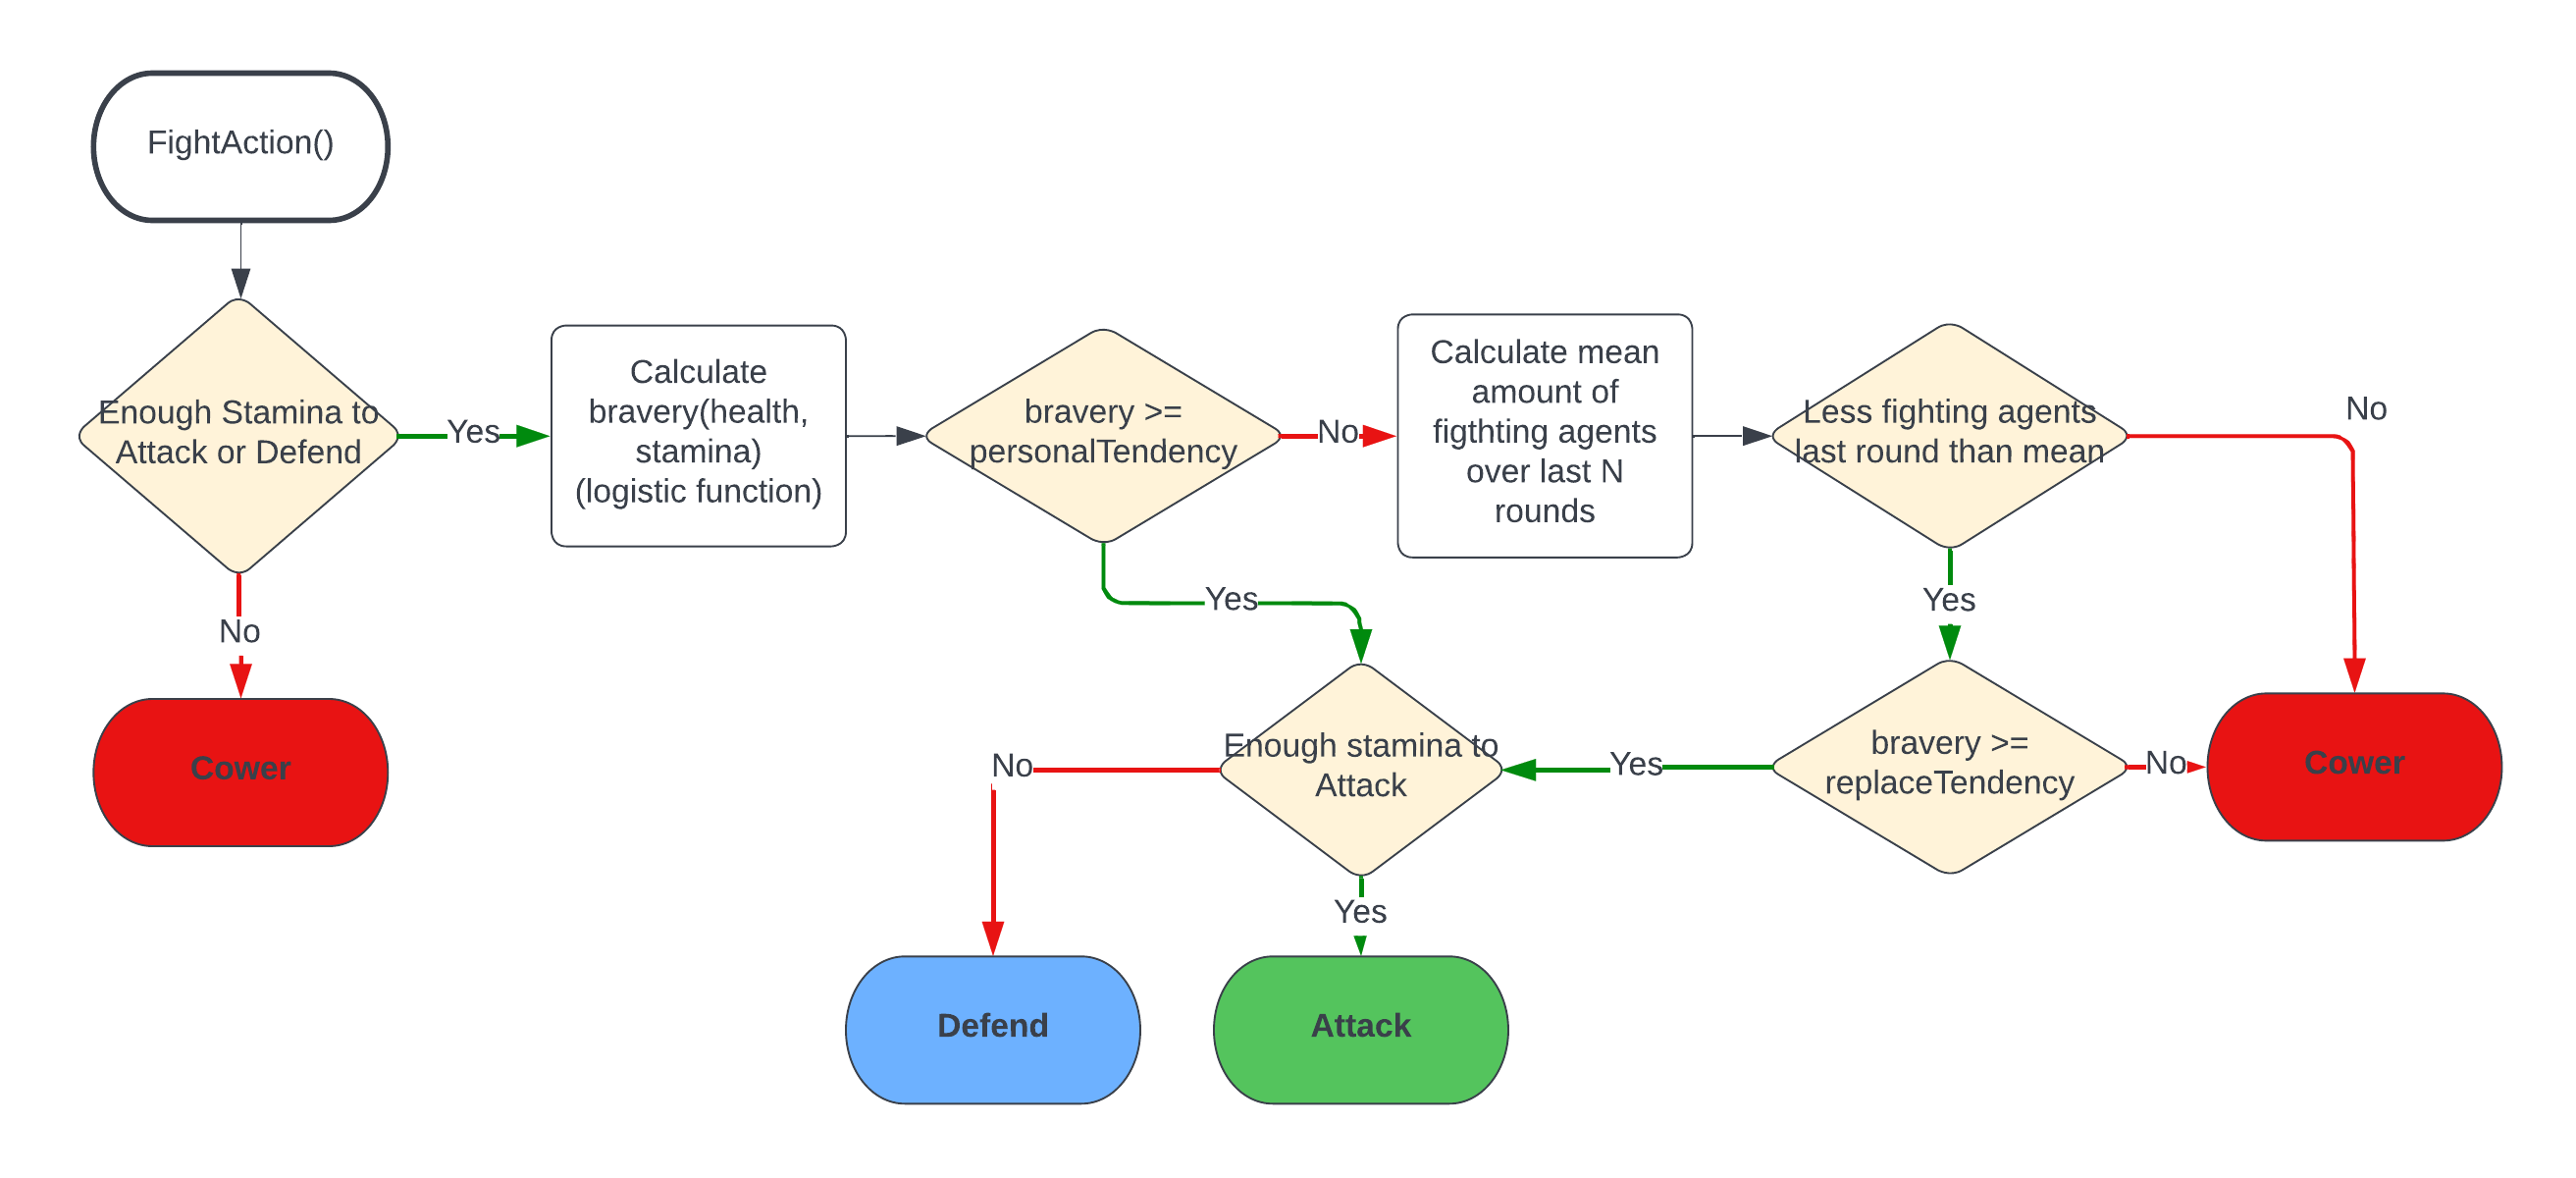
\includegraphics[width=\linewidth]{SOMAS-Agent2-Report/fightaction.png}
    \caption{Process of personal decision making}
    \label{fig:fightaction}
\end{figure}

Each agent contains two character traits, generated at the program's initialisation : \begin{itemize}
    \item \verb|personalTendency| $\in[0,1]$ : the agent's tendency to fight
    \item \verb|replaceTendency| $\in[0,1]$ : the agent's tendency to replace non-fighting agents
\end{itemize}
Additionally, each time \verb|FightAction()| is called, a fluent variable \verb|bravery| is computed such as $$\verb|bravery|(\verb|health|, \verb|stamina|) = \frac{0.5}{1+e^{-0.01(health-500)}} + \frac{0.5}{1+e^{-0.005(stamina-1000)}}$$
which is a combination of two spread logistic functions over the range of \verb|health| and \verb|stamina|.

 \verb|bravery|, $\in [0,1]$, represents the current "confidence"\footnote{The variable bravery was not named confidence in order to avoid mistaking it with the confidence in the leader.} an agent has depending on its state : the more health and stamina it has, the braver it feels.

 \paragraph{Initial decision}

 By comparing its current \verb|bravery| to its \verb|personalTendency|, the first makes a decision to act or cower. If $\verb|bravery| > \verb|personalTendency|$, it will end the function and return either Attack or Defend. If not, it will first decide to cower.


 \paragraph{Replacement decision}

 If the answer to the initial decision was Cower, the agent will then use the history mechanism (its memory) to observe the overall trend in decisions. It computes the mean of fighting/defending agents over the last $N$ rounds, and if it find that last round was lower than the mean, it will reconsider its decision.

 Then, if  $\verb|bravery| > \verb|replaceTendency|$, it will either Attack or Defend. Else, it will stay in a cowering state.

\paragraph{Not-implemented : damage estimation}

This part was not implemented because at some point, it was decided on the infrastructure side that agents would not have access to the entire set of current agents decisions, and that peer-to-peer communication would be limited.

An additional test was supposed to be made, where the agent would try to estimate the current damage and defense based on the current set of decision, and possibly decide to act if it found these values to be too low. The decision would have followed the same process as before.

\subsection{Behaviour}
Overall, with the right parameters, the agents will try to act as much as they can while preserving their own health. They will occasionally override their own decision for the greater good, to try to replace cowering agents.


\section{Manifesto}

Influenced by the concept of relevant expertise aggregation, we thought that we could treat our agent as an "expert singleton" as far as leadership candidacy is concerned. We decided that we will be quantifying our expertise in order to be able to derive what values we could reasonably set in our 'manifesto' i.e. the terms of leadership we put forward in any election. This quantification metric, which can be also thought as an equivalent indicator of credibility in a trust framework, was set as follows:(Explanation of 2 eq). 

Through \verb|ManifestoEffectiveness| we can measure how well we perform when we request a fight decision or loot imposition. It should also be highlighted that expertise does not always increase, but instead it can decrease as well (so it is different to the concept of experience). In order to derive the term length, we map our expertise to a range between 0 and 4 and add it to a default value of 1. In other words, in the very beginning, if we don't have any expertise at all, we request a term length of 1, (which is reasonable due to our lack of expertise), but as we start to gain expertise the term length will dynamically adjust in the range [1,5]. Moving on to fight decision power, we wanted to be able to take into consideration the previous leaders' manifestos and whether they were deposed, since we thought that perhaps the cohort would not trust a new leader with the same manifesto as a previous leader who was deposed. More specifically, we start by checking whether the previous leader had fight decision power and whether he was deposed. If both are true, we take our expertise and subtract from it a small negative bias. Then, if this total value is greater than a threshold, we set \verb|fightDecisionPower| to true in our manifesto. An equivalent logic has been implemented for determining whether \verb|lootDecisionPower| should be true. Finally, for deriving the no-confidence percentage required for our leader to get deposed, we map our expertise to a range of [-10\%, 10\%] and add this value to a default percentage of 51\%, considering that if we do not have any expertise, a simple majority of 51\% would be a reasonable value, but as we start having more expertise, that value should be dynamic and within the range [41\%,61\%], since a more 'expert' leader is more credible and trustworthy, therefore shouldn't be as easy to depose (and vice versa for a less expert leader).\\

\section{Fight strategy} If this agent is elected as a leader, we will have the following fighting strategy: we will propose that agents with Health lower than the bare minimum should Cower, thus forcing those who are the most vulnerable to survive and regenerate health; agents with Health greater than the baseline and attack and defend greater than the minimum required will be suggested to attack and defend as it is their moral obligation to perform these actions and lead the fight; remaining agents that do not fall within these parameters will be free to perform their own Actions. We will choose to broadcast the proposals of other agents with a similar strategy (?). Elasticity will be used to allow a range for Minimum and Baseline values to be checked with the Proposal if they are satisfied.(Explain Elasticity?)\\

\section{No-confidence vote}
To handle the no-confidence vote for the leader, at the end of each level, we implement a generic social capital framework. More specifically, we takes as 'events' information about the game yielded under that agent's leadership - such as remaining agents after each round/level, fighting statistics for the leader etc. Then, we use 'event handler' functions to convert these to useful quantitative metrics - such as how many (if any) times they were a leader before, if they were voted out in on-confidence, the rate at which the agent pool is decreasing, how frequently agents are given the floor for proposals etc.(...). These metrics are in turn normalized with respect to their global averages (otherwise their magnitudes are meaningless; normalizing gives an indication of how much better or worse the leader is performing compared to other leaders). Then, these are selectively weighted and summed to yield social capital values for the current leader. Namely, 'trustworthiness' is measured as how positively their leadership impacts the collective, through combining the survival rates under their current and previous leaderships (weighting the former more). 'Networks' are (tenuously...) measured as the rate, again from both current and previous leaderships, at which the leader broadcasts proposals our agent has submitted to them. This sort of quantifies how communicative the leader is. Finally, 'Institution' is measured as a combicnation and how successfully they wielded it

\\

\section{Election of a leader}To select a preference for the leader, we again take into consideration two of the metrics used in the social capital framework, but only the two values, but also the manifesto of the prospect leaders. More specifically, to vote for a leader we compute a score for each prospect leader, based on the following parameters. If the leader requires a fight imposition, we add a small negative bias to the score of the prospect leader. This is, because especially if the leader has not been elected before and has no expertise, we prefer that he does not impose(/ propose?) a fight. We rather want that this decision comes from all the agents collectively. Equivalently, we add a small negative bias if the leader requires a loot imposition. Additionally,another parameter that we take into account is the Sot(overthrow percentage+term length). We sum the overthrow percentage and term length for each prospect leader and then rank them in descending order (the one with the smallest overthrow percentage+term length gets the highest points). Now, if the leader has been elected before, we also consider the two social capital parameters mentioned before. Finally,we weigh these parameters, we sum them and we vote for the agent with the highest score. The highest weights are given to the parameters associated with past leadership data, because we think that expertise is crucial for a leader.\\

\section{Weapon and shield selection}Additionally, considering that our agent can only attack or defend if our stamina is greater than our BonusAttack, we decided that whenever we choose to fight, we should fight with the weapon with the highest BonusAttack given our Stamina at that point. Equivalently, our agent always chooses the Shield with the highest BonusDeafence.\\

\section{HP pool donation}In terms of HP(Health Points), our agent always donates to the common pool if his health points our greater than a threshold. The amount of health points given at the end of each level is dynamically adjusted according to: (explain math formula).


\chapter{Team 3 Agent Design}\label{team_3_agent_design}

\section{Agent Implementation}
    
    \subsection{The Ideology}

        At the heart of our agent design is a computational implementation of \textit{preference utilitarianism}. This form of contempary philosophy is characterised by the maximisation of actions that forfil the interests of those bodies involed \cite{hare1981moral}. It includes a basic assumption that these interests are, at least in part, influenced by some future projections based on the combination of ones; current state, history and social interactions. If we define the `bodies involved' as all agents within the environment, we can split them into two weighted catagories. The first (weighted high) being a Trusted Social Network (TSN) and the second (weighted low) being the remaining agents. With this network defined, we can summerise this ideology with respect to the cooperative survial game as; the choice of actions that maximise the interests of the self and the TSN whilst endevouring to satifice all other agents involved. By definition, a reduction in TSN entails an increase in self-interest. 
        
        A key part of Preference Utilitarianism is that interests are based upon future projections. In the contet of this game, these projections can be heavily influenced by collective risk analysis and social interactions, infering that a `selfish action' may not be in an agents best interst in the long term. Therefore, the idea of maximising self-interest does not always entail acting selfishly, as the abjective of the game is to win via collaberation. This phanomenon will be addressed later in this section when the ideas of utility and social captial are introduced. A perticularly interesting aspect of this direction is the assumption that every agents definition of satifaction and preference is unique, which could be consiered true in this game.  
        
        All this points towards the fact that our agent must be environmentally adaptable to the changing circumstances of the social network. This can be seen as a dynamically scaling network of agent-to-agent relationships, where; actions, collective knowledge aggregation and peer-to-peer transactions influence social capital scores and determin the strength of these relationships. Eventually, a strong enough relationship will see an agent labeled as `trusted' and being added to the TSN. But how is this all decided? 

        % add parts about our high level opinions on governance, social capital, utility, effectiveness and fairness

        \begin{figure}[htb]
            \centering
            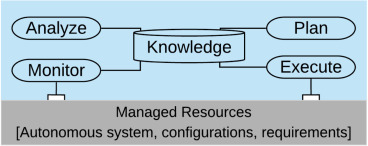
\includegraphics{006_team_3_agent_design/FIGS/mapek.jpg}
            \caption{MAPE-K framework}
            \label{fig:mapek_framework}
        \end{figure}

        The ideological architecture presented in Figure \ref{fig:mapek_framework} falls within the assumption of the self-organising MAPE-K interaction framework \cite{mapek}. In this framework, an agent monitors the environment in order to make the most balanced decision, with a strong personal bias as a general preference. By performing some form of analysis, anomalous decisions that result in un-favourable outcomes within an event horizon can be detected. With these actions discarded, a sequence of actions can be devised with the aim to improve the agents state within this event horizon. This all fits into Ostron's perspective on the benefits of non-centralised governance, which in the context of multi-agent systems, may only function in the presence of ubiquitous common knowledge \cite{pitt}. 
        


        
        
    \subsection{Autonomous Decisions \& Semi-Reinforcement}

        Our agent's decision is based on a \textit{Semi-Reinforcement Social-Construct} learning algorithm. This approach utilises a proven-to-be-effective dynamic weight-updating model applied to data collected via various social interactions as well as internal states. These interactions are all within the boundaries determined by the concept of an open society, where agents perform such social actions as submitting collective action proposals, sharing opinions and trading. In other words, the decisions of our agent will be reinforced using heuristics based upon social capital, utility and collective risk analysis. With the goal state being to escape the Pit(t). 

        
        At this point, it is crucial to stress the function of social capital when it comes to \textit{reward} and \textit{punishment}. It can be simplified to a recognition bason on a fellow agent's effect on the individual, be it beneficial or detrimental. This should not be confused with metrics such as \textit{fairness} or \textit{effectiveness}, which are used when performing collective risk analysis. However, all of these metrics are unqiuely set for each agent and are dependent on parameters extracted from interactions with said agent (or opinions shared by the community about said agent). 

        To summarise, our agent will form decisions based on it's own knowledge, weighted preference aggregates from trusted social counterparts and the level of contribution to the collective. The trade-off between short-term and long-term satisfaction will ultimately depend on the current state, histocial data (for our agent's experiences) and future projections.  
        % not sure i like this section.... it doesn't really talk aboyt what our algorithm dose and why........ it is weight updating..... so lets talk about tht

\section{Social Interaction \& Utility Interpretation}

One of the greatest challenges when working on the agent design was an algorithmic representation of social capital. We wanted to not only represent social relations as knowledge in a system, but also use this knowledge to produce suitable actions. It was decided to implement a utility function to make the computational representation as close as possible to the theoretical reasoning. It is used, and subsequently updated, by our agent to represent ever changing relationships. Therefore, the output of this function is a list mapping the id of every agent to their utility, where the \textit{utility} is based on the aggregated weighted average of the following three actions:
        
\textit{Trade interaction}: The agent introspectively punishes when the resource trade process is rejected and rewards when the resource is traded. In the case of a rejection, retributive justice is applied depending on the current relationship strength between the agents and their utility score. This ensures that the punishment never breaks strong social bonds unless circumstances deem it absolutely necessary. Using this as our base princpal, accepted transactions resulted in larger rewards, introducing possitive reinforcement and forgiveness to sustain social bonds. These rewards and punishments are manifested as increasing or degrading the resource utility score. Relationships are determined by an agents current overall utility score. The impementation can be seen in Algorithm \ref{alg:1}. 

\begin{algorithm}[htb]
    \caption{Resource Utility}\label{alg:1}
    \begin{algorithmic} 
    \scriptsize
    \Require $agent\_id, resource\_utility$
    \Ensure $resource\_utility\_output[0-15]$
    \If{Initial State}
    \State $resource\_utility \leftarrow $ Start Value
    \EndIf
    \If{Trade Rejected}
    \If{Strong Relationship}
    \State Slighty Degrade $resource\_utility$ 
    \EndIf
    \If{Basic Relationship}
    \State Degrade $resource\_utility$
    \Else
    \State Strongly Degrade $resource\_utility$
    \EndIf
    \EndIf
    \If{Trade Accepted}
    \State Strongly Incrase $resource\_utility$ 
    \EndIf
    \end{algorithmic}
    \end{algorithm}



\textit{Proposal performance}: If our agent was asked about their fight decision preference, and the resulting proposal confirmed this action, a reward is given to the agent responsible. In the opposite case, where our preference was denied after consultation, a punishment would be applied. To once again introduce possitive reinforcement, a punishment will not be applied until the condition is met multiple times. Again, these rewards and proposals are applied as increasing or decreasing the agents proposal utility, as shown in Algorithm \ref{alg:2}. Intuitively, this score could never update for a given agent, as it requires both contact to be made and their proposal to be granted access to the floor. 

\begin{algorithm}[htb]
\caption{Proposal Utility}\label{alg:2}
\begin{algorithmic} 
\scriptsize
\Require $agent\_id, proposal\_utility$
\Ensure $proposal\_utility\_output[0-15]$
\If{Initial State}
\State $proposal\_utility \leftarrow$ start value, $\; ACC \leftarrow 0$
\EndIf
\If{Consulted $\land$ Proposal Accepted $\land ~\neg$Our Decision}
\State $ACC \leftarrow ACC+1$
\If{$ACC \geq$ Threshold}
\State Degrade $proposal\_utility$, $\; ACC \leftarrow 0$
\EndIf
\EndIf
\If{Consulted $\land$ Proposal Accepted $\land$ Our Decision}
\State Increase $proposal\_utility$, $\; ACC \leftarrow 0$
\EndIf
\end{algorithmic}
\end{algorithm}


\textit{Biased chair}: This is based on the assumption that our strategy is always best. If there is a difference between the internally calculated fight action and the obliged action determined by the agreed proposal, then the chair's strategy is considered sub-optimal and a punishment is applied. To allow of any initial transients, this punishement is only applied after the chair has been in power for a number of rounds. This contraint however, does not apply to the reward given if the actions match. In this case, the chair's strategy would be considered optimal. Algorithm \ref{alg:3} shows how rewards and punishments are applied by increasing or decreasing the chair utility. 

\begin{algorithm}[htb]
\caption{Chair Utility}\label{alg:3}
\begin{algorithmic} 
\scriptsize
\Require $agent\_id, chair\_utility$
\Ensure $chair\_utility\_output[0-15]$
\If{Initial State}
\State $chair\_utility \leftarrow$ Start Value, $\; N \leftarrow 0$
\EndIf
\If{Obligated Decision $\neq$ Our Decision}
\State $Rounds\_in\_power \leftarrow Rounds\_in\_power+1$
\If{$Rounds\_in\_power \geq$ Threshold}
\State Degrade $chair\_utility$
\EndIf
\EndIf
\If{Obliged Decision $=$ Our Decision}
\State Increase $chair\_utility$
\EndIf
\end{algorithmic}
\end{algorithm}

To obtain an overall utility score, shown in Algorithm \ref{alg:4}, both chair and resource utilities are weighted equally. Due to the nature of round/level operation within the game, \textit{proposal utility} has a lower level of contribution to the weighted average. This decision was made according to the \textit{participation principle}, and the fact that the decision frequency is lower than its application. With all of the above algorithms; thresholds, rewards and punishments should be determined during testing and my could be based on a percentage change of current values. This logic applies to all thresholds embedded with the alogrithms in this team's section. If a threshold value is specificed, it is for the readers convience of readability.                    


\begin{algorithm}[htb]
\caption{Utility}\label{alg:4}
\begin{algorithmic} 
\scriptsize
\Require $agent\_id, chair\_utility, resource\_utility, proposal\_utility$
\Ensure $utility\_score[0-15]$
\If{End of Round}
\State $total\_utility \leftarrow average\{chair\_utility \times w_1, resource\_utility \times w_1, proposal\_utility \times w_2\}$
\EndIf
\end{algorithmic}
\end{algorithm}


\clearpage

\section{Borda Count for Distributive Justice }

Canons of judicial conduct, $C_0$ : \textit{Needs} and $C_1$ : \textit{Productivity}, with their effects on the commonwealth, are measured and reinforced through the process of updating respective weights. These are the most viable features for our design, both given a constant value of 5 as an initial condition for every fellow agent. As per the algorithm presented below, weights for these will be updated accordingly, thereby forming a plausible metric indispensable for suitable decision-making.

The final \textit{borda score} returned for each agent can be further used as a viable representation of \textit{fairness}. Hence, the agent framework could be sorted based on the fairness level, thereby implementing the principle of \textit{Borda Voter}.

It suffices to note that $w_1$ is updated according to the health and stamina of each agent, whereas $w_2$ is changed by a simple fact, whether an agent was active in battle\footnote{fought or defended actively} or just cowered.


\begin{algorithm}[htb]
\caption{Borda Score}\label{alg:5}
\begin{algorithmic} 
\scriptsize
\Require $agentMap, w_1, w_2, needs, productivity$
\While{}{$i$ in $agentMap$}
\State $Update Weights$
\State $Score \leftarrow w_1 \times needs + w_2 \times productivity$
\State $fairness[agentID] \leftarrow Score$
\EndWhile
\State $sort(fairness)$\\
\Return FAIRNESS
\end{algorithmic}
\end{algorithm}
%%%%%%%%%%%%%%%%%%%%%%%%%%%%%%%%%%%%%%%%%%%%%%%%%%%%%%%%%%%%%%%%%%%%%%%%%%%%%%%%%%%%%%%%

\begin{algorithm}[htb]
\caption{Update Weights [W1]}\label{alg:6}
\begin{algorithmic} 
\scriptsize
\Require $agentMap, healthINIT, staminaINIT,healthNOW, staminaNOW$
\State healthINIT $\leftarrow agentMap.healthINIT.ALL$
\State staminaINIT $\leftarrow agentMap.staminaINIT.ALL$
\If{$updateW1$}
\State healthNOW $\leftarrow$ health from thread
\State staminaNOW $\leftarrow$ stamina from thread
\State HP $\leftarrow$ healthINIT[agent.ID] $-$ healthNOW[agent.ID]
\State ST $\leftarrow$ staminaINIT[agent.ID] $-$ staminaNOW[agent.ID]
\If{$ST>0$}
\State $W1~+= 0.2$
\Else
\State $W1~-= 0.2$
\EndIf
\If{$HP>0$}
\State $W1~+= 0.2$
\Else
\If{$HP = 0$}
\State $W1 = W1$
\Else
\State $W1 -= 0.2$
\EndIf
\State $W1~-= 0.2$
\EndIf
\If{$W1>10$}
\State $W1=10$
\EndIf
\If{$W1<0$}
\State $W1 = 0$
\EndIf
\State healthINIT[agent.ID] $=$ healthNOW
\State staminaINIT[agent.ID] $=$ staminaNOW
\Return W1
\EndIf
\end{algorithmic}
\end{algorithm}
%%%%%%%%%%%%%%%%%%%%%%%%%%%%%%%%%%%%%%%%%%%%%%%%%%%%%%%%%%%%%%%%%%%%%%%%%%%%%%%%%%%%%%%%


\begin{algorithm}[ht]
\caption{Update Weights [W2]}\label{alg:7}
\begin{algorithmic} 
\scriptsize
\Require $agentMap, healthINIT, staminaINIT,healthNOW, staminaNOW$
\If{agentFoughtAndDefended}
\State $W2~+= 0.2$
\Else
\State $W2~-= 0.2$
\EndIf
\If{$W2<0$}
\State $W2 = 0$
\EndIf
\If{$W2>10$}
\State $W2 = 10$
\EndIf
\State
\Return W2
\end{algorithmic}
\end{algorithm}
%%%%%%%%%%%%%%%%%%%%%%%%%%%%%%%%%%%%%%%%%%%%%%%%%%%%%%%%%%%%%%%%%%%%%%%%%%%%%%%%%%%%%%%%

\clearpage
\section{Agent Operation Cycle}

All agent functionalities shown in the form of the game cycle graph are presented in figure \ref{fig:agent_model}. After each level commences the agent makes a decision regarding a donation to the common pool resources. Later, a sequence of decisions must be taken starting from the fight or flight, finishing on the resource trade and governance approach.

\begin{figure}[htb]
    \centering
    
\includegraphics[scale=0.35]{006_team_3_agent_design/FIGS/diagram.png}
    \caption{Agent Model Draft}
    \label{fig:agent_model}
\end{figure}

\clearpage


\section{Fight, Defend \& Cower Decision}

%MODIfIED:

Arguably, the decision about agent allocation as a fight resource is the most essential in the game. It can be perceived as an individual preference, as well as joint distribution based on social will. In this section the internal fight decision-making process will be discussed, followed by the proposal formation technique.


    \subsection{Internal fight decision}

        The first part is an internal function to see if our agent is going to fight or flee. In this part, the Health points, resource confidence\footnote{attack, shield} and the number of cowering decisions until the current state.
        To maximise self-satisfaction and avoid jeopardy, the agent will always cower if its health point is smaller  than  1.25 $\times$ average(HP) of the agents or 1.25 $\times$ stamina(HP). Otherwise, based on which resource confidence is higher, it will defend or attack as outlined below.

        On the other hand, if our agent is not in the internally-defined edge case\footnote{that is, it has not a critically low level of parameters required to survive the round}, and he has cowered for more than $\alpha$\footnote{starting with $\alpha~=~3$} rounds, it will fight. The accumulator parameter $\alpha$ will be increased continuously every 3 levels by 1; hence, the agent becomes more selfish the more levels increase. the implementation of this is shown in Algorithms \ref{alg:8}-\ref{alg:10}. 


\begin{algorithm}[htb]
\caption{Internal Fight Decision}\label{alg:8}
\begin{algorithmic} 
\scriptsize
\Require $agent\_id, HP\_total, HP, Damage, Shield$
\Ensure Possible to vote
\If{$HP < 1.05 \times average(HP\_total) \lor Stamina < 1.05 \times average(STAMINA\_total)$}
\Return COWER
\EndIf
    \If{$Shield \leq Damage$}
\Return ATTACK
\EndIf
\If{$Shield > Damage$}
\Return DEFEND
\EndIf
\end{algorithmic}
\end{algorithm}

\begin{algorithm}[htb]
\caption{Edge Case}\label{alg:9}
\begin{algorithmic} 
\scriptsize
\Require $agent\_id, HP\_total,Stamina\_total, HP, Stamina, Damage, Shield$
%\Ensure $Possible\_to\_vote$
\If{$Stamina < 0.6*average(Stamina\_total) \lor HP < 0.6*average(HP\_total)$}
\Return COWER
\EndIf
\end{algorithmic}
\end{algorithm}

\begin{algorithm}[htb]
\caption{Change Decision}\label{alg:10}
\begin{algorithmic} 
\scriptsize
\Require $agent\_id, HP\_total, HP, Damage, Shield$
\Ensure $Possible\_to\_vote$, $\alpha$ initially 0, increments every 5 rounds
\If{$\neg EdgeCase()$}
\If{$AD \leq DT \land round \geq \alpha+3$}
\Return ATTACK
\If{$AD > DT \land round \geq \alpha+3$}
\Return DEFEND
\EndIf
\EndIf
\EndIf
\end{algorithmic}
\end{algorithm}

\pagebreak

\subsection{Threshold Proposal for Fight Decision}
    
The second fight decision is required to form a viable proposal based on the internal needs and necessary actions for the collective to succeed. In all, in this design agent must operate on 6 thresholds; three for the \textit{Attack}\footnote{this concerns HP, Stamina, BonusAttack} and three for the \textit{Defence}\footnote{this concerns Stamina and BonusDefence only}. These will be used to effectively obtain the proposal map which defines each agent's desired state for the level. There are three factors that impact the value of the proposal thresholds.
    
The first one is based on the internal agent's decision and shown in Algorithm \ref{alg:thresh1}. It was decided that if our agent cowers, but is currently in a good state\footnote{which would still allow it to fight}, then the HP and Stamina threshold for people to attack or defend should be lower than the social average. However, if our agent wants to cower and he is in bad shape, the HP and Stamina threshold for the proposal could, in fact, be higher than the average. For the attack and defend threshold, we will propose approximately the average value be in place. On the other hand, if an agent decides to fight, then he will ask for an average threshold, as it is beneficial for a higher proportion of agents to fight in order to distribute the damage.
 


\begin{algorithm}[htb]
\caption{Threshold Decision (Part 1)}\label{alg:thresh1}
\begin{algorithmic} 
\scriptsize
\Require $agent\_id, HP\_total, HP, Damage, Shield$
%\Ensure $Possible\_to\_vote$
\If{$ourHP \geq average(HP\_total) \land decision = COWER$}
\State $HPthreshold1 \leftarrow 1.7 \times average(HP\_total)$
\EndIf
\If{$ourSTAMINA \geq average(STAMINA\_total) \land decision = COWER$}
\State $STAMINAthreshold1 \leftarrow 1.7 \times average(STAMINA\_total)$
\EndIf
\If{$ourHP < average(HP\_total) \land decision = COWER$}
\State $HPthreshold1 \leftarrow 0.7 \times average(HP\_total)$
\EndIf
\If{$ourSTAMINA < average(STAMINA\_total) \land decision = COWER$}
\State $STAMINAthreshold1 \leftarrow 0.7 \times average(STAMINA\_total)$
\EndIf
\end{algorithmic}
\end{algorithm}

The second threshold, shown in Algorithm \ref{alg:thresh2} is based on the agent's trusted social network decision to fight or flight. If more than half of the group of agents we have established a bond with want to fight, the threshold is less than the average. Otherwise, it remains as before. If there is no reply from anyone in the TSN, then threshold 1 will hold. Otherwise, the weighted average of threshold 2 will be chosen, bearing in mind a substantially higher weight for the first one; that is, our agent's internal decision.

    
\begin{algorithm}[htb]
\caption{Threshold Decision (Part 2)}\label{alg:thresh2}
\begin{algorithmic} 
\scriptsize
\Require $agent\_id, HP\_total, HP, Damage, Shield$
%\Ensure $Possible\_to\_vote$
\If{Decision $=$ COWER}
\State $AttackThreshold1 \leftarrow 1.1 \times average(attackPoint)$
\State $Defence \leftarrow 1.1 \times average(defencePoint)$
\EndIf
% \Else
\If{Agent Fights}
\State $HPthreshold1 \leftarrow average(HP\_toral)$
\State $STAMINAThreshold1 \leftarrow average(STAMINA\_total)$
\State $AttackThreshold1 \leftarrow 0.4 \times average(ATTACK\_total)$
\State $DefenceThreshold1 \leftarrow 0.4 \times average(DEFENCE\_total)$
\EndIf
\If{$\geq50\%$~TSN want to fight}
\State $HPthreshold2 \leftarrow 0.7 \times average(HP\_toral)$
\State $STAMINAThreshold2 \leftarrow 0.7 \times average(STAMINA\_total)$
\State $AttackThreshold2 \leftarrow 0.6 \times average(ATTACK\_total)$
\State $DefenceThreshold2 \leftarrow 0.6 \times average(DEFENCE\_total)$
\EndIf
\If{$<50\%$~TSN want to fight}
\State $HPthreshold2 \leftarrow 1.1 \times average(HP\_toral)$
\State $STAMINAThreshold2 \leftarrow 1.1 \times average(STAMINA\_total)$
\State $AttackThreshold2 \leftarrow 1.1 \times average(ATTACK\_total)$
\State $DefenceThreshold2 \leftarrow 1.1 \times average(DEFENCE\_total)$
\EndIf
\If{NO REPLY FROM TSN}
\State Only use $threshold1$
\EndIf
\If{REPLY FROM TSN}
\State $0.8\times threshold1 + 0.2 \times threshold2$
\EndIf
\If{The agent asked $\geq$ 10\% of fellow agents}
\State $1.1 \times (0.8\times threshold1 + 0.2 \times threshold2)$
\EndIf
\If{The agent asked $<$ 10\% of fellow agents}
\State $0.9 \times (0.8\times threshold1 + 0.2 \times threshold2)$
\EndIf
\end{algorithmic}
\end{algorithm}


Ultimately, the third threshold is a metric taking into consideration a group of agents from 3 different categories. These are to be understood as a social classification of individuals who, either, have the highest needs, are 'neutral' in the context of social capital, or are simply non-effective free-riders. Based on the sorted array of agents, thanks to the Borda score, it is possible to establish the threshold. Even though this might be seen as a relatively convoluted way of gathering data about social behaviour, it allows for establishing a just collective action without an undesirable elitism component.


Once again, our agent must also consider fight proposals on the floor. Algorithm \ref{alg:propagree} shows that any proposal whos conditions are within a $\pm 10\%$ range of ours will be accpeted. 

\begin{algorithm}[htb]
\caption{Proposal Agreement}\label{alg:propagree}
\begin{algorithmic}
\scriptsize    
\Require $agent\_id, HP\_total, HP, Damage, Shield$
\If{Proposal Agreement}
\If{ProposalThresholds are within $\pm 10\%$(ourThresholds)}\\
% \If{$thresholdHP < 1.1 \times thresholdHPProposal \land
% thresholdHP > 0.9 \times thresholdHPProposal$}
% \If{$thresholdStamina < 1.1 \times thresholdStaminaProposal \land
% thresholdStamina > 0.9 \times thresholdStaminaProposal$}
% \If{$thresholdAttack < 1.1 \times thresholdAttackProposal \land thresholdAttack > 0.9 \times thresholdAttackProposal$}
% \If{$thresholdDefend < 1.1 \times thresholdDefendProposal \land thresholdDefend > 0.9 \times thresholdDefendProposal$}\\
\Return ACCEPT
\Else\\
\Return REJECT
% \EndIf
% \EndIf
% \EndIf
\EndIf
\EndIf
\end{algorithmic}
\end{algorithm}






\clearpage

\section{Voting Decision}

The concept of institutionalised power and the need for self-organisation has been briefly signposted in the very first section of this agent-design document. Elinor Ostrom's set of working rules directed towards an institution for all self-governing agent commons was a principal bearing for the established voting approach. In the \textit{linear-public-goods-type} game, where the resources are scarce and profiles, just like in this design approach, preferentially individualistic, it is essential to form voting decisions whose focal point is narrowed onto several parameters; the effectiveness measure, the Trusted-Network-benefit, and the Agent-benefit. That is because, in an ideal case, each individual should be 'satisficed' with a good-enough solution to, both, survive and enhance the commonwealth. That, in the long-run should drastically increase the chances a positive outcome of the game.

The first one measures the effectiveness of the chair by directly measuring the increase in casualties in each subsequent level\footnote{this corresponds to a particular agent's 'reign' time}. Hence, if more agents died on the given level $N$ than $(N-i)$, where $i \in$ \{levels on which the chair was governing\}, then the chair of this level was less effective than the chair of the concerned beforehand.

The trusted-network-benefit parameter is true if and only if the current chair is part of the agent's TSN. This is to verify whetherer the potentially unfavourable decision of the governor should be condoned due to the already established relationship. Secondly, the agent-benefit parameter aims to measure if the current chair's actions aligh with the following:

\begin{enumerate}
    \item If for our agent $X$ and its internal decision $Y$ the resultant joint vote outcome is $Z$ then the following holds
    \begin{equation}
        \exists x, \forall y, \forall z, (y(x) \rightarrow z) \rightarrow agent\_benefit = true
    \end{equation}
    
    \item For our agent $X$ and the common resource $R$, the following holds:
    \begin{equation}
        \exists x, \forall r, ((askfor(x,r) \land granted(x,r)) \rightarrow agent\_benefit = true
    \end{equation}
    \item For our agent $X$, any other agent $X'$, Trusted Social Network $T$, common resource $R$ the following holds
    \begin{equation}
        \exists x, \forall x', \forall r, \neg granted(x,r) \land granted(x',r) \land \neg member(x',t) \rightarrow agent\_benefit = false
    \end{equation}
\end{enumerate}

In the actual voting function, the algorithm aims to use all aforementioned parameters in deciding whether the no confidence vote is necessary. This is determined through the balanced parameter values which, in certain cases, might result in \textit{forgiveness}. The decision is taken based on effectiveness first to consider the greater good, but only if our agent is already satisfied; certainly not in case of personal existential jeopardy.

In any scenario, there might be a need to vote for a new chair in case the current one gets deposed. This process is initiated based on the manifesto proposed by each nominee. Algoritm \ref{alg:confidence vote}, presented below, aims to cast a vote that maximises own benefit.

\begin{algorithm}[htb]
\caption{Confidence Vote}\label{alg:confidence vote}
\begin{algorithmic}
\Require $Chair.ID,action\_our\_agent\_did, Boolean ResourceGiven$
\State $Counter\_not\_agent\_benefit = 0$
\State $Counter\_not\_effective = 0$
\State $vote = 1$ 
\State $effective = effectivenessMeasure()$
\State $AgentBenefit = updateAgentBenefit(action_done, ResourceGiven)$
\State $TrustedNetwork = updateTrustedNetwork(chairID)$
\If{$\neg Effective$}
\State Counter\_not\_effective = Counter\_not\_effective + 1
\Else  
\State Counter\_not\_effective = 0
\EndIf
\If{$\neg AgentBenefit$}
\State Counter\_not\_agent\_benefit = Counter\_not\_agent\_benefit + 1
\Else
\State Counter\_not\_agent\_benefit = 0
\EndIf
\If{$TrustedNetowrk \land Counter\_not\_effective > 2$}\\
\Return Vote = 0
\EndIf
\If{$TrustedNetwork \land Counter\_not\_agent\_benefit $}\\
\Return Vote = 0
\EndIf
\If{$Counter\_not\_effective > 1$}\\
\Return Vote = 0
\EndIf
\If{$Counter\_not\_agent\_benefit > 1$}\\
\Return Vote = 0
\EndIf
\end{algorithmic}
\end{algorithm}

%%%%%%%%%%%%%%%%%%%%%%%%%%%%%%%%%%%%%%%%%%%%%%%%%%%%%%%%%%%%%%%%%%%%%%%%%%%%%%%%%%%%%%%%
% ALGO 14

% \begin{algorithm}
% \caption{Effectiveness Measure}\label{alg:14}
% \begin{algorithmic}
% \scriptsize
% \Require $agent\_id, HP\_total, HP, Damage, Shield$
% \State $effective \leftarrow true$
% \State $MonsterAttackINIT \leftarrow 1$
% \State $prevLevel = 0$ (initially...)
% \If{Effectiveness Measure}
% \State $MonsAtt \leftarrow getMonsterAttack()$
% \State $NumAgentsAlive \leftarrow getAgentsAlive()$
% \State $\Delta Percentage \leftarrow 1-(MonsterAttack-MonsterAttackINIT)~/~MonsterAttackINIT$
% \If{$NumAgentsAlive > prevLevel \times \Delta Percentage$}
% \State $effective \leftarrow true$
% \Else
% \State $effective \leftarrow false$
% \EndIf
% \State $prevLevel = thisLevel$\\
% \Return effective
% \EndIf
% \end{algorithmic}
% \end{algorithm}
%%%%%%%%%%%%%%%%%%%%%%%%%%%%%%%%%%%%%%%%%%%%%%%%%%%%%%%%%%%%%%%%%%%%%%%%%%%%%%%%%%%%%%%%

%%%%%%%%%%%%%%%%%%%%%%%%%%%%%%%%%%%%%%%%%%%%%%%%%%%%%%%%%%%%%%%%%%%%%%%%%%%%%%%%%%%%%%%%
% ALGO 15

% \begin{algorithm}
% \caption{Update Agent Benefit}\label{alg:15}
% \begin{algorithmic}
% \scriptsize
% \Require $agent\_id, HP\_total, HP, Damage, Shield$
% \State $TSNbenefit \leftarrow false$ (initially...)
% \State $AGENTbenefit \leftarrow true$ (initially...)
% \State $ActionDone \leftarrow$ [action from thread]
% \State $IDgiven \leftarrow$ [ID from the thread]
% \end{algorithmic}
% \end{algorithm}
%%%%%%%%%%%%%%%%%%%%%%%%%%%%%%%%%%%%%%%%%%%%%%%%%%%%%%%%%%%%%%%%%%%%%%%%%%%%%%%%%%%%%%%%

%%%%%%%%%%%%%%%%%%%%%%%%%%%%%%%%%%%%%%%%%%%%%%%%%%%%%%%%%%%%%%%%%%%%%%%%%%%%%%%%%%%%%%%%
% ALGO 16

% \begin{algorithm}
% \caption{Update Trusted Social Network (TSN)}\label{alg:16}
% \begin{algorithmic}
% \scriptsize
% \State Trusted\_network\_benefit $ \leftarrow $ false (initially...)
% \State Agent\_benefit $ \leftarrow $ true (initially...)
% \State action\_done $ \leftarrow $ [action from thread]
% \If{chairID utility $\geq$ 10}
% \State TrustedNetwrok $ \leftarrow $ true
% \EndIf
% \State
% \Return TrustedNetwork
% \end{algorithmic}
% \end{algorithm}
%%%%%%%%%%%%%%%%%%%%%%%%%%%%%%%%%%%%%%%%%%%%%%%%%%%%%%%%%%%%%%%%%%%%%%%%%%%%%%%%%%%%%%%%

%%%%%%%%%%%%%%%%%%%%%%%%%%%%%%%%%%%%%%%%%%%%%%%%%%%%%%%%%%%%%%%%%%%%%%%%%%%%%%%%%%%%%%%%
% ALGO 17
% }

% \begin{algorithm}
% \caption{Update Agent Benefit}\label{alg:17}
% \begin{algorithmic}
% \scriptsize
% \State Agent\_benefit $\leftarrow$ true (initially...)
% \If{$action_done != fightDec()$}
% \State Agent\_benefit = false
% \EndIf
% \If{CPR\_given = false $\land$ eligible("Resource")}
% \State Agent\_benefit = false
% \EndIf
% \end{algorithmic}
% \end{algorithm}
%%%%%%%%%%%%%%%%%%%%%%%%%%%%%%%%%%%%%%%%%%%%%%%%%%%%%%%%%%%%%%%%%%%%%%%%%%%%%%%%%%%%%%%%

%%%%%%%%%%%%%%%%%%%%%%%%%%%%%%%%%%%%%%%%%%%%%%%%%%%%%%%%%%%%%%%%%%%%%%%%%%%%%%%%%%%%%%%%
% ALGO 18

% \begin{algorithm}
% \caption{Eligible to take resource}\label{alg:18}
% \begin{algorithmic}
% \scriptsize
% \Require $resource,Thresholds$
% \If{resource $==$ HPPotion}
% \If{$ourHP < threshold(HPPotion)$}
% \State
% \Return true
% \Else
% \State
% \Return false
% \EndIf
% \EndIf
% \If{resource $==$ StaminaPotion}
% \If{$ourStamina < threshold(StaminaPotion)$}
% \State
% \Return true
% \Else
% \State
% \Return false
% \EndIf
% \EndIf
% \If{resource $==$ sword}
% \If{$ourAttackPoint < threshold(AttackPoint)$}
% \State
% \Return true
% \Else
% \State
% \Return false
% \EndIf
% \EndIf
% \If{resource $==$ shield}
% \If{$ourDefencePoint < threshold(DefencePoint)$}
% \State
% \Return true
% \Else
% \State
% \Return false
% \EndIf
% \EndIf
% \end{algorithmic}
% \end{algorithm}
%%%%%%%%%%%%%%%%%%%%%%%%%%%%%%%%%%%%%%%%%%%%%%%%%%%%%%%%%%%%%%%%%%%%%%%%%%%%%%%%%%%%%%%%

%%%%%%%%%%%%%%%%%%%%%%%%%%%%%%%%%%%%%%%%%%%%%%%%%%%%%%%%%%%%%%%%%%%%%%%%%%%%%%%%%%%%%%%%
% ALGO 19

% \begin{algorithm}
% \caption{Vote Next Chair}\label{alg:19}
% \begin{algorithmic}
% \scriptsize
% \Require $agent\_id, HP\_total, HP, Damage, Shield$

% \end{algorithmic}
% \end{algorithm}
%%%%%%%%%%%%%%%%%%%%%%%%%%%%%%%%%%%%%%%%%%%%%%%%%%%%%%%%%%%%%%%%%%%%%%%%%%%%%%%%%%%%%%%%

\clearpage

\section{Chair Operation}

This section outlines all responsibilities and prerogatives of the agent who is, either, nominating himself, or already being the social chair. It is crucial to assume that the chair possesses the capacity to perceive the social construction and political meta-games so that it provides an effective, efficient, and mutually satisfiable way to solve collective problems\footnote {As a wise man once said...}.

\begin{algorithm}[htb]
\begin{algorithmic}
\caption{Chair Function}\label{alg:chairfunction}
\State temp $\leftarrow$ mapAgentWhoNeedResource[0]
\If{$\neg Power\_Flag$}
\State YieldFloor() and Update fighting map according to voted proposal
\Else
\If{$Power\_Flag$}
\If{$\neg Expert\_judgement\_fight$}
\State YieldFloor() and Update fighting map according to voted proposal
\Else
\State YieldFloor() and Update fighting map according to internal threshholds
\EndIf
\EndIf
\EndIf
\If{$\neg loot\_Flag$}
\State YieldFloor() and Update resource map according to voted proposal
\Else
\If{$loot\_Flag$}
\If{$\neg Expert\_judgement\_loot$}
\State YieldFloor() and Update resource map according to voted proposal
\Else
\State YieldFloor() and Update resource map according to internal threshholds
\EndIf
\EndIf
\EndIf
\end{algorithmic}
\end{algorithm}

Algorithm \ref{alg:chairfunction} (above) combined with Algorithm \ref{alg:ballotnom} (below), outlines the way in which the ballot nomination is executed. It indicates the logic behind processing votes from each subsequent; dispute resolution, governance election or floor yielding. There is a certain number of actions the chair may execute. For the \textit{majority 'mode'} the proposal with the highest number of votes will be implemented. 

\begin{algorithm}[htb]
\caption{Ballot Nomination}\label{alg:ballotnom}
\begin{algorithmic}
\scriptsize
\State P = True
\State Loot = True
\State T = 4   (Number of rounds with no power to append TSN)
\State Threshold = 0.4
\State VodedIn = false
\State Lnv=0
\State
\If{VotedIn}
\State $P \leftarrow true$
\State $Loot \leftarrow true$
\State $Threshold += 0.1$
\State $T \leftarrow += 0.1$
\Else
\If{$\neg$VotedIn $\land$ Lnv $\geq$ 4}
\State $P \leftarrow false$
\State $Threshold -= 0.1$
\State $T \leftarrow -= 1$
\EndIf
\If{Lnv = 5}
\State $Loot \leftarrow false$
\EndIf
\EndIf
\end{algorithmic}
\end{algorithm}

On the other hand, the agent might nominate itself with the $P$ flag value being true. As a result, a dicta... ekhm... 'Expert Judgement' call can be made,  in which case the proposal having the highest level of support in the society can still be overruled. A similar approach was applied to the capability of dealing with resource allocation. The discrete value of the \textit{loot} flag determines the chair's competence; it can either be a mediator\footnote{in which case there is no direct imposition onto who is granted the resource} or execute the litigation; have a role of the judge. The set of first-order predicate logic clauses below formalises the chair operation.

For the fight proposal, the following holds

\begin{equation}
    \exists x. agent(x) \land isChair(x) \land \neg P \rightarrow Majority()
\end{equation}
\begin{equation}
    \exists x. agent(x) \land isChair(x) \land \neg ExpJudgementFight() \land P \rightarrow Majority()
\end{equation}
\begin{equation}
    \exists x. agent(x) \land isChair(x) \land ExpJudgementFight() \land P \rightarrow ExpAssignemnt()
\end{equation}

For resource allocation, the following holds

\begin{equation}
    \exists x. agent(x) \land isChair(x) \land \neg L \land \neg ExpJudgementLoot()\rightarrow Majority()
\end{equation}
\begin{equation}
    \exists x. agent(x) \land isChair(x) \land L \land ExpJudgementLoot() \rightarrow ExpAssignemnt()
\end{equation}

Now that the agent is able to execute its rudimentary tasks concerning fight decision and resource allocation, it is crucial to enrich that functionality with an internal disobedience recognition. This mechanism represents the contempt implementation by broadcasting information about the disobedience to all individuals. Each one can then take the necessary action as deemed appropriate; which in the case of the agent would be a trade embargo imposed by decreasing each disobeying agent's utility (punishment depends on each agent's Borda score), causing the agent to not trade with them eventually.
%%%%%%%%%%%%%%%%%%%%%%%%%%%%%%%%%%%%%%%%%%%%%%%%%%%%%%%%%%%%%%%%%%%%%%%%%%%%%%%%%%%%%%%%
% ALGO 20 

% \begin{algorithm}
% \caption{Disobedience Map}\label{alg:20}
% \begin{algorithmic}
% \scriptsize
% \While{i in disobey[]}
% \If{disobey[i]}
% \If{agent.ID in borda[$0:25\% len(borda)$] $\land \neg granted(r)$}
% \State agent utility $\leftarrow$ utility
% \EndIf
% \Else
% \If{agent.ID in borda[$25\%:50\% len(borda)$] $\land \neg granted(r)$}
% \State utility $\leftarrow$ utility - 1
% \EndIf
% % \Else
% \If{agent.ID in borda[$50\%: len(borda)$] $\land \neg granted(r)$}
% \State utility $\leftarrow$ utility - 2
% \EndIf
% % \Else
% \If{$granted(r)$}
% \State utility $\leftarrow$ utility - 4
% \EndIf
% \EndIf
% \EndWhile
% \end{algorithmic}
% \end{algorithm}
%%%%%%%%%%%%%%%%%%%%%%%%%%%%%%%%%%%%%%%%%%%%%%%%%%%%%%%%%%%%%%%%%%%%%%%%%%%%%%%%%%%%%%%%

%%%%%%%%%%%%%%%%%%%%%%%%%%%%%%%%%%%%%%%%%%%%%%%%%%%%%%%%%%%%%%%%%%%%%%%%%%%%%%%%%%%%%%%%
% AGLO 21

% \begin{algorithm}
% \begin{algorithmic}
% \scriptsize
% \caption{Expert Judgement : Resource}\label{alg:21}
% \If{DisobAfter - Initialdisobidience $\geq$ 0.1 $\times$ Initialdisobidience}
% \State
% \Return true
% \Else
% \State
% \Return false
% \EndIf
% \end{algorithmic}
% \end{algorithm}
%%%%%%%%%%%%%%%%%%%%%%%%%%%%%%%%%%%%%%%%%%%%%%%%%%%%%%%%%%%%%%%%%%%%%%%%%%%%%%%%%%%%%%%%

%%%%%%%%%%%%%%%%%%%%%%%%%%%%%%%%%%%%%%%%%%%%%%%%%%%%%%%%%%%%%%%%%%%%%%%%%%%%%%%%%%%%%%%%
% ALGO 22

% \begin{algorithm}
% \begin{algorithmic}
% \scriptsize    
% \caption{Expert Judgement : Fight}\label{alg:22}
% \If{InitialAgentsAlive - AgentsAliveAfter $\geq$ 0.1 $\times$ InitialAgentsAlive}
% \State
% \Return true
% \Else
% \State
% \Return false
% \EndIf
% \end{algorithmic}
% \end{algorithm}
%%%%%%%%%%%%%%%%%%%%%%%%%%%%%%%%%%%%%%%%%%%%%%%%%%%%%%%%%%%%%%%%%%%%%%%%%%%%%%%%%%%%%%%%

%%%%%%%%%%%%%%%%%%%%%%%%%%%%%%%%%%%%%%%%%%%%%%%%%%%%%%%%%%%%%%%%%%%%%%%%%%%%%%%%%%%%%%%%
% ALGO 23

% \begin{algorithm}
% \begin{algorithmic}
% \scriptsize
% \caption{Dispute Resolution}\label{alg:23}
% \State temp $\leftarrow$ mapAgentWhoNeedResource[0]
% \While{i in range(0 , len(mapAgent)-1}
% \State temp $\leftarrow$ allocate\_resources(temp, mapAgent[i+1])
% \EndWhile
% \end{algorithmic}
% \end{algorithm}
%%%%%%%%%%%%%%%%%%%%%%%%%%%%%%%%%%%%%%%%%%%%%%%%%%%%%%%%%%%%%%%%%%%%%%%%%%%%%%%%%%%%%%%%

%%%%%%%%%%%%%%%%%%%%%%%%%%%%%%%%%%%%%%%%%%%%%%%%%%%%%%%%%%%%%%%%%%%%%%%%%%%%%%%%%%%%%%%%
% ALGO 25

% \begin{algorithm}
% \caption{UpdateLnv}\label{alg:25}
% \begin{algorithmic}
% \scriptsize
% \If{$\neg VotedIn$}
% \State $Lnv += 1$
% \Else
% \State $Lnv = 0$
% \EndIf
% \end{algorithmic}
% \end{algorithm}
%%%%%%%%%%%%%%%%%%%%%%%%%%%%%%%%%%%%%%%%%%%%%%%%%%%%%%%%%%%%%%%%%%%%%%%%%%%%%%%%%%%%%%%%

%%%%%%%%%%%%%%%%%%%%%%%%%%%%%%%%%%%%%%%%%%%%%%%%%%%%%%%%%%%%%%%%%%%%%%%%%%%%%%%%%%%%%%%%
% ALGO 26

% \begin{algorithm}
% \caption{Yield Floor}\label{alg:26}
% \begin{algorithmic}
% \scriptsize
% \State floor $\leftarrow$ floor[0]
% \While{Agent in range(0, len(AgentFloor))}
% \If{$Utility[ID[I]] > utility[floor]$}
% \State floor $\leftarrow$ ID[i]
% \Else
% \State floor $\leftarrow$ floor
% \EndIf
% \EndWhile
% \end{algorithmic}
% \end{algorithm}
%%%%%%%%%%%%%%%%%%%%%%%%%%%%%%%%%%%%%%%%%%%%%%%%%%%%%%%%%%%%%%%%%%%%%%%%%%%%%%%%%%%%%%%%


\section{CPR Allocation \& Trading}

Ostrom's framework recognises that individuals are purposeful actors responding to incentives, in the context of the demand for the CPR\footnote{Common Pool Resources}. In the context of non-rivalrous, but scarce resources, she successfully argues the point that, despite a strong urge for fulfilling personal interest, the society evolves and forms effective rules which avoid the tragedy of the commons without external regulation.

The agent design approaches the process of trading resources through the perspective of \textit{fairness}. The trade is fair, as by exchanging something as by exchanging a resource the marginal utility of our agent increases, and so does for the agent agreeing to the trade. Functions presented below are formed by implementing a simple comparison mechanism between 'us' and other fellow agents. The resources concerned are \textit{swords}, \textit{shields} and \textit{potions}.

\begin{algorithm}[htb]
\caption{Agent Needs}\label{alg:agentneeds}
\begin{algorithmic} 
\scriptsize
\Require $HP\_total, HP, Stamina, Stamina\_total$
\Require $InventoryAttack,InventoryDefend $
%\Ensure $Possible\_to\_vote$
\If{$ourHP < average(HP\_total)$}
\State Potion HP
\EndIf
\If{$ourStamina < average(Stamina\_total)$}
\State Potion Stamina
\EndIf
\If{$InventoryAttack > InventoryDefend $}
\State $value = (InventoryAttack - InventoryDefend)*0.9 \land$ return shield, value
\Else
\State $value = (InventoryDefend - InventoryAttack)*0.9 \land$ return sword, value
\EndIf
\end{algorithmic}
\end{algorithm}

The Algorithm \ref{alg:agentneeds} can be utilised to better understand the market situation, current demand/supply relationship and individual utilities through the perspective of personal needs. This utilisation can be seen in Algorithm \ref{alg:whototrade} and Algorithm \ref{alg:whattotrade}.

\begin{algorithm}[htb]
\caption{Who To Trade}\label{alg:whototrade}
\begin{algorithmic} 
\scriptsize
\Require $AgentNeeds, AgentNeedsValue, ResourceToTradeBroadcast$
\Require $SentMessage $
%\Ensure $Possible\_to\_vote$
\If{$ AgentNeeds == what\_other\_agent\_broadcasted \land  AgentNeedsValue>= Value\_what\_other\_agent\_broadcasted$}
\State AskToTrade with agent
\EndIf
\If{$\neg SentMessage$}
\State Check the broadcast list again
\If{$AgentNeeds == what\_other\_agent\_broadcasted$}
\State AskToTrade with agent
\EndIf
\EndIf
\end{algorithmic}
\end{algorithm}

\begin{algorithm}[htb]
\caption{What To Trade}\label{alg:whattotrade}
\begin{algorithmic} 
\scriptsize
\Require $InventoryAttack, InventoryDefence, Boolean Inventory(x)$
\Require $AgentHP, totalHP, AgentSt, TotalSt, NoTradeCounter,alpha, beta$
\Ensure $Initially\_\alpha = 0 \land \beta = 0$
\If{$ AgentHP> avg(TotalHP)*(1.15-\alpha) \land Inventory(potionHP)$}
\State 
\Return potionHP
\EndIf
\If{$AgentSt> avg(TotalSt)*(1.15-\alpha) \land Inventory(PotionSt)$}
\State 
\Return potionST
\EndIf
\If{$NoTradeCounter>4$}
\State $\alpha \leftarrow \alpha$ +0.5
\State $\beta \leftarrow \beta$ +1
\EndIf
\If{$InventoryAttack>InventoryDefence$}
\State 
\Return (median+beta) best sword 
\EndIf
\If{$InventoryAttack<=InventoryDefence$}
\State 
\Return (median+beta) best shield 
\EndIf
\end{algorithmic}
\end{algorithm}


The loot allocation, shown in Algorithm \ref{alg:lootallocation} solves the problem of which resources to ask from the common pool. On the first instance, it will compare its own HP and Stamina level to the average value and ask for potions if deemed necessary. For the shields and swords, which are crucial tools for survival and necessary to remain useful to the commonwealth, our agent is going to compare the average total attack points across all agents in relation to his own ones. Based on this comparison, it will ask for, either, the best, mediocre or the worst quality sword. It might, eventually, ask for no swords if decided that it is not beneficial in line with the law of marginal returns\footnote{in which case an additional weapon will not contribute to the individual utility}.

\begin{algorithm}[htb]
\caption{Loot Allocation}\label{alg:lootallocation}
\begin{algorithmic} 
\scriptsize
\Require $HP\_total, HP, Stamina, Stamina\_total$
\Require $TotalAttackpoint, TotalDefencepoint, Swords, Shields$
%\Ensure $Possible\_to\_vote$
\If{$ourHP < average(HP\_total)$}
\State  Ask for potion HP
\EndIf
\If{$ourStamina < average(Stamina\_total)$}
\State Ask for potion Stamina
\Else
\If{$average(TotalAttackpoint)>(4/len(AgentAlive))*AttackPoint$}
\State Ask for $(4/len(AgentAlive))*NumberSwords$
\Else
\State Don't ask for Attack Point
\EndIf
\If{$average(TotalDefencepoint)>(4/len(AgentAlive))*DefencePoint$}
\State Ask for $(4/len(AgentAlive))*NumberShield$
\Else
\State Don't ask for Defence Point
\EndIf
\EndIf
\end{algorithmic}
\end{algorithm}

The same reasoning is applied to all kinds of resources. Due to scarcity, it is not always the best weapon that the agent is asking for. One recognises that it might be socially penalised if having too extensive inventory compared to the others. The basis for our agent's resource allocation strategy is outlined in Algorithm \ref{alg:threshloot}. It operates on previously obtained \textit{fairness} parameter. However, our agent's proposals cannot always be guarenteeded the floor. Therefore, Algorithm \ref{alg:proplootallocation} outlines our agent's strategy for anlaysing proposals on the floor.  

\begin{algorithm}[htb]
\caption{Threshold Loot Allocation}\label{alg:threshloot}
\begin{algorithmic} 
\scriptsize
\Require $HP\_total, Stamina\_total, TotalAttackPoint,TotalDefencePoint$
ThresholdHPpotion =  average(TotHP)\\
ThresholdStaminapotion =  average(TotStamina)\\
ThresholdSword = average(TotAtackPoint)/(4/len(AgentAlive))\\
ThresholdShield = average(TotDefendPoint)/(4/len(AgentAlive))\\
\end{algorithmic}
\end{algorithm}

\begin{algorithm}[htb]
\caption{Proposal Agreement Loot Allocation}\label{alg:proplootallocation}
\begin{algorithmic}
\scriptsize
\Require $agent\_id, HP\_total, HP, Damage, Shield$
\If{Proposal Agreement}
\If{$thresholdHP < 1.1 \times thresholdHPProposal \land thresholdHP > 0.9 \times thresholdHPProposal$}
\If{$thresholdStamina < 1.1 \times thresholdStaminaProposal \land
thresholdStamina > 0.9 \times thresholdStaminaProposal$}
\If{$thresholdAttack < 1.1 \times thresholdAttackProposal \land thresholdAttack > 0.9 \times thresholdAttackProposal$}
\If{$thresholdDefend < 1.1 \times thresholdDefendProposal \land thresholdDefend > 0.9 \times thresholdDefendProposal$}
\Return ACCEPT
\Else\\
\Return REJECT
\EndIf
\EndIf
\EndIf
\EndIf
\EndIf
\end{algorithmic}
\end{algorithm}




\section{Experimental Design}

% Theory vs Practise
One of the foundational elements of a Self-Organising Multi-Agent System are the interactions between the agents as well as the limitations that an environment might impose. When designing our agents strategy on paper there were some aspects that had do be fine-tuned in an experimental approach such as the scalability of our strategy as the game progressed as well as some threshold definitions.

% Infinite Fight Loop All defend mode: Modified Fight Decision Strategy to fight more.
A particular example that we noticed during the experiments within a homogenous environment consisting of our Teams agents was the herd effect: Although our agents efficiently aligned after a certain amount of rounds, given our Utilitarianism Preference nature, the agents ended up defending alltogether that eventually ended with them being slaughtered by the perilous beast. In order to overcome this local minima that we've found and improve our agents performance, we tweaked our internal Fight Decision thresholds as well as modifying our strategy to be more aggresive at the beginning of the game, as seen in Algorithm \ref{alg:8}.

% Modifications to thresholds through experiments with our Agents and the Random Agent \ref{fig:algo8}.

% Exper
In order to provide some fair resutls, for all the experiments we've considered the total number of agents playing the game to be the same (100) as well as all the other game attributes (60 levels).
\begin{itemize}
    \item Environment with only our Agents (100), Mean Level: 22.3 (after 20 runs)
    \item Environment with Team 3 Agents (50) and Random Agents (50), Mean Level: 28.8 (after 20 runs)
\end{itemize}

% Our agents outlasted the Random Agent but still lost.
From the experiments we've run on the heterogenous environment consisting of our Teams' agent as well as the Random Agent we can conclude that although the mean level that we reached improved when interacting with others and we've managed to outlast the Random Agent, we still ended up losing the game.

\section{Evaluation \& Future Work}

Due to the nature of the assignment and extremely narrow time constraints, the team had to come up with a suitable course of action regarding the planning, executing and testing of the agent design. For any future attempts, the team believes that it would be more efficient to, not only meticulously plan and construct the pseudo-code for each subsequent agent task, but also actively gauge the example architecture to obtain threshold values in an empirical manner through the interaction with a heterogenous environment. This continuous interaction and real-life response from the simulation would certainly increase the team's productivity, and perhaps result in a more advanced algorithmic equivalence of the semi-reinforcement social construct.

In addition, by having our inventory private, other agents wouldn't be able to know what we possess. This could be one way to deceive other agents, which is by wearing a particular armour with different attributes depending on our agent's decision to fight or cower. 
\chapter{Team 4 Agent Design}\label{team_4_agent_design}

\section{Strategy Overview}

\par The overall agent strategy was formulated as surviving and escaping the pit(t) with high social contribution. The agent will come up with an action that try to strike a balance between contributing to the common good and being selfish in order to survive. When we contribute to the common good, we increase our rating of social contribution (C) , and we decrease the social contribution if we are being selfish. At the same time, we perform analysis on the social contribution of other agents as well by considering what they actually did in every round. In the following sections, we are going to describe our strategies for different aspects, including the combat round, post-combat round and governance.

\par In order to implement our strategy, we constantly calculate our own social contribution (C), other agents social contributions and the number of times agents disobeyed social contracts (fighting and looting decisions).

\par Our agent's ideology can be thought of as an Athenian in an economy of esteem. Each of our agents has the desire to survive; however, they also understand that contributing to the collective can ultimately be beneficial for themselves as well, and as such,
they also seek to interact with more esteemed members of the collective. 

\section{Combat}

\par In the combat round, our agent will consider two philosophical choices. The first one is to simply do what is best for our survival based on certain heuristics, and the second one is to perform an action that is beneficial for the common good, which is proposed in our fight manifesto.

\par For the fight decision for the combat round, our agent will "remember" past actions from other agents and assume they will choose their most common decision e.g. if an agent has cowered 70\% of the rounds so far, then we assume this agent will also cower this round. With this assumption, we can estimate the potential damage our agent will receive. If our HP is greater than the maximum damage that we may receive, this means that we will not die if we choose to fight or defend in this round. Based on this idea, we further analyse our TotalAttack and TotalDefend. If TotalAttack is greater than or equal to TotalDefend * 0.8, we will choose to attack. Otherwise, we will choose to defend. The reason why we multiply TotalDefend by 0.8 is that we think it is better to attack rather than defend in the long term hence we are able to defeat the monster as soon as possible. Last but not least, if our HP is smaller than or equal to the maximum damage that we may receive, then we should cower and try to survive. Figure 7.1 illustrates the general flow of the fight decision.

\begin{figure}
    \centering
    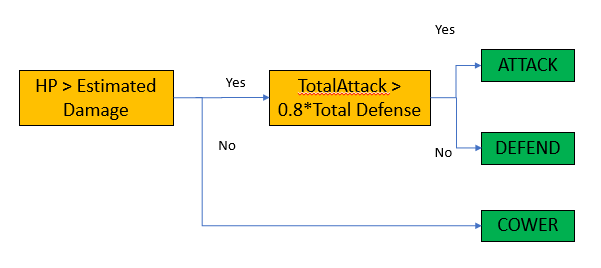
\includegraphics[width=0.5\textwidth]{007_team_4_agent_design/figures/1_fight1.png}
    \caption{Fight decision diagram.}
    \label{fig:proj_struct}
\end{figure}


\par For the fight manifesto, the threshold of ST and HP being proposed are based on the ratio of agents in each of the quantised categories of ST/HP (low, mid and high ST/HP) - see Equations 7.1 and 7.2. We also calculate a threshold for Attack and Defend points as well, which is simply the average TotalAttack and TotalDefend of all agents.
If the agent's HP or ST are smaller than threshold of HP or ST, this means that it is unwise to fight and so it makes the agent cower. Otherwise, if both HP and ST are above the threshold, the agent must fight. In this case, the agent will attack or defend if its TotalAttack and TotalDefend are greater than the Attack and Defend thresholds, respectively. If the agent is capable of both attacking and defending, this is solved by the server, following the agent's fight decision.

\begin{equation}  
thresholdHP = N_{LowHP}*(250) + N_{MidHP}*(500) + N_{HighHP}*(750)
\label{eq:equation}
\end{equation}

\begin{equation}  
thresholdST = N_{LowST}*(500) + N_{MidST}*(1000) + N_{HighST}*(1500)
\label{eq:equation}
\end{equation}

\par Our agent now may face impasse if our fight decision stand against what we are proposing in the fight manifesto e.g. our manifesto imposes our agent to fight and the fight decision is to cower. Hence, our agent must choose between the social good and a selfish behavior, which is done by altering our proposal for the fight manifesto in order to fit the fight decision (put agent's stats as thresholds). This behaviour is modeled by a random variable with high probability of not being selfish, in order to align with our agent's ideology (economy of esteem). If our agent decide to follow down the selfish path, its social contribution C is decremented. Otherwise, C is incremented. This impasse is represented in Figure 7.2.

\begin{figure}
    \centering
    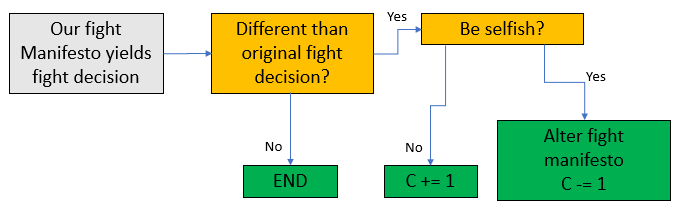
\includegraphics[width=0.5\textwidth]{007_team_4_agent_design/figures/2_fight2.png}
    \caption{Fight decision impasse diagram.}
    \label{fig:proj_struct}
\end{figure}

\par Next, we also perform voting on the fight manifesto broadcasted by the chair. Logically, our agent wants a manifesto that is similar to its proposal. 
Hence, a tolerance interval is defined for every attribute in the manifesto and if all the HP, ST, TotalAttack and TotalDefend values proposed fall within a certain range (the certain range is calculated based on our proposed values in our manifesto and the tolerance),  we vote “YES”, as this indicates a high similarity with our proposed manifesto. Otherwise, we vote “No”. 

\par After establishing a social contract on fighting decisions, we may decide to obey it or disobey it. The latter is only chosen if our agent's HP or ST are in a critical level and we are told to fight. If the two actions decided from our own heuristic and voted manifesto are not the same and we choose to obey the social contract, our C is incremented since we did something for greater common good. On the other hand, if we disobey, our C is decremented.
 

\par With these two ideas, our agent try to maximize social contribution and survive at the same time.

\par As mentioned in section 7.1, we also monitor agent's social contribution. When an agent attacks or defends with low HP or ST, it is prioritizing the common good and because of that its social contribution value is incremented. On the other hand, when an agent cowers with both high HP and ST it is prioritizing its own interests and hence, its social contribution value is incremented. This information will be used for trading and voting for a chair.

\section{Post-combat}

\par There are several actions we can perform during the post-combat round, which are donating HP to the health pool, trading with other agents and distributing loots.

\subsection{Donating HP to the Health Pool}

\par By donating HP to the health pool, we may be able to skip the combat round hence all other agents do not need to fight and take damage. This is beneficial to everyone. Therefore, if our HP is greater than a certain percentage of our total HP and our social contribution C is below a certain threshold (this means we are not contributing enough to the common good), we will donate a fraction of our HP (10\%) to the health pool. As a result, we increase our social contribution to indicate we have contributed to the common good. 

\subsection{Trading}

\par For trading, we are going describe our strategies on how to make requests to other agents and respond requests from other agents. We further separate the logic for each item (Weapon and Shield). Moreover, we assume that we always keep the best weapon and shield for ourselves so that we can maximize the damage we can deal and minimize the damage we may take. 

\par For making requests on weapon, if our TotalAttack is smaller than ST, then we ask for a better weapon from other agents so we can maximize the damage that we can deal.

\par For making requests on shield, if our TotalDefend is smaller than ST, then we ask for a better shield from other agents so we can minimize the damage that we may receive.

\par For responding requests, we will accept requests more frequently if we have more items in the inventory so we are not going to waste resources and maximize the common good. If our social contribution is negative (this means that we rarely contribute to the common good), we always accept requests no matter what the requests are, and then increase our social contribution. However, if our social contribution is positive, we further decide whether we should trade based on how many items we have and a trading threshold. If the result of dividing the number of items by our social contribution (Equation 7.3) is lower than the trading threshold, we are not going to trade. Otherwise, we will accept the requests. In Equation 7.3, we divide by C so that if C is high, we have smaller number and hence we don't always trade.

\begin{equation}  
tradeEval = (N_{swords} + N_{shields}) / C
\label{eq:equation}
\end{equation}

\par In addition, we also consider social contributions of other agents when trading. When requesting items, we prioritize agents with higher social contribution since there is a higher chance the trade will be successful. We only accept requests from agent whose social contribution is acceptable (e.g. higher than -4) and their disobedience value is not zero (see Section 7.3.5).

\par Finally, for successful trades, we increment the respective agent's social contribution. Figures 7.3 and 7.4 show the flowcharts for making and receiving requests, respectively.

\begin{figure}
    \centering
    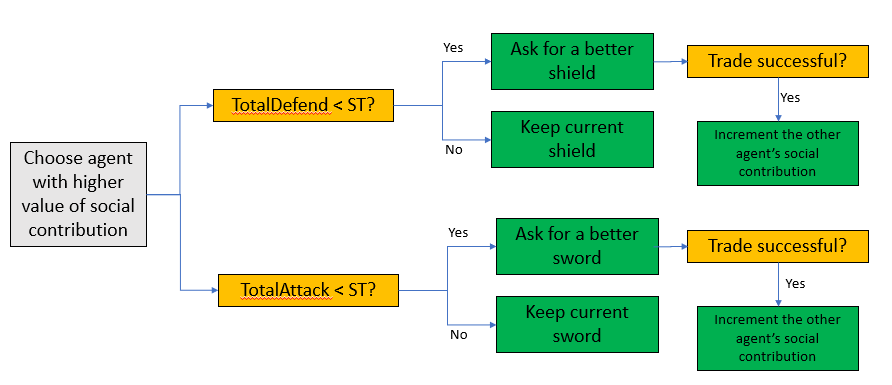
\includegraphics[width=0.5\textwidth]{007_team_4_agent_design/figures/4_trading_make.png}
    \caption{Trading structure for making requests.}
    \label{fig:proj_struct}
\end{figure}

\begin{figure}
    \centering
    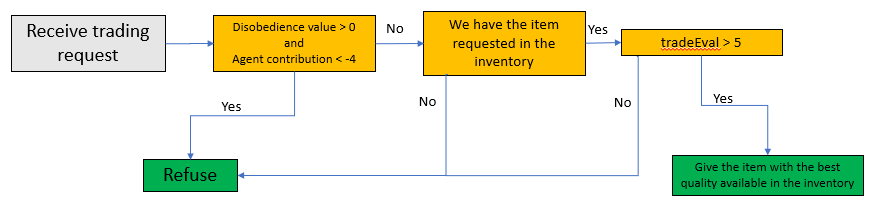
\includegraphics[width=0.5\textwidth]{007_team_4_agent_design/figures/3_trading_receive_2.png}
    \caption{Trading structure for receiving requests.}
    \label{fig:proj_struct}
\end{figure}

\subsection{Loot Distribution}

\par For the loot manifesto, the threshold of ST, HP, Attack and Defend are estimated with the same idea in the fight manifesto. If the agent's HP is smaller than the HP threshold (Equation 7.1), it is allowed to get a HP potion from the loot pool if there is one. Similarly, if its ST is smaller than the ST threshold (Equation 7.2), the agent is allowed to get a ST potion from the loot pool if there is one. Also, if both our HP and ST are greater than the HP and ST threshold, this means that our condition is good enough to fight and we should be equipped for that. Hence, we further analyse the TotalAttack and TotalDefend. If the TotalAttack is smaller than an Attack threshold, then the agent are allowed to get a sword from the loot pool in order to maximize the damage dealt to the monster. Similarly, if its TotalDefend is smaller than the Defend threshold, then then we are allowed to get a shield from the loot pool. We utilize the same voting mechanism in fight manifesto for the loot manifesto.

\par Last but not least, we are allowed to disobey the voted loot manifesto. If our HP is extremely low but our manifesto decision does not allocate us  getting a HP potion even there is one, we can simply get the HP potion and decrease our C at the same time. This case applies to ST potions as well. Figures 7.5 show the flowchart for deciding which item to get from the loot pool.

\begin{figure}
    \centering
    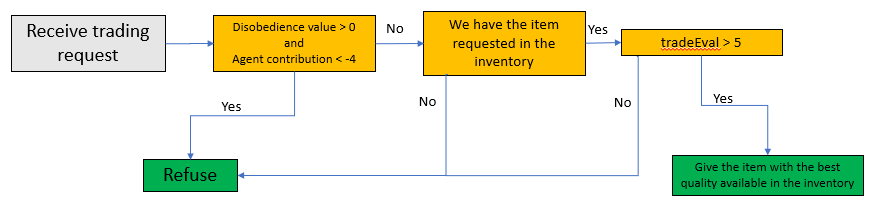
\includegraphics[width=0.5\textwidth]{007_team_4_agent_design/figures/3_trading_receive_2.png}
    \caption{Structure for loot distribution.}
    \label{fig:proj_struct}
\end{figure}

\subsection{Voting for Chair and Deposing}

\par The chair is voted in a simiFlar way that our agent votes for the manifestos and attempts to elect an agent that has a high social contribution rating and a similar governance plan than ours. Hence, if the candidate has (1) less or equal term length (2) similar number of necessary votes to depose (3) loot imposition (4) fight imposition and (5) a positive value of social contribution, we consider voting for that agent. If there is a tie, we will vote for the agent with the highest social contribution value (including our own agent).

\par As for deposing a chair, we analyse the ultimate result of this agent's administration that is, the number of agents killed during its term. If the number of agents alive have decreased 60\% since its election, we vote "YES" for deposing this agent from the chair. If the chair is deposed, its social contribution is decremented.



\subsection{Handling Disobedience}

\par The penalty for disobedience is to refuse all trading requests for a some period of time. Technically, each time an agent disobey, its disobedience value is incremented, and at the end of every 3 rounds, this value is decremented. This creates a mechanism of punishment by locking away those agents from trading with our agent. For instance, if an agent disobey the social contract, we don't accept trade requests with that agent for 3 rounds (until the disobedience value is decremented to 0). This also has a cumulative effect, so if an agent disobey twice in the same round, it gets a 6-round punishment, which may reinforce the importance of trusting the institution in power and and following social contracts. 

\section{Governance}
\par Our chair campaigns with the following manifesto: Number of levels - 10, Percentage of votes to depose: 65, Fight Imposition - Yes, Loot Imposition - Yes. Based on our governance strategy below, the actions of the agents may require  a few levels to reach the ideal results, as such our agent is campaigning to be in power for many levels. However, in the event that most agents do not want a chair for too long, we capped his/her term at 10 levels. The decisions to utilize a fight and loot imposition will be discussed below.
 
 \par The focus behind creating an apt system of governance, is how the knowledge of this elected chair is managed. Our governance is primarily based on an economy of esteem, which is a system that rewards agents who act in a manner that contributes to the progress of the group. This contribution is recognized in the form of attacking and defending, and the reward is in the form of a greater influence in voting on a proposal regarding fight and loot decisions. This is based upon the Athenian system of government in which greater cooperation and contribution to the collective resulted in greater social benefits. Our chair aggregates knowledge based on prior fight actions; we chose 3 prior rounds as this was long enough to assess patterns in agents’ behaviour but not so long as to prevent an agent from being able to change behaviour. Upon having the proposals from each agent, a weighted mean is taken of the thresholds for attacking, defending, and loot acquisitions, creating a new proposal. The weights of this mean are the number of votes an agent can have. Having fought (attacked or defended) 3 times in the past 3 rounds, gives an agent 4 votes, having fought twice gives 3 votes, having fought once gives 2 votes, and having fought 0 times gives 1 vote. The benefit of this approach is two-fold. Firstly, it incentivizes agents to contribute more to the collective good by rewarding them with a greater ability to make a choice. Secondly, given that an agent who has been fighting in the past few rounds has lower health, it gives them a greater voice to explain why they potentially deserve to rest in the form a cower decision. Once this new weighted proposal is created it is broadcasted to all agents to vote on it. If the vote does not pass, the weight of each category is decremented by one, except those of agents who did not fight at all in the past 3 rounds. This yields a proposal closer to the simple majority and then is broadcasted again, and the process repeats each time a vote does not pass. While simple majorities are not the best form of knowledge aggregation, the voting not passing multiple times suggests that the desire of the agents is closer to a simple majority than a weighted mean based around the collective good. As a result of creating and broadcasting a new proposal, our leader requires both the fight imposition and loot imposition.

\par Even in the case of a vote passing, certain agents are bound to be disobedient. Based on Ostrom’s 5th principle, there must be sanctions for those who disobey their expected action. However, our chair is not completely ruthless and is aware that very harsh punishments cause punished agents to resent the governance and the overall institution. As such, our chair only imposes sanctions in the form of reputation consequences by broadcasting, when an agent has disobeyed their assigned task, and how many times that agent has disobeyed. It is ultimately, up to each individual agent to decide how they want to deal with agents who disobey the chair.  

\section{Experiments and Discussion}


Experiment 1:
The first experiment was to analyze the performance of the game using set parameters. The parameters were 60 levels, starting health points of 1000, starting attack of 20, starting shield of 20, base stamina of 2000 and a threshold that 60\% of the agents must survive.
Figure 7.6 shows the results obtained by setting these parameters in the .env file of the repository. 

We can see that for the number of agents remaining at the end of each level, the line becomes quite consistent up to level 20. This means that we have 100 agents up to level 20 which shows strong performance under our agent strategy. The same pattern can be seen with the number of agents remaining at the end of each round. Up until round 67, the consistency of the line is very high showing that 100 agents have remained until round 67. However, it slowly starts to decline after this point where round 85 is left with 55 agents (game lost). 

The HP pool graph shows interesting trends where we see the HP pool gravitate upwards to 20,000 on level 4 (the maximum peak). However, it decreases after this point with no rise which indicates that agents stopped donating to the HP pool, by level 23 the agents start to constantly fight.

\newpage
\begin{figure}[htbp]
\begin{tabular}{ll}
    \centering
    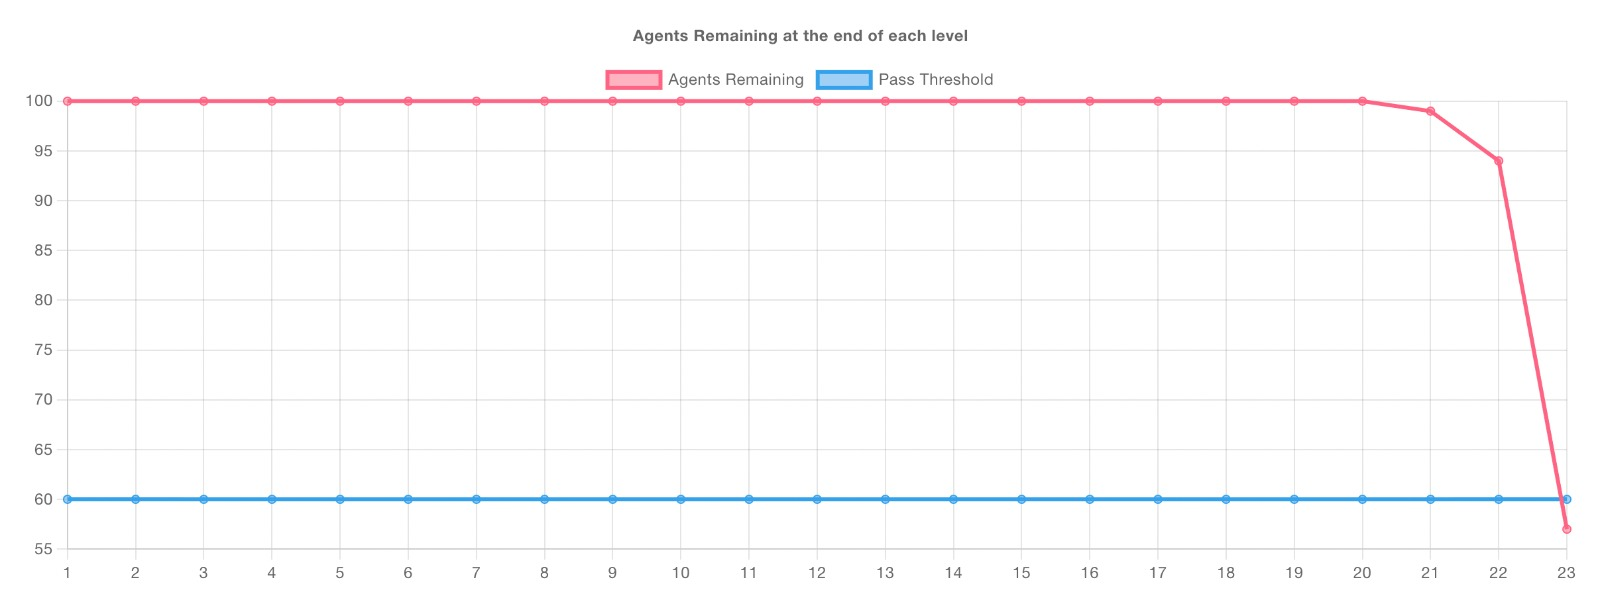
\includegraphics[width=0.5\textwidth]{007_team_4_agent_design/figures/EX1_1.jpg}
    &
    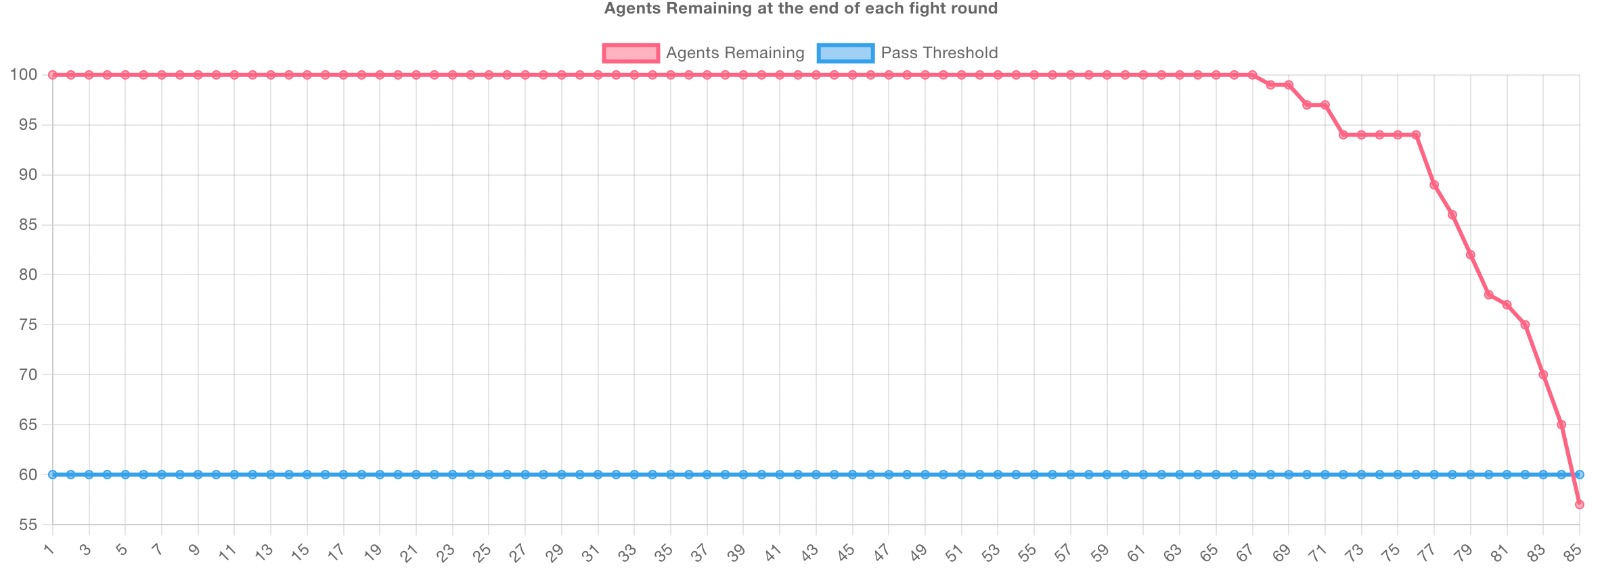
\includegraphics[width=0.5\textwidth]{007_team_4_agent_design/figures/EX1_2.jpg}
\end{tabular}

\end{figure}

\begin{figure}[htbp]
\begin{tabular}{ll}
    \centering
    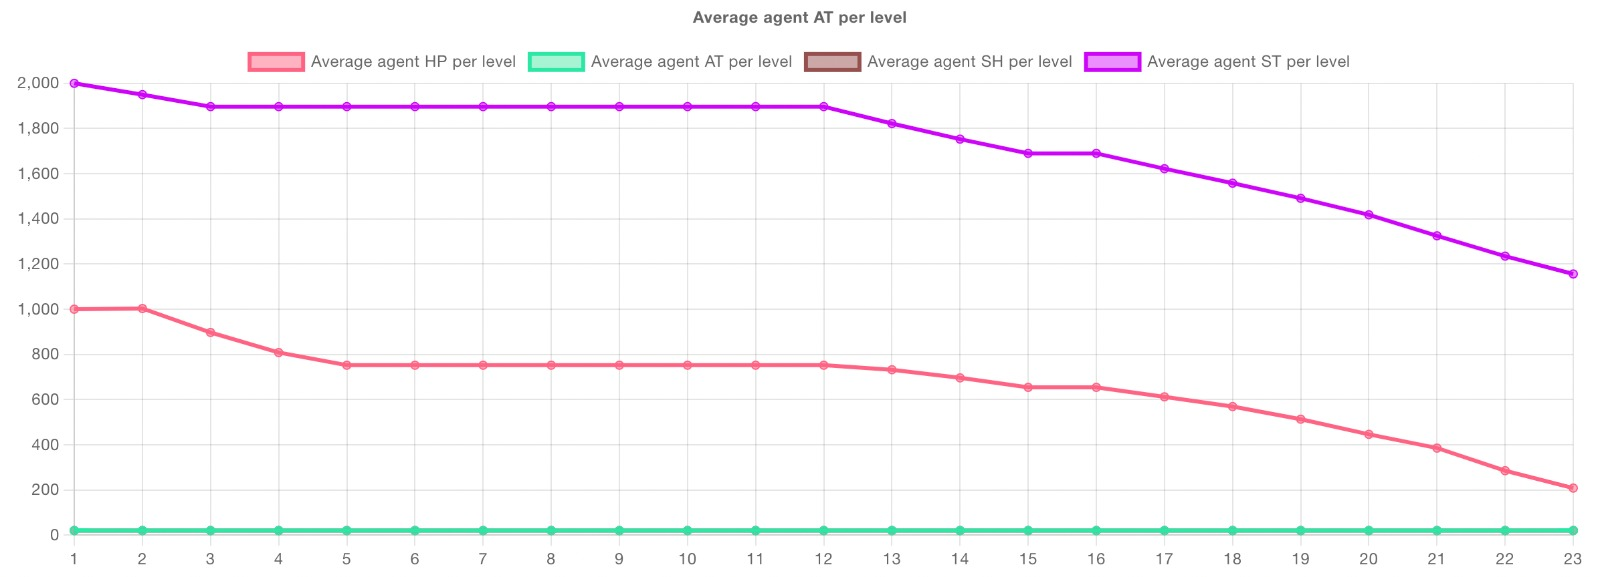
\includegraphics[width=0.5\textwidth]{007_team_4_agent_design/figures/EX1_3.jpg}
    &
    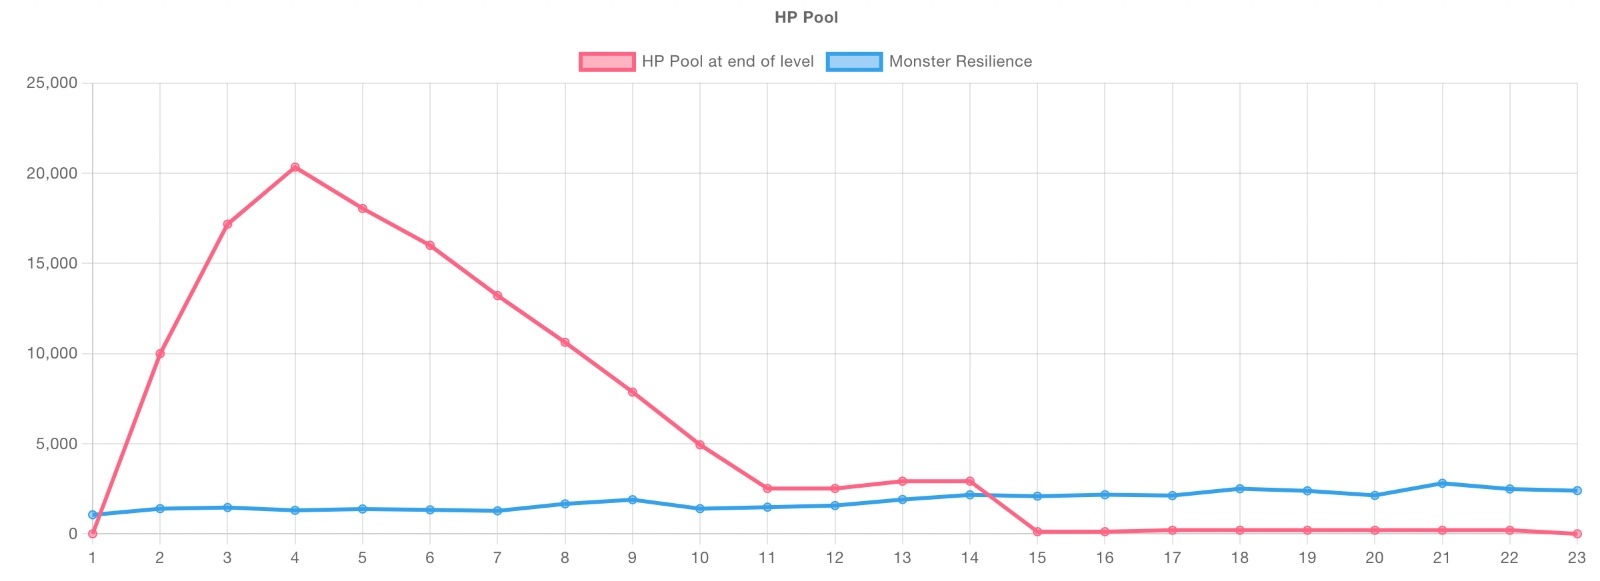
\includegraphics[width=0.5\textwidth]{007_team_4_agent_design/figures/EX1_4.jpg}
\end{tabular}
     
\end{figure}


\begin{figure}[htbp]
\begin{tabular}{ll}
    \centering
    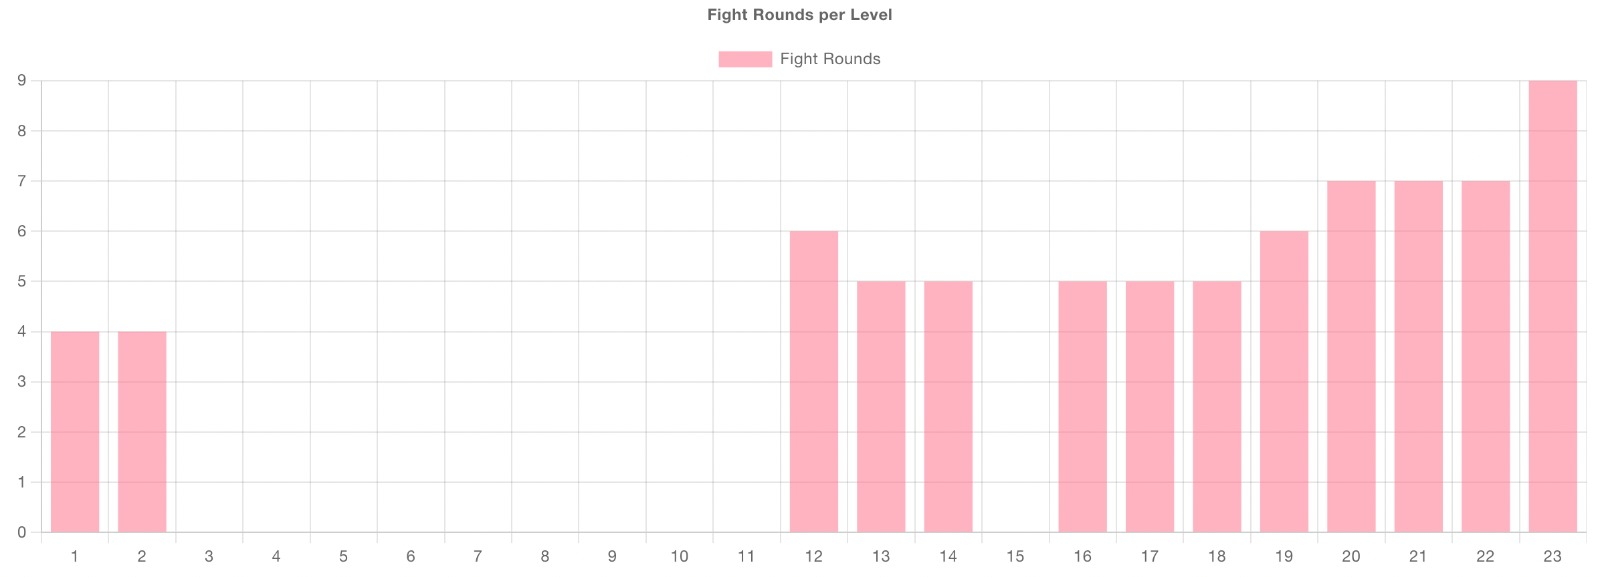
\includegraphics[width=0.5\textwidth]{007_team_4_agent_design/figures/EX1_5.jpg}
    &
    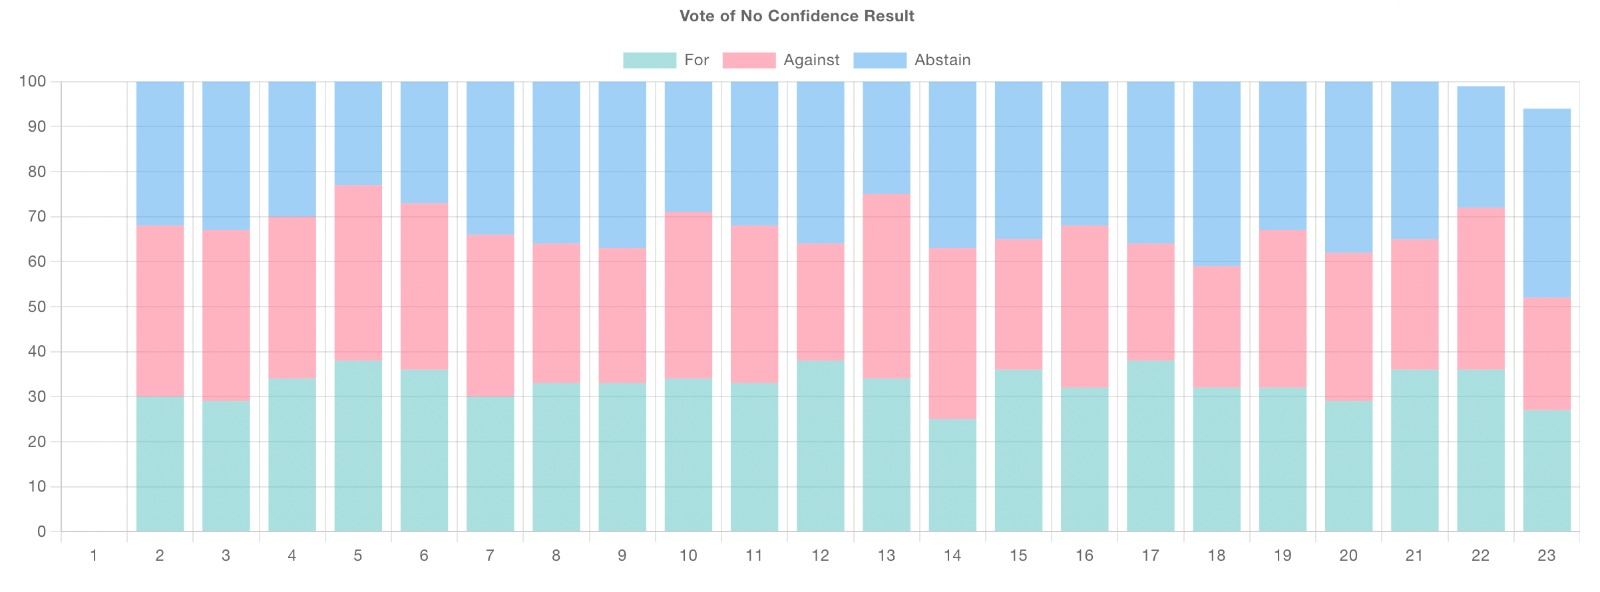
\includegraphics[width=0.5\textwidth]{007_team_4_agent_design/figures/EX1_6.jpg}
\end{tabular}
    \caption{Experiment results 1}
\end{figure}

\newpage

Experiment 2:
\par The parameters were now changed from 60 to 20 levels.

\begin{figure}[htbp]
\begin{tabular}{ll}
    \centering
    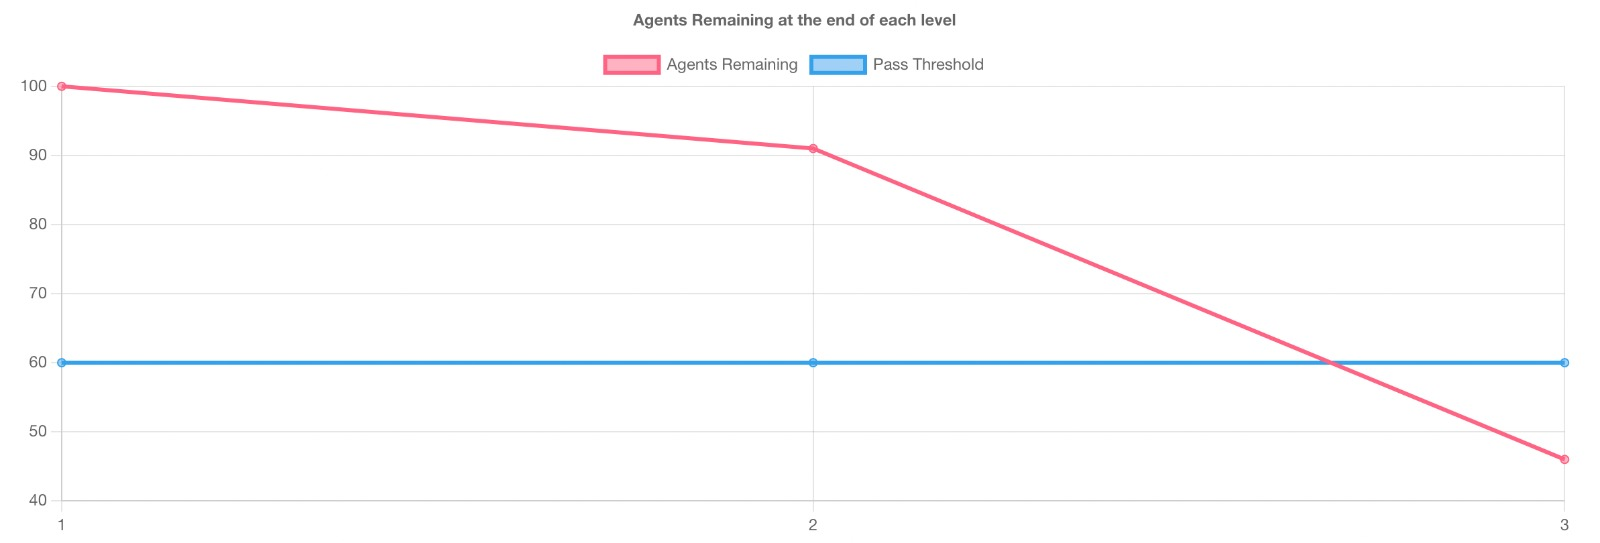
\includegraphics[width=0.5\textwidth]{007_team_4_agent_design/figures/EX2_1.jpg}
    &
    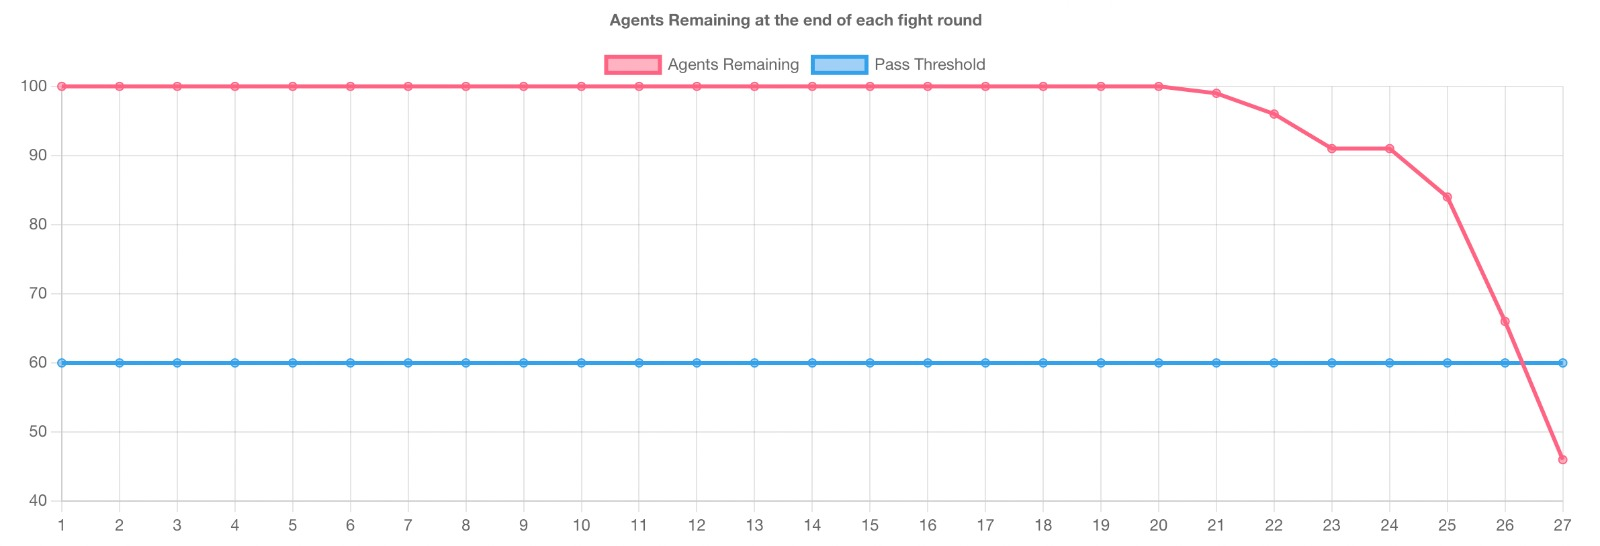
\includegraphics[width=0.5\textwidth]{007_team_4_agent_design/figures/EX2_2.jpg}
\end{tabular}

\end{figure}

\begin{figure}[htbp]
\begin{tabular}{ll}
    \centering
    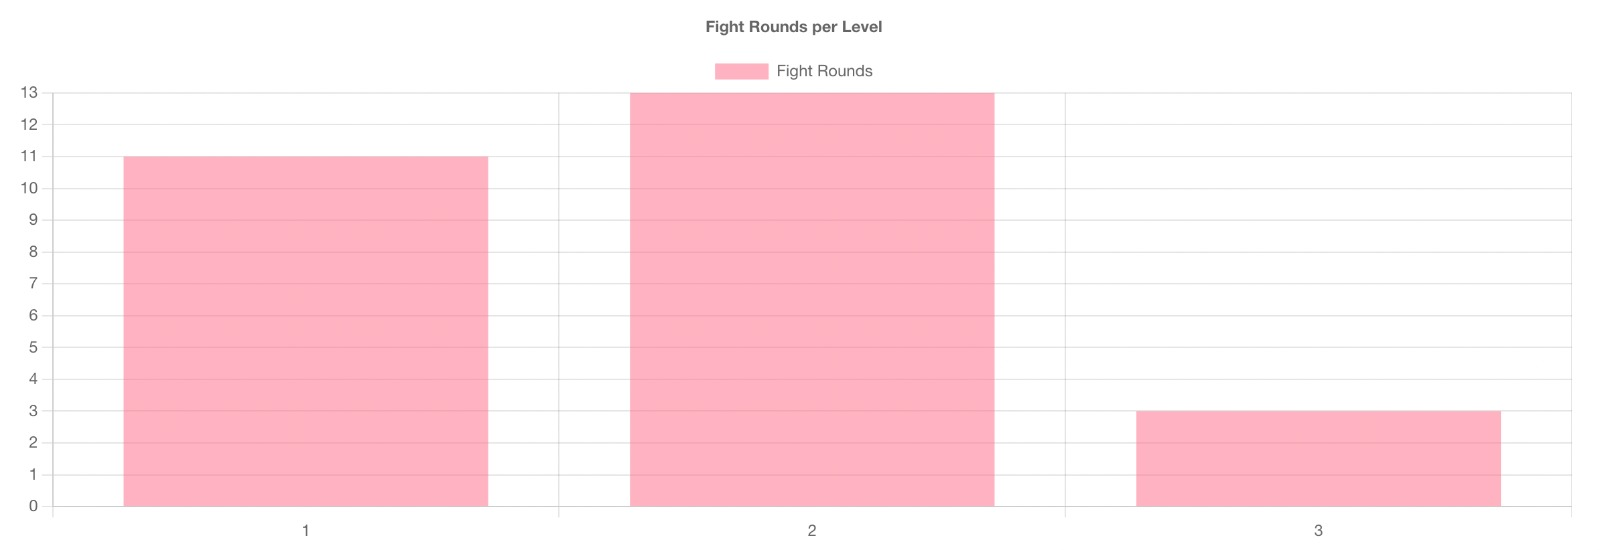
\includegraphics[width=0.5\textwidth]{007_team_4_agent_design/figures/EX2_3.jpg}
    &
    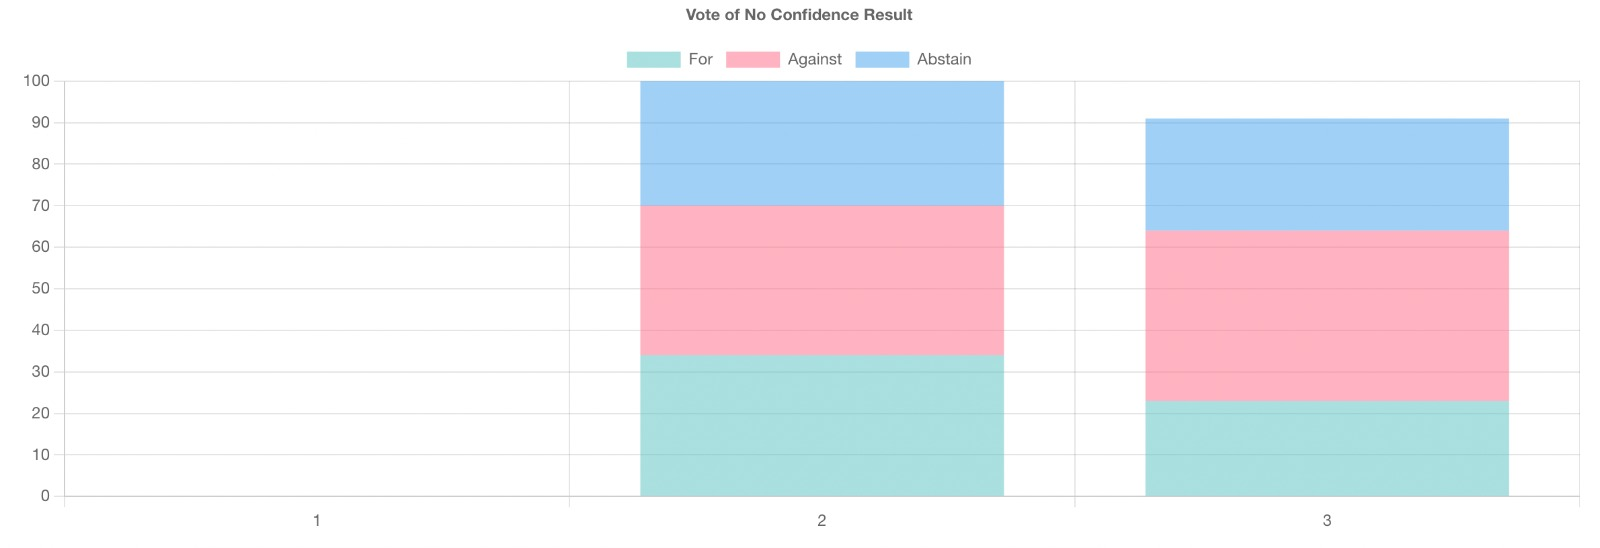
\includegraphics[width=0.5\textwidth]{007_team_4_agent_design/figures/EX2_4.jpg}
\end{tabular}

\end{figure}


\begin{figure}[htbp]
\begin{tabular}{ll}
    \centering
    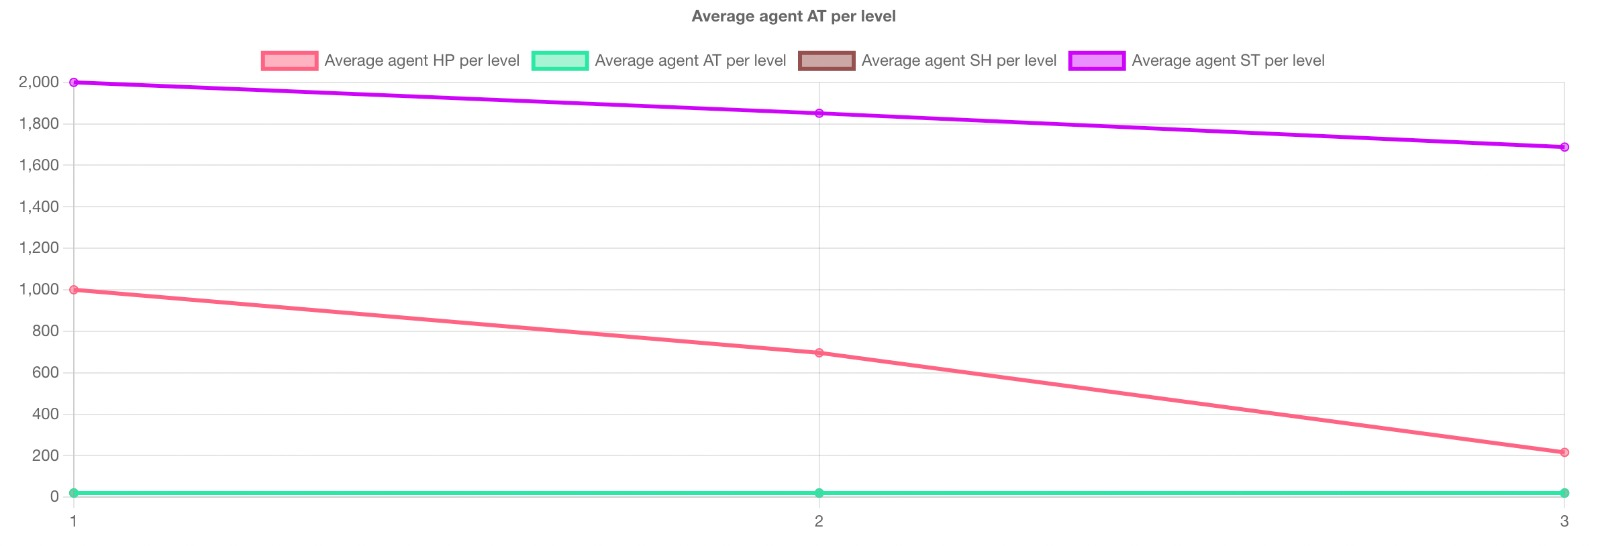
\includegraphics[width=0.5\textwidth]{007_team_4_agent_design/figures/EX2_5.jpg}
    &
    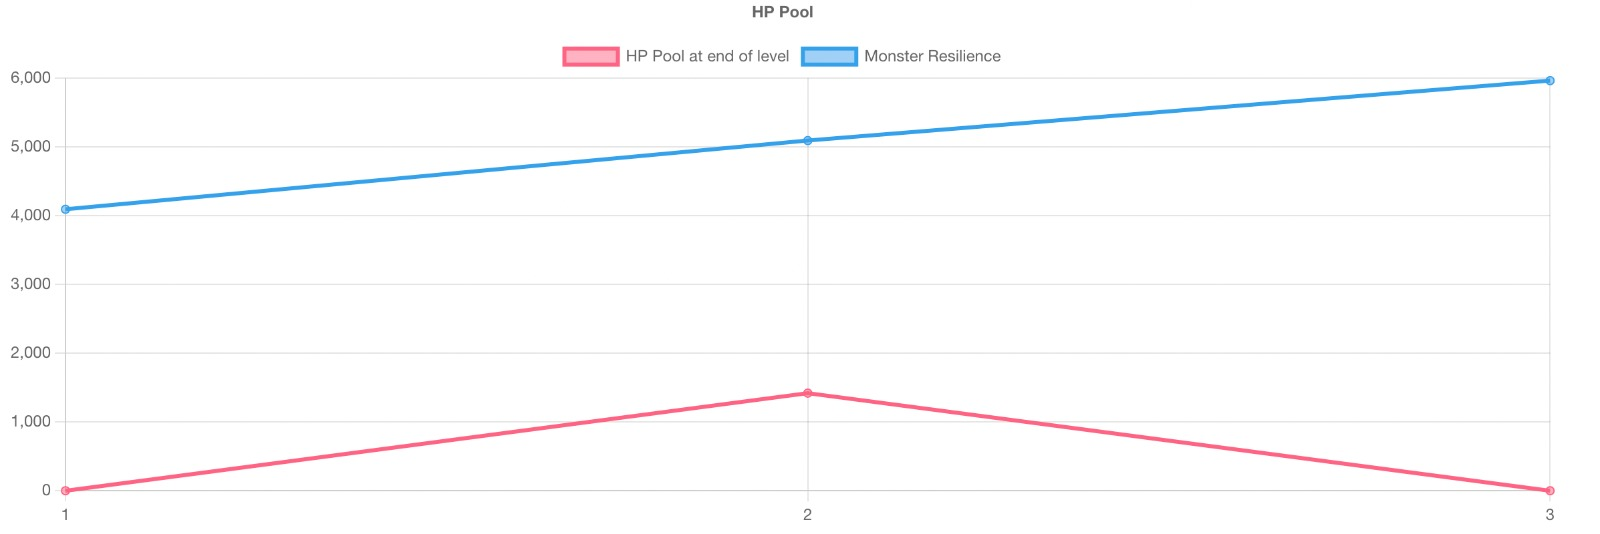
\includegraphics[width=0.5\textwidth]{007_team_4_agent_design/figures/EX2_6.jpg}
\end{tabular}
    \caption{Experiment results 2}
\end{figure}


\newpage

Experiment 3:

\par In the agents remaining at the end of each level graph the pass threshold is 18 and the agent remaining is 30, after 23 iterations we can see the agent remaining significantly declines and reaches its minimum at 

\begin{figure}[htbp]
\begin{tabular}{ll}
    \centering
    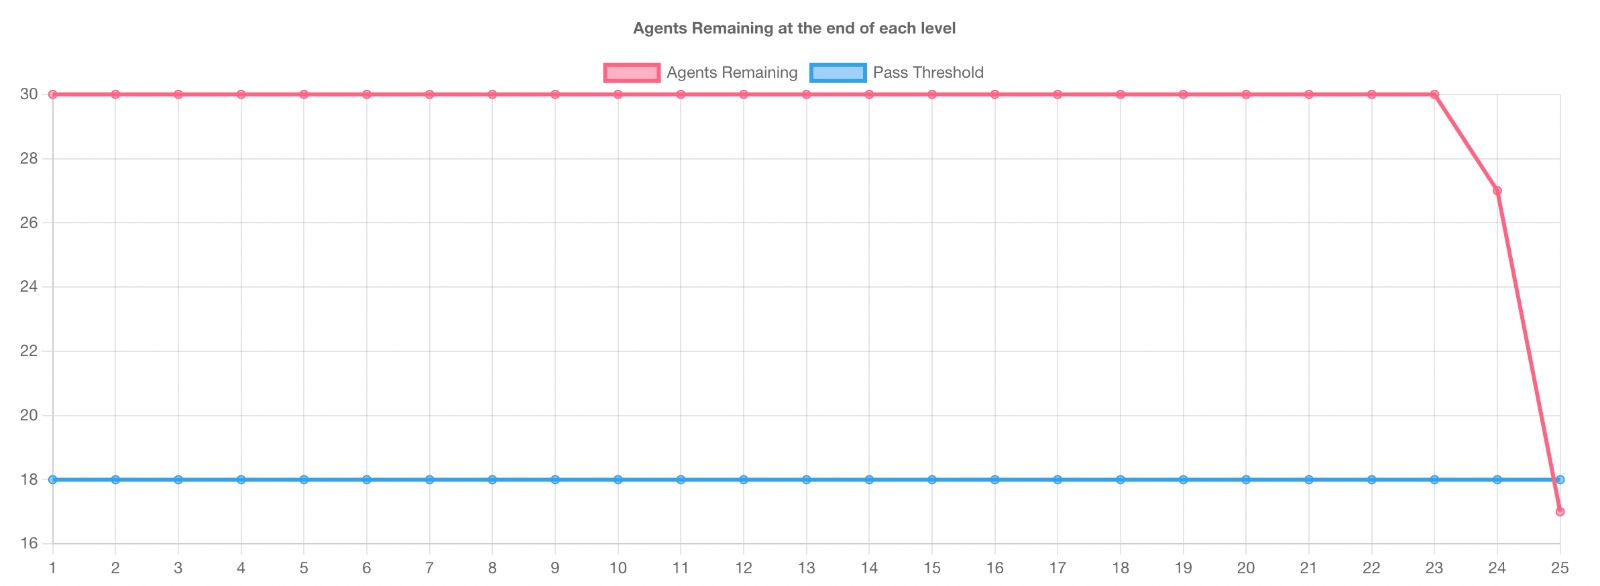
\includegraphics[width=0.5\textwidth]{007_team_4_agent_design/figures/EX3_1.jpg}
    &
    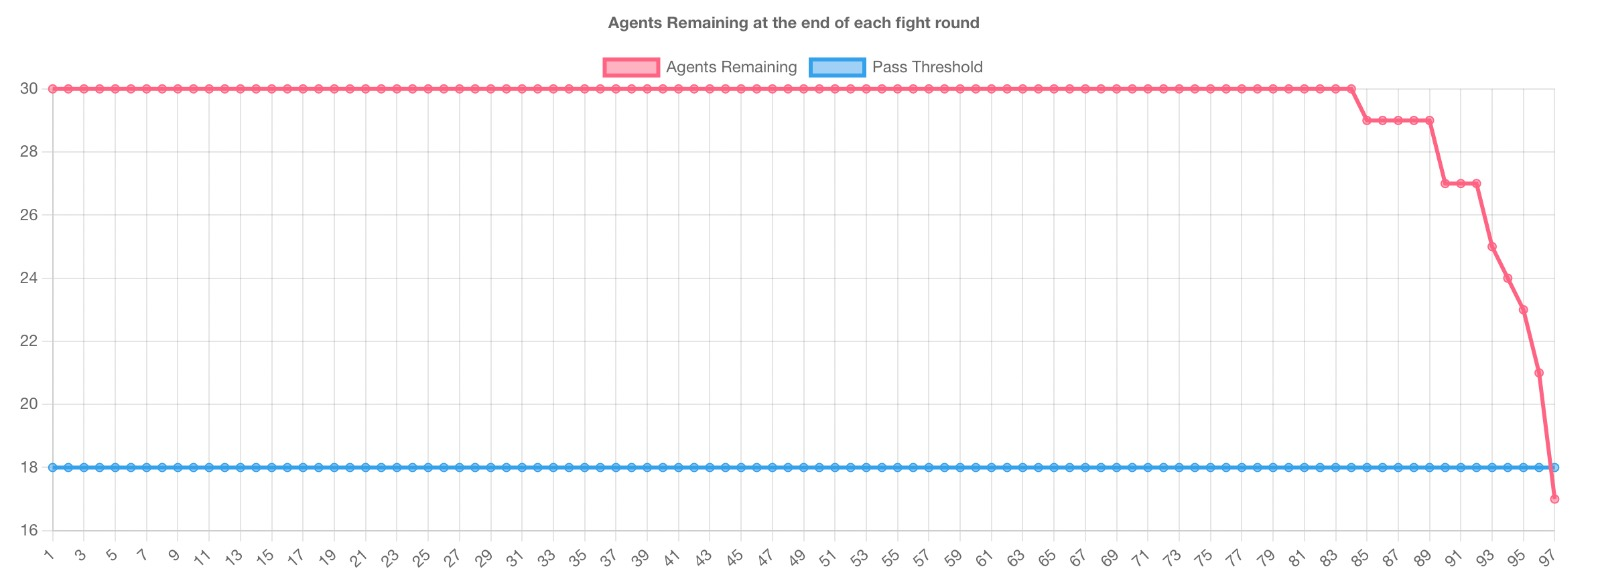
\includegraphics[width=0.5\textwidth]{007_team_4_agent_design/figures/EX3_2.jpg}
\end{tabular}

\end{figure}

\begin{figure}[htbp]
\begin{tabular}{ll}
    \centering
    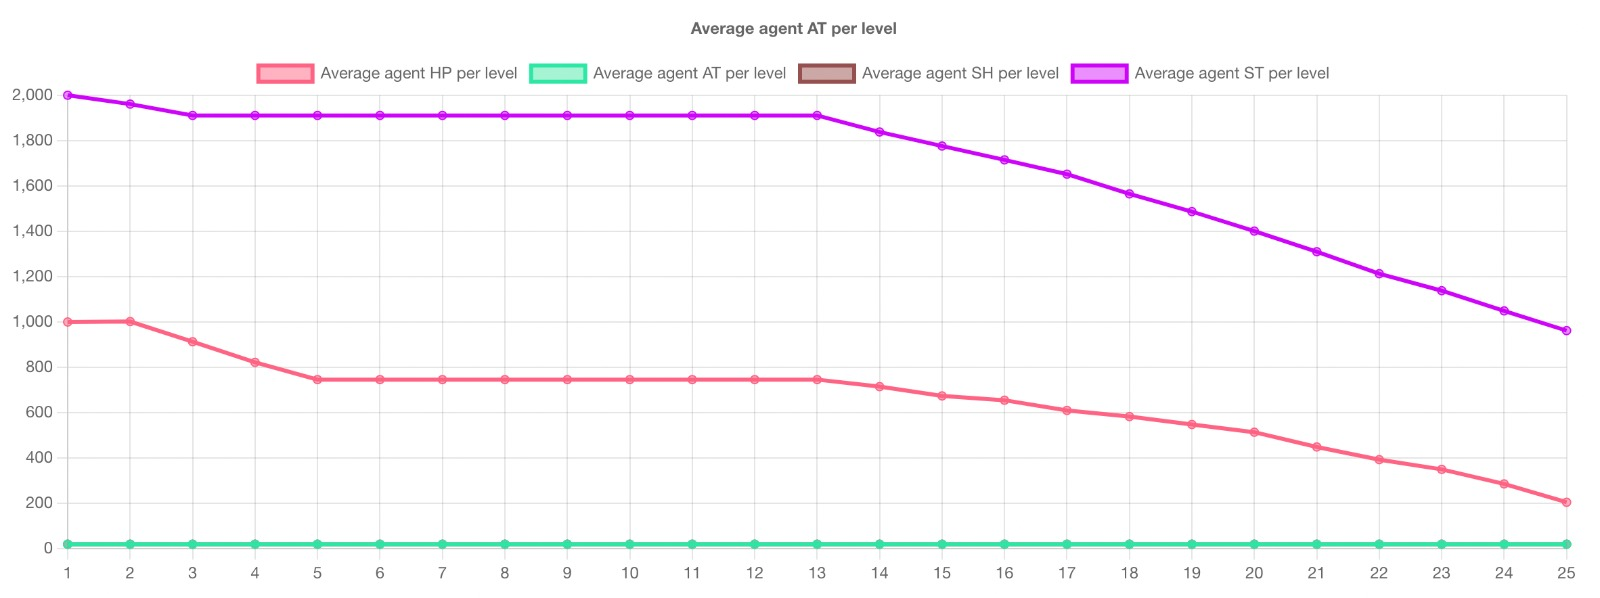
\includegraphics[width=0.5\textwidth]{007_team_4_agent_design/figures/EX3_3.jpg}
    &
    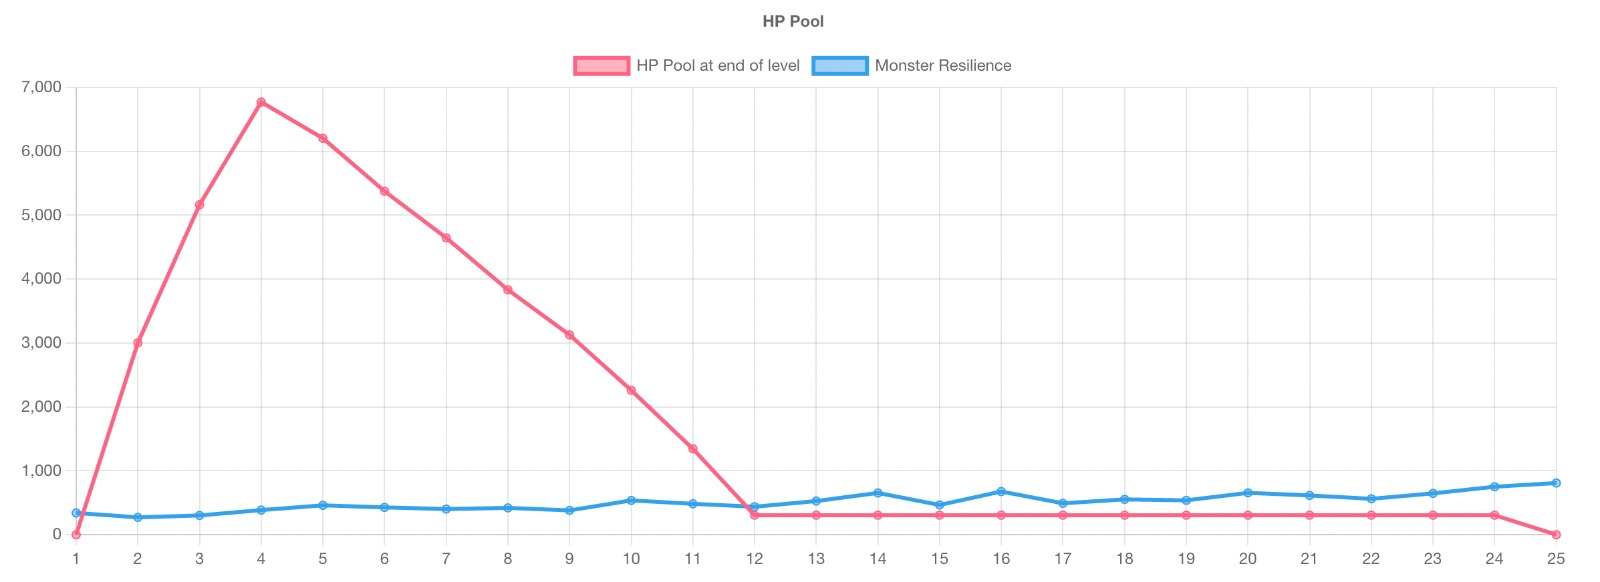
\includegraphics[width=0.5\textwidth]{007_team_4_agent_design/figures/EX3_4.jpg}
\end{tabular}

\end{figure}


\begin{figure}[htbp]
\begin{tabular}{ll}
    \centering
    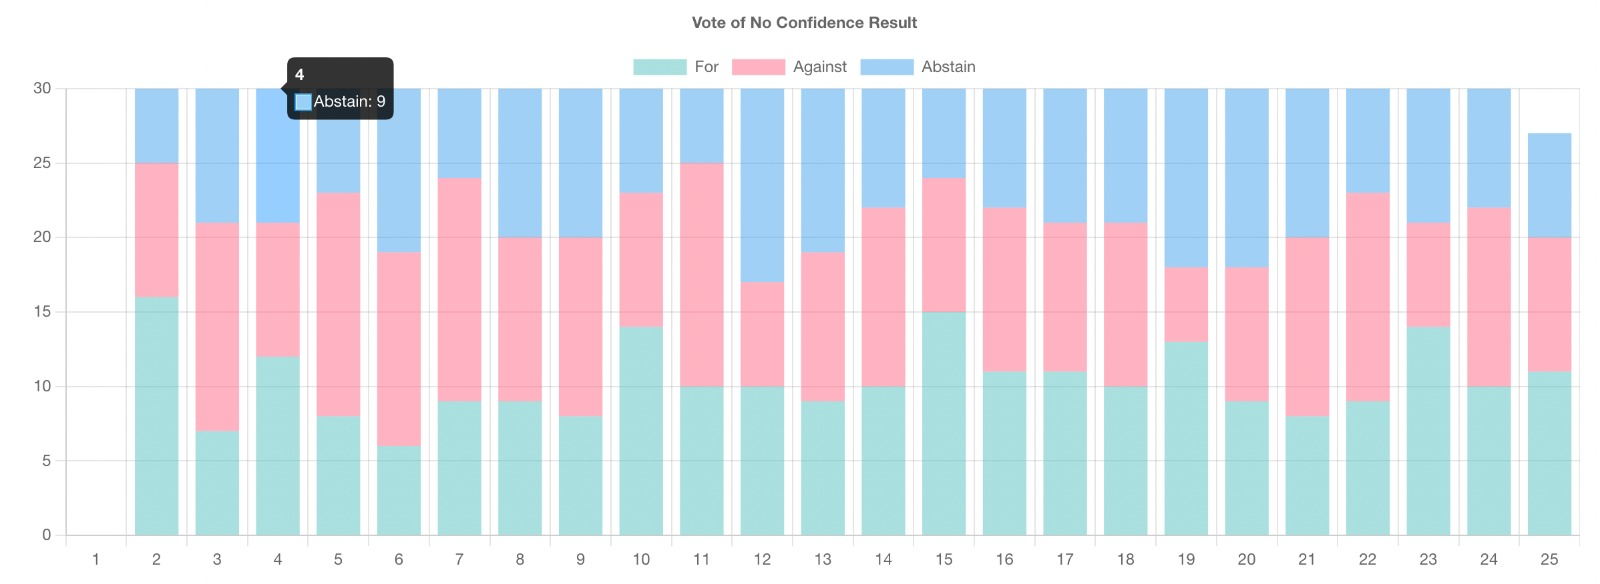
\includegraphics[width=0.5\textwidth]{007_team_4_agent_design/figures/EX3_5.jpg}
    &
    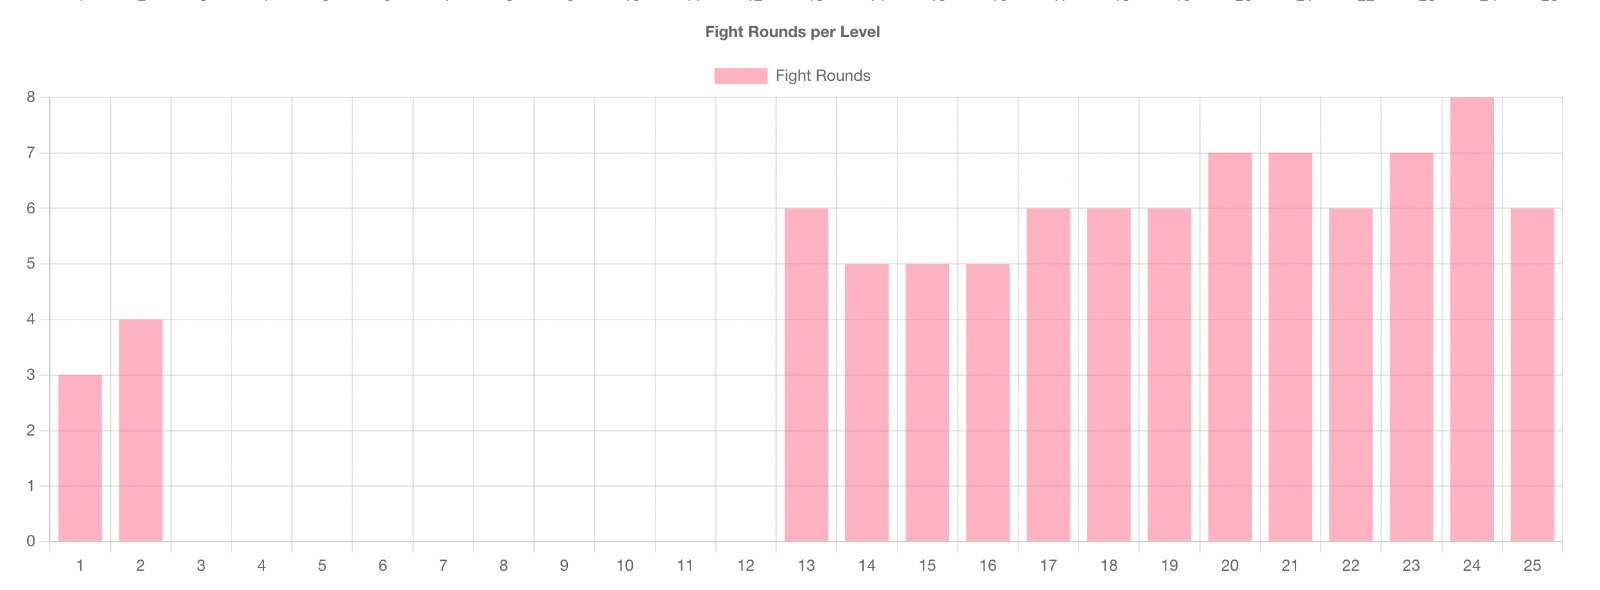
\includegraphics[width=0.5\textwidth]{007_team_4_agent_design/figures/EX3_6.jpg}
\end{tabular}
    \caption{Experiment results 3}
\end{figure}

\newpage

\par The key idea in our agent implementation is that it attempts to balance its social contribution and its chances of survival (economy of esteem). For instance, when reaching an impasse with the fight decision, our agent follows the logical decision for the common good more frequently. Also, it chooses to interact/trade with agents with a higher social contribution value and do not disobey social contracts, which reinforces the ideology implemented. Also, by donating to the HP pool, we can see how beneficial itwas in the simulations, since as soon as the agents start fighting the monster, they start to encounter difficulties and were not able to win the game. This reveals that contribution to social good yields better results than a selfish mindset.

\par By analysing the experiments 1 and 3 (60 levels) we can notice that our agent performs better than the random agent (survives until level 18). One of the reasons for that is our agent takes into consideration past actions from other agents in order to make a decision. With this learning process, our agent surpasses the random agent performance by replacing randomness for knowledge when making a decision. Also, in our agent's strategy, for the fight manifesto, the majority of agents fighting will be attacking since too many agents defending may lead to a prolonged level and a lot of damage being taken. Furthermore, our manifesto for loot distribution is based on each agent's current needs, which is an attempt to optimise the stats for each agent before the new level starts. Finally, we have a governance ideology that rewards agents that contribute to the social good, giving them more importance in voting.


\par It is valid to mention that our initial strategy included interactions with other agents before deciding our fight action. Essentially, it would ask other agents for their actions and take their responses into consideration to estimate how many agents would fight or cower. Unfortunately, this was not implemented since the infrastructure to make this communication possible was not completed. Therefore, the agent strategy that we wanted to implement was based on pre-fight communications which consisted on storing all the agent fight decisions (not just manifesto decisions) from the beginning to the end of the game. This would allow our agent to use predictive learning to past actions as a method to predict future actions which would optimize our chances of choosing better actions through prediction. Based on a given condition, the action of that particular agent would be stored until it iteratively goes through each agent action until the game is done.

\section{Future Steps}

\par Given the opportunity to better our agent, there are a few changes we would make to its design. One is the existence of a clear reputation framework. While different agents have abilities to assess their opinions of agents in the form of the social contribution (C), the existence of a standardized framework in which all agents can express their opinions on other agents and send these views to the chair would allow for a more robust economy of esteem. This would allow agents to make connections with other agents, and identify their reputation based on their fight decisions, amounts of trading, and interactions with other agents. The weights of these connections would change based on how often agents communicated which would relay to the chair how valid an opinion of another agent might be. 

%------------------------------------------------------------------end


\chapter{Team 5 Agent Design}\label{team_5_agent_design}

{\section[Overview]{Overview\\ {Our Actions and Goals towards the Common Goal}}}

\subsection{Leadership}
When voted leader with fight power our agent practices utilitarianism \cite{pitt} and promotes actions that maximises utility and wellbeing of all agents. For Escape the Dark Pitt, the collective aim is to defeat monsters and clear all levels with remaining population above 60 percent. Hence, we can derive utility being inversely related to damage received by agents and deaths. By prioritising decisions which will bring upon the greatest utility overall even at his own risk and having a selfless concern for other agents, our agent can also be deemed altruistic. But as completing the game is in our agent's self-interest, it is not pure altruism.

After each monster is defeated, a loot pool is dropped. We believe the loot pool is similar to a Common Pool Resource. All agents have equal opportunities to request for items, deeming the loot pool non-excludable. After an item has been allocated, it is unavailable to other agents, hence the loot pool is also rivalrous in consumption in line with Common Pool Resources. The main difference between the two is the loot pool can be fully depleted each round and fully replenished at the next, while common pool resources generally won't replenish if it is fully depleted. During loot allocation our agent utilises theory from equity and desert \cite{pitt} to aim for fairness and distributive justice by having each agent's allocation affected by their contribution. Unlike the health points pool, another common pool resource, agents cannot directly contribute to it. We can determine an agent's contribution by their fight decision as defeating the monster will drop loot, and in turn contribute to the loot pool. Fight decision along with other factors are used to calculate a social network score which will directly impact an agent's ability to be allocated resources per our algorithm.

\subsection{Collective Intelligence}

\begin{figure}[h]
    \centering
    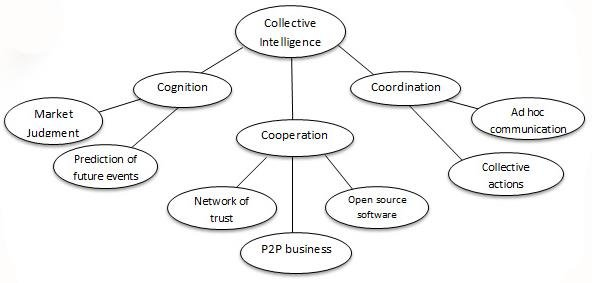
\includegraphics[width=0.63\textwidth]{008_team_5_agent_design/images/Collective-Intelligence-Branches.jpg}
    \caption{Collective Intelligence Branch}
    \label{fig:CQ}
\end{figure}

As an altruistic agent practicing utilitarianism, our agent aims to improve collective benefit through our own judgement. One way of doing so is to encourage the growth of collective intelligence. Where collective intelligence can be obtained from and have an impact on the following three fields: cognition, corporation, and coordination. We adapt \ref{fig:CQ} \cite{rescher1966} to this game scenario as follows:

\begin{itemize}
    \item Cognition
          \begin{itemize}
              \item Perspectives
                    \begin{itemize}
                        \item Every agent's perspective on their own status and overall situation - whether they know if they are a popular leader, a helpful peer to the situation, etc. It can be observed from leader status (winning leader election, finishing the leader's term without being overthrown, overthrown). How the majority of other agents are in the social network map, i.e. if only a few agents have a low social network profile, we can deduce that those agents are not welcomed; but if the majority of agents are in a low social network profile, it may be the case that our agent is actually the one that is not welcomed.

                        \item Every agent's perspective on other agents can be observed from interaction and information, for example, fight decision (fight intention, defect), proposals,
                        \item Perspective to the environment - agents may over-estimate or under-estimate the monster and the loot market.
                    \end{itemize}
              \item Interpretation of the common goal

                    Agents can interpret the common goal and make up their own beliefs in different ways. For example, agents may determine the spectrum between altruism and selfishness to be the best strategy of achieving the goal with understanding and deduction.
          \end{itemize}
    \item Cooperation
          \begin{itemize}
              \item Social Network

                    In the cooperation process, every agent can gain knowledge of other agents to form an opinion and decide their future interactions. There exists an underlying social network that connects the agent's communication and interaction in some ways. By discovering this social network our agent can make more effective interactions with other agents.
              \item P2P interactions

                    With the existence of the social Network, it can impact the social distance of each P2P interaction, in this case, how likely to send a trading message and how likely to mutually agree on a negotiation.
          \end{itemize}
    \item Coordination
          \begin{itemize}
              \item Collective action

                    With a common goal, agents can self organise to collectively move towards the goal in some way. Each agent's contribution can have an impact on the whole cohort, voting for example. Individual intelligence is the base of collective intelligence as well as how individual intelligence coordinates. With the leader mechanism and communication mechanism in this game, it gives more opportunities to form collective intelligence through coordination interactions.
          \end{itemize}
\end{itemize}

\subsection{Trade}

Our trade strategy extends the Agent's utilitarian approach and altruistic personality to achieving the collective aim. With this in mind, there is no significance in the weapon or shield we equip if the game is lost. Hence, no concern is given towards the weapon or shield equipped when finally escaping the pit. As each agent has an equal opportunity of receiving loot if they chose to fight, the exclusivity of shields and weapons are low. As we have no concern of our final equipped shield or weapon, the allocation of loot (consumption) to other agents will not subtract from our utility, deeming subtractability to be low. This in turn means that trading is not seen as a common pool resource problem.

On the contrary, other agents may value their weapon and shield equipped at the end of the game. In other words, trading will benefit other agents as weapon and shield statistics are valued, so the subtractability of weapons and shields would greatly increase in their perspective.

Considering agent's fight decision as their contribution towards loot, and by coupling trading with fight decision, we can frame this as a common pool resource problem. The common pool resource is sustained through defeating monsters with increasing difficulty to drop new and better items. Our agent takes advantage of this observation and rewards agents with regards to their contribution.


\section{Social Network}

\begin{itemize}
    \item Social Network Motivation
          \begin{flushleft}
              \setlength{\parindent}{2em}
              Since the agents are connected, interaction and impact can be made to other agents, therefore mapping and recording a social network can help our agent optimise the interaction outcome by going to the right agent. Social networks can also spot conflict in a system and help our agent identify its own position in the system. At last, due to this game's nature, an agent has limited scope to collect information meanwhile needs to make multiple multi-dimensional proposals and decisions as its prediction of optimal, however not long enough game duration is available to collect experience (plus the game can end early if agents fail), due to constraints, for the most of the time, an agent can only be trained with solo-play, duplicates of itself or random agents. Machine learning heavily based model is data-hungry, and risk overfitting to it self's characteristic, making it less robust in heterogeneous environments. We can make a trust system in the social network to estimate the reliability of another agent. Therefore utilising other agents' experience(that is visible to our agent) as a source of information for our soft-coded rule-based agent is effective for individual intelligence growth. A vivid example of connection and social networks that improve efficiency is that knowing the previous SOMAS class work out that GoLang is a suitable language for this coursework and has gone down with GoLang for two years in a row, our cohort has decided to rely on intuitively trust the previous SOMAS classes and save effort by relying on their experience, even though by the course no one had experience in GoLang before.

          \end{flushleft}
    \item Social Network Construction
          \begin{itemize}
              \item  Our Scope - where social network trust scores can update upon

                    There are two main fields that our agents can scope into to make and record their observations, interaction, and information, interaction is where arbitrary messages and decisions flow between two agents, while information is the one-way observation of our agents to other agents' visible states or their other behaviours. Interaction scope includes their trading process with us and their communication with us. Information scope includes their agent states, their votes, proposals, and defect status.
              \item Our Perspective
                    \begin{itemize}
                        \item Forming perspective

                              Once our agent has the observations, it uses its belief to form its perspective based on its observations. It parses the observations into two trust scores, strategy score and goodwill score, reference to our agent of how much can it trust another agent's strategy-related interaction and goodwill-related interaction. the history of another agent's past social network profiles is also one of the parameters to form new perspective.

                        \item Soft-coded boundary rules

                              Our agent reflex on itself based on the agent system's performance, then decides whether there is a need to modify its rules to be more helpful to the system. The personality classification boundaries are constant, but by applying scaling to agents' trust scores, the boundaries can also be viewed as a varying factor on a reverse to the scaling.
                        \item Forgiveness

                              "In social systems, forgiveness allows the truster (victim of the violation) to distinguish between intentional and unintentional violations (and a range of infractions in between)" \cite{pitt}. Forgiveness also helps the system restore stability. We chose very simple forgiveness by simply adding a recency bias to past history profile, time soothes the scar.
                    \end{itemize}
              \item Our intelligence

                    By collecting and digesting as much information from inside and outside of our agent, and with experience increase, our agent grows the intelligence that allows it to act more effectively to help the collective reaching the goal. It converts its obtained knowledge into intelligence. The knowledge can be distinguished as Knowledge of the environment, i.e. how much damage we receive and how much loot we gain, how many agents, and our estimation of their resources lost when agents interact with the environment. Knowledge of other agents, which is the perspective of them that our agent formed.  The advantage of this process is that our agent becomes giving more and more reliable predictions of optimal next-move decisions.
          \end{itemize}

    \item Social Network Function

          The implementation and exploitation of personalities and trust scores can be found in \ref{fig:Information2Trusts} and \ref{table:personality_impact}

    \item Social Network - Information - our scope and observation

          The agent's strategy trust score and goodwill trust score are both in the range of [0,1], and both are initialised at 0.5. If during an update of trusts, their maximum variation in a trust exceeds 1, that trust score will be scaled by the max-min method.
    \item Social Network - Interaction - our exploitation of the trusts

          In order to save computational complexity, a personality perspective is formed by parsing trust scores. with both the upper boundary at 0.8 and the lower boundary at 0.2, the trusts are quantised and categorised into 3 goodwill personalities of {good, goodwill\_neutral, evil} and 3 strategy personalities of {lawful, strategy\_neutral, chaotic}. The two sets of personalities can be combined to map a 2-D in total 9 personalities.

\end{itemize}

We don't want to exclude one's excellence in one field due to short comes in an irrelevant fields.

Here we have agents' algorithm for their fight strategy and the algorithm for their leader duties' functionality potentially written differently.

Hence, we establish two different trusts, which can decouple an agent's strategy quality and leadership goodness. This does not mean the trusts are completely independent, there are still common factors for both of the trusts.The irrelevant features are excluded from one to another.

The agent uses these trusts to summaries features from the left-hand side and contributes to the decision-making of the right-hand side.

Due to the limited size of the game and size of the features, it is sensible to summaries this 2-D personality based on two trust scores

The boundaries for the trust scores are both at $0.2$ and $0.8$ and initial scores at $0.5$, all of the agents will be True Neutral agents at the beginning and will be the majority for most of the game time. When developing the logic, True Neutral agents are included in all of the interactions, although priority will be given to some other personalities, but,
\begin{enumerate}
    \item The prioritised agents are small amount due to a high standards therefore to make sure there is still the majority of the resource that is left with the bigger amount of agents
    \item The accumulated trust addition in a level is less than $0.2$ for each of the scores, therefore it will take at least 2 levels for an agent to gain a personality with priority, which ensures enough interaction has happened or enough information is gained for the agent that we can make a new judgment to its personality. When updating the trust, if there is a trust score exceeding the region of 0-1, the max-min scale is applied to all agents. Under this circumstance, there will be at least one min-scored agent and one max-scored agent that has two different personalities that are not neutral.
\end{enumerate}

\begin{figure}[htb]
    \centering
    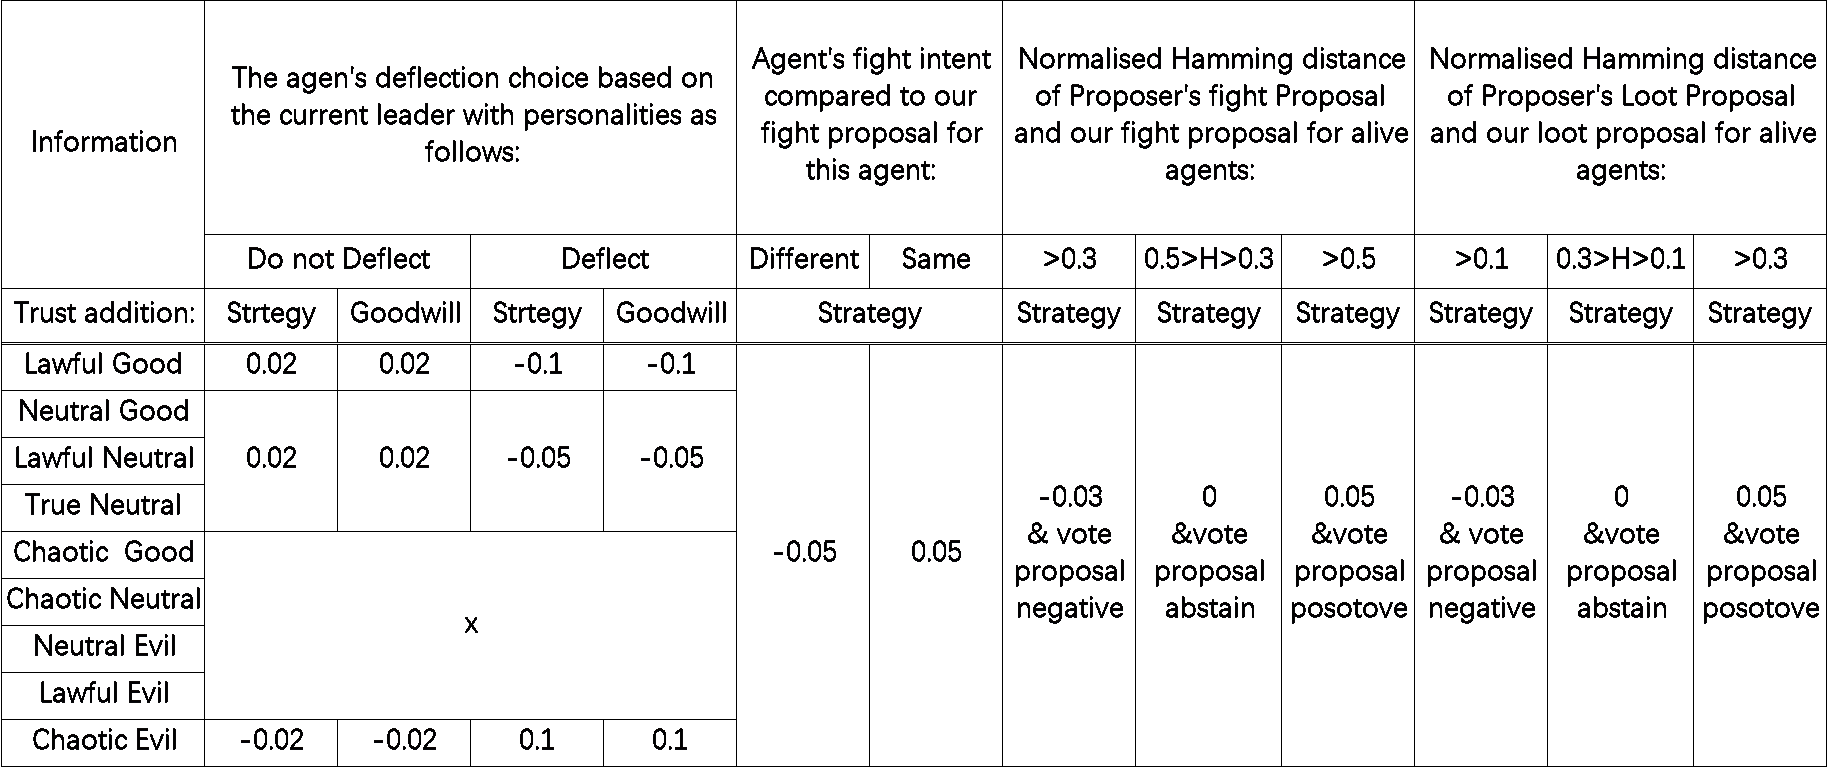
\includegraphics[width=0.95\textwidth]{008_team_5_agent_design/images/Information2Trusts-sideway.png}
    \caption{Details of updating trusts regarding different information that can be collected.}
    \label{fig:Information2Trusts}
\end{figure}

\begin{table}[htb]
    \centering
    \small
    \begin{tabular}{ |c|p{16em}|p{16em}| }
        \hline
        Interaction                       & Loot Resolution                                                                                                      & Loot Allocation Proposal                                                                                                                                                                                      \\
        \hline
        Explanation                       & Extract agents in a conflict with the highest ranked personality as follows and exclude the rest from this conflict. & Allocate the loot item with the highest value to the agents with the highest ranked personality. Once these gents each got an item, apply the same method to the rest of the loot and the rest of the agents. \\
        \hline
        \multirow{2}{*}{Other Conditions} & Fighting Item                                                                                                        & Recovery Item                                                                                                                                                                                                 \\
        \cline{2-3}
                                          & HP != LOW \&\& Stamina != LOW                                                                                        & HP == LOW \&\& Stamina == LOW                                                                                                                                                                                 \\
        \hline
        Lawful Good                       & \multicolumn{2}{c|}{1}                                                                                                                                                                                                                                                                                                               \\
        \hline
        Neutral Good                      & \multicolumn{2}{c|}{2}                                                                                                                                                                                                                                                                                                               \\
        \hline
        Lawful Neutral                    & \multicolumn{2}{c|}{3}                                                                                                                                                                                                                                                                                                               \\
        \hline
        True Neutral                      & \multicolumn{2}{c|}{4}                                                                                                                                                                                                                                                                                                               \\
        \hline
        Chaotic Good                      & \multicolumn{2}{c|}{5}                                                                                                                                                                                                                                                                                                               \\
        \hline
        Chaotic Neutral                   & \multicolumn{2}{c|}{6}                                                                                                                                                                                                                                                                                                               \\
        \hline
        Neutral Evil                      & \multicolumn{2}{c|}{7}                                                                                                                                                                                                                                                                                                               \\
        \hline
        Lawful Evil                       & \multicolumn{2}{c|}{8}                                                                                                                                                                                                                                                                                                               \\
        \hline
        Chaotic Evil                      & \multicolumn{2}{c|}{9}                                                                                                                                                                                                                                                                                                               \\
        \hline
    \end{tabular}
    \caption{Other agents' personality impact on our agent's interaction behaviour.}
    \label{table:personality_impact}
\end{table}

\pagebreak

\section{Manifesto}
\begin{itemize}
    \item Loot Power - Yes
    \item Fight Power - Yes
    \item Term Length -  1 level if haven't been elected before
          \begin{itemize}
              \item 2 levels if running the 2nd leader term
              \item 3 levels if running the 3rd leader term
              \item back to 1 level if overthrow happens in its last leader term, but wait until recency bias\^time is low
          \end{itemize}
    \item Overthrow Threshold - 50\%
\end{itemize}

\begin{itemize}
    \item Reflexive governance

          The agent reflex on its leadership quality and extend to all related algorithm and then can modify its coordinating strategy and corresponding cognition, based on knowing how well it has been as a leader. If the agent has made a leader, it can deduce that itself has a high reputation in other agents' inner states. If a leader has made to the whole term length, then it can gain confidence in its leadership ability, hence has the confidence to run for a longer term in the next time, which is more difficult because we presume it is less appealing than a shorter term manifesto to and need to have a even higher hidden reputation among other agents in order to win. If a leader has been overthrown, depending on its overthrown threshold, it loses its confidence of leadership possibly as well as some reputation, the way our agent reflex on being overthrown is to be humble of their leadership logic and start with running for 1 level of term length. Furthermore, this agent may want to rest for some time until the situation changed, its reputation is restored and it reflexively learned to refine its belief and rules, that it wants to rerun for leader again.
    \item Individual intelligence and Collective Intelligence via Education

          Being  a leader is not only empowered with extra impact to contribute to the system, but also enlarges the agent's scope. In this game, by being a leader can count the votes and has the ability to see every loot request message, which is not visible to a normal agent. By being a leader, if the agent opens entry to collect these information it can gain knowledge hence intelligence  faster. The reason of our agent's manifesto start with only 1 term length is for that the manifesto becomes more appealing to other candidates and hence more likely to become a leader to learn. By incrementing the term length once this agent has been raised to see further, it also want to leave more opportunity for agents that requesting less term length to also go to the leader position to be educated with the same vision our agent once had. Also by encouraging agents to run for leadership with shorter term length can increase the leader liquidity, hence more agents can become leaders once and have this "eye open" information collection opportunity. And the aim in the last is to increase collective intelligence.
    \item Individual Knowledge Diversity

          Continue to that we encourage leader liquidity, so that more agent can expose their coordinate logic as a leader. As a normal agent, experiencing more leaders in the same amount of time can let it know what coordinating logic are existing in the system, and diversify the choice of coordinating methods, which was originally each leader's own individual knowledge.
\end{itemize}

\section{Leadership}
\subsection{Leadership Personality}
When voted leader with fight power our agent practices utilitarianism \cite{pitt} and promotes actions that maximises utility and wellbeing of all agents. For Escape the Dark Pitt, the collective aim is to defeat monsters and clear all levels with remaining population above 60 percent. Hence, we can derive utility being inversely related to damage received by agents and deaths. By prioritising decisions which will bring upon the greatest utility overall even at his own risk and having a selfless concern for other agents, our agent can also be deemed altruistic. But as completing the game is in our agent's self-interest, it is not pure altruism.

After each monster is defeated, a loot pool is dropped. We believe the loot pool is similar to a Common Pool Resource. All agents have equal opportunities to request for items, deeming the loot pool non-excludable. After an item has been allocated, it is unavailable to other agents, hence the loot pool is also rivalrous in consumption in line with Common Pool Resources. The main difference between the two is the loot pool can be fully depleted each round and fully replenished at the next, while common pool resources generally won't replenish if it is fully depleted. During loot allocation our agent utilises theory from equity and desert \cite{pitt} to aim for fairness and distributive justice by having each agent's allocation affected by their contribution. Unlike the health points pool, another common pool resource, agents cannot directly contribute to it. We can determine an agent's contribution by their fight decision as defeating the monster will drop loot, and in turn contribute to the loot pool. Fight decision along with other factors are used to calculate a social network score which will directly impact an agent's ability to be allocated resources per our algorithm.

\subsection{Leader Fight Logic}
As mentioned in leadership personality, our agent aims to maximise utility by prioritising taking the least total damage and deaths when making fight decisions. There are 2 fighting conditions where the level can be passed without taking any damage or deaths. The leader fight algorithm will first check for the following two criterions:

\begin{enumerate}
    \item
          $\sum{\text{Agent Attack}} > \text{Monster Resilience}$

          If the sum of Agent's attack values is greater than monster resilience, we are capable of defeating the monster in one fight round without giving it the opportunity to deal damage.

    \item
          $\sum{\text{Agent Shield}} > \text{Monster Attack}$

          If the sum of Agent's shield values is greater than monster attack, we will receive no incoming damage.
\end{enumerate}

If either criterion is met, the fight decision is determined by minimising stamina consumption:

\begin{enumerate}
    \item  Agents are ranked according to their attack values. The agent's attack values are summed iteratively starting with the agent with the highest attack value, this is compared against monster resilience for each iteration. Once summed attack is greater than monster resilience, the agent's included in the sum are chosen to attack and all other agents will cower. This ensures we will not deal excessive damage to the monster and waste stamina points that could be utilised in later levels. As agents won't receive damage, their health points are not taken into consideration, meaning low health point agents can still fight.
    \item  Agents are ranked according to their shield values. The agent's shield values are summed iteratively starting with the agent with the highest shield value, this is compared against monster attack for each iteration. Once summed shield is greater than monster attack, the agent's included in the sum are chosen to defend and all other agents will attack in order to defeat the monster with least number of fighting rounds.
\end{enumerate}

If neither criterion can be met, the algorithm will determine whether to prioritise taking the least damage or least deaths by comparing the percentage of surviving agents to a threshold determined by the current level. If percentage of surviving agents is greater than the threshold, the algorithm with prioritise taking the least amount of damage and vice versa. The threshold is set at 90\% for the first 10 levels, then linearly decreases to 60\% (criteria to win game) at the final level.

Once priority is decided, all agents are ranked with respect to health points from high to low. A comparison of the agent's attack and shield value will determine their fight decision, this is done iteratively starting with the agent ranked first. We define total attack as the sum of agent attack values with an attack fight decision, and total shield as the sum of agent shield values with a defend fight decision. Agent's that attack will have 0 shield and agents defending has 0 attack. The first iteration will include only the first agent, such that if the fight decision is attack the total attack would equal to the agent's attack value and shield would be 0. The second iteration will include the first and second ranked agents, this is shown with the figure below:

\begin{figure}[htb]
    \centering
    \includegraphics[width=0.8\textwidth]{008_team_5_agent_design/images/Rank-all-Agents-by-hp.png}
    \caption{Agents are ranked based on their health points}
    \label{rankagents}
\end{figure}

Using number of fighting agents, total attack and total shield, the algorithm will determine the estimated damage taken by all agents and expected number of agent deaths. Dividing monster resilience by total attack, we can solve for the number of fighting rounds required to defeat the monster.
\[\text{Fighting Rounds to Kill Monster} \approx \frac{\text{Monster Resilience}}{\text{Total Attack}}=R\]
Using monster attack, total shield, and number of fighting agents we can determine the damage to individual agents per round as:
\[\text{Damage to Individual Agent Per Round} = \frac{\text{Monster Attack}\mathrm{-}\text{Total Shield}}{\text{Number of Fighting Agents} (N)}\ =D_R\]
Therefor total damage received by agents can be calculated by:
\[\text{Total damage received by agents} = D_R \times N \times R = D_T\]
Using $D_R$ we can obtain the damage received by an individual agent to pass the level:
\[\text{Damage received by agent to pass level} = D_R \times  R = D_P\]
And agent deaths are determined by the number of agents with health points lower than $D_P$.

To ensure total attack and total shield values are not skewed, each agent's attack values were scaled 5 times with factors between 0.5 and 2 when determining their fight decision. Continuing our figure example, we can see below in figure how individual agent fight decisions can change.
\begin{figure}[htb]
    \centering
    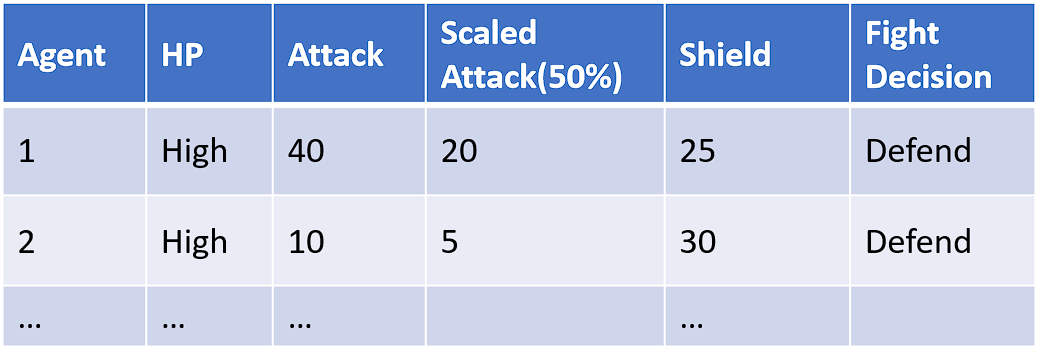
\includegraphics[width=0.6\textwidth]{008_team_5_agent_design/images/scaled-attack.PNG}
    \caption{Agent attack values are scaled by 50\%}
    \label{scaledattack}
\end{figure}

The scaling factors will give a more comprehensive view for different agent fight decision combinations, hence increasing our likelihood of finding a fight solution that is truly optimal. If all agents are alive, there could be up to 100 iterations for each of the 5 scaled attacks. But by performing each iteration in parallel, we can reduce the execution time and ensure time constraints are met.

If the number of fighting agents exceeds the calculated number of deaths for the iteration, the level is passed. From the iterations that meet this criterion, the one which optimises for least damage or least deaths are chosen with regards to our predetermined priority. The algorithm will finally return a fight decision map reflecting our best fight solution for the current level.

\subsection{Leader Allocation Logic}
By reasonably allocating loot pool resources the leader agent can benefit more agents without making any agent worse. In order to avoid Pareto inefficient, our agent will let anyone who requests the loot take their requested item, unless there is a clash. Our agent's duty is to solve the clash by iterating the fighting logic with the agents in the highest personality category, which also meet some extra conditions to enter iteration. This iteration is used to find where is the Pareto optimal that can utilise this item the most. The category of personalities and the rank of it, and extra conditions can be found in \ref{table:personality_impact}

\section{Fighting}
To pass the fighting game as an individual, we want our agent to have the ability to learn within a dynamic environment, where consequences could be introduced via an agent itself or other agents' actions. Learning in this case means to acquire a bank of knowledge and update them throughout time, in order to help fighting the monsters.

\subsection{Fight decision: Q learning}
The fighting stage from an individual agent's point could be viewed as a Markov Decision Process, where from the current state, an agent could have certain probability to transit into another state (new or same), by performing one of the three fighting actions, Attack / Defend / Cower. Depends on whether the agent end up in a better or worse state, it receive some corresponding reward which will cause it to like or dislike the action just being performed.

The state space is designed based on the health, stamina, attack and defence of an agent. Health and stamina are categorised relative to their initial value, so for agent with initial health of 1000, the \textit{Low} category is always $\leq 300$. However, the attack and defence are categorised relative to all other observable agents, for representing potential roles in a population. An agent could be a master fighter (\textit{Master}) when it's attack value is greater than most of the population, or it could be an elder or child (\textit{Weakee}) who's not that good at fighting.

\begin{table}[!ht]
    \centering
    \begin{tabular}{|l|l|l|l|}
        \hline
        \begin{tabular}[c]{@{}l@{}}Health \\ (to init health)\end{tabular}                      & \begin{tabular}[c]{@{}l@{}}Stamina \\ (to init stamina)\end{tabular}                    & \begin{tabular}[c]{@{}l@{}}Attack \\ (to observable agents)\end{tabular}                   & \begin{tabular}[c]{@{}l@{}}Defence \\ (to observable agents)\end{tabular}                  \\ \hline
        \textit{\begin{tabular}[c]{@{}l@{}}Low\\ hp \textless 30\%\end{tabular}}                & \textit{\begin{tabular}[c]{@{}l@{}}Low\\ ap \textless 30\%\end{tabular}}                & \textit{\begin{tabular}[c]{@{}l@{}}Weakee\\ AT \textless 25\%\end{tabular}}                & \textit{\begin{tabular}[c]{@{}l@{}}Weakee\\ SH \textless 25\%\end{tabular}}                \\ \hline
        \textit{\begin{tabular}[c]{@{}l@{}}Mid\\ 30\% \textless hp \textless 60\%\end{tabular}} & \textit{\begin{tabular}[c]{@{}l@{}}Mid\\ 30\% \textless ap \textless 60\%\end{tabular}} & \textit{\begin{tabular}[c]{@{}l@{}}Ordina\\ 25\% \textless AT \textless 75\%\end{tabular}} & \textit{\begin{tabular}[c]{@{}l@{}}Ordina\\ 25\% \textless SH \textless 75\%\end{tabular}} \\ \hline
        \textit{\begin{tabular}[c]{@{}l@{}}High\\ 60\% \textless hp\end{tabular}}               & \textit{\begin{tabular}[c]{@{}l@{}}High\\ 60\% \textless ap\end{tabular}}               & \textit{\begin{tabular}[c]{@{}l@{}}Master\\ 75\% \textless AT\end{tabular}}                & \textit{\begin{tabular}[c]{@{}l@{}}Master\\ 75\% \textless SH\end{tabular}}                \\ \hline
    \end{tabular}
\end{table}
\begin{figure}[!ht]
    \centering
    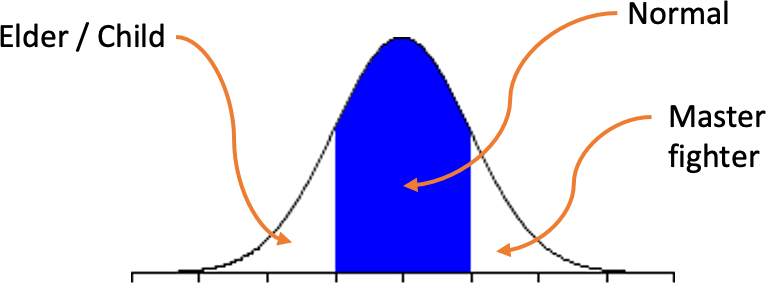
\includegraphics[width=0.6\textwidth]{008_team_5_agent_design/images/state_normal_distro.png}
    \caption{Assumed normal distribution of attack / defence roles.}
    \label{fig:state_normal_distro}
\end{figure}
\noindent
So in total there's 81 different states, where the health / stamina categories are equally separated; the attack / defence categories are separated assuming normal distribution, so extremes are less common and are valuable to treat differently.

In terms of decision, our agent utilise the Q learning algorithm, where each agent keeps a table of Q values as their utilities toward the fighting actions at a given state (a state-action pair), these Q values are updated throughout the game according to feedback (rewards) after each fighting round.

Updates rule:
\begin{center}
    $Q(S,A) \leftarrow Q(S,A) + \alpha(R(S^+) + \gamma \max\limits_{A^+} Q(S^+,A^+) - Q(S,A))$
\end{center}
\noindent
Where $Q(S,A)$ is the $Q$ value for a state($S$)-action($A$) pair; $R(S^+)$ is the reward received at the arrived new state, right now it's simply based on the percentage health loss / gain of an agent; $\gamma \max\limits_{A^+} Q(S^+,A^+)$ tries to reflect the potential future reward (in long term), propagate out with a decay rate $\gamma$; $\alpha$ is a learning rate determine how significant each update could be.

The key characteristics of Q learning is that it doesn't really need the state transition probabilities to solve a MDP; also it take in account of the long term effect of an action from a state by the $\gamma \max\limits_{A^+} Q(S^+,A^+)$ term.

Higher Q value for a state-action pair makes it more favourable for an agent to follow. So the strategy for an agent is to go for an action with the highest Q value at the current state, for exploiting its knowledge, but at the same time also allow some random deviation from that to explore the unknowns.

\subsection{Fight proposal: best self-experience}
As the exact opposite to making fight decision, which one has to answer the question ``what's the most promising action to do in such situation", making fight proposal to the others would be to answer the question ``what's the most promising situation to be in if one wants to conduct such action". So in our agent's case, it would be finding the state associated with the highest Q value for a given action.

\begin{figure}[!ht]
    \centering
    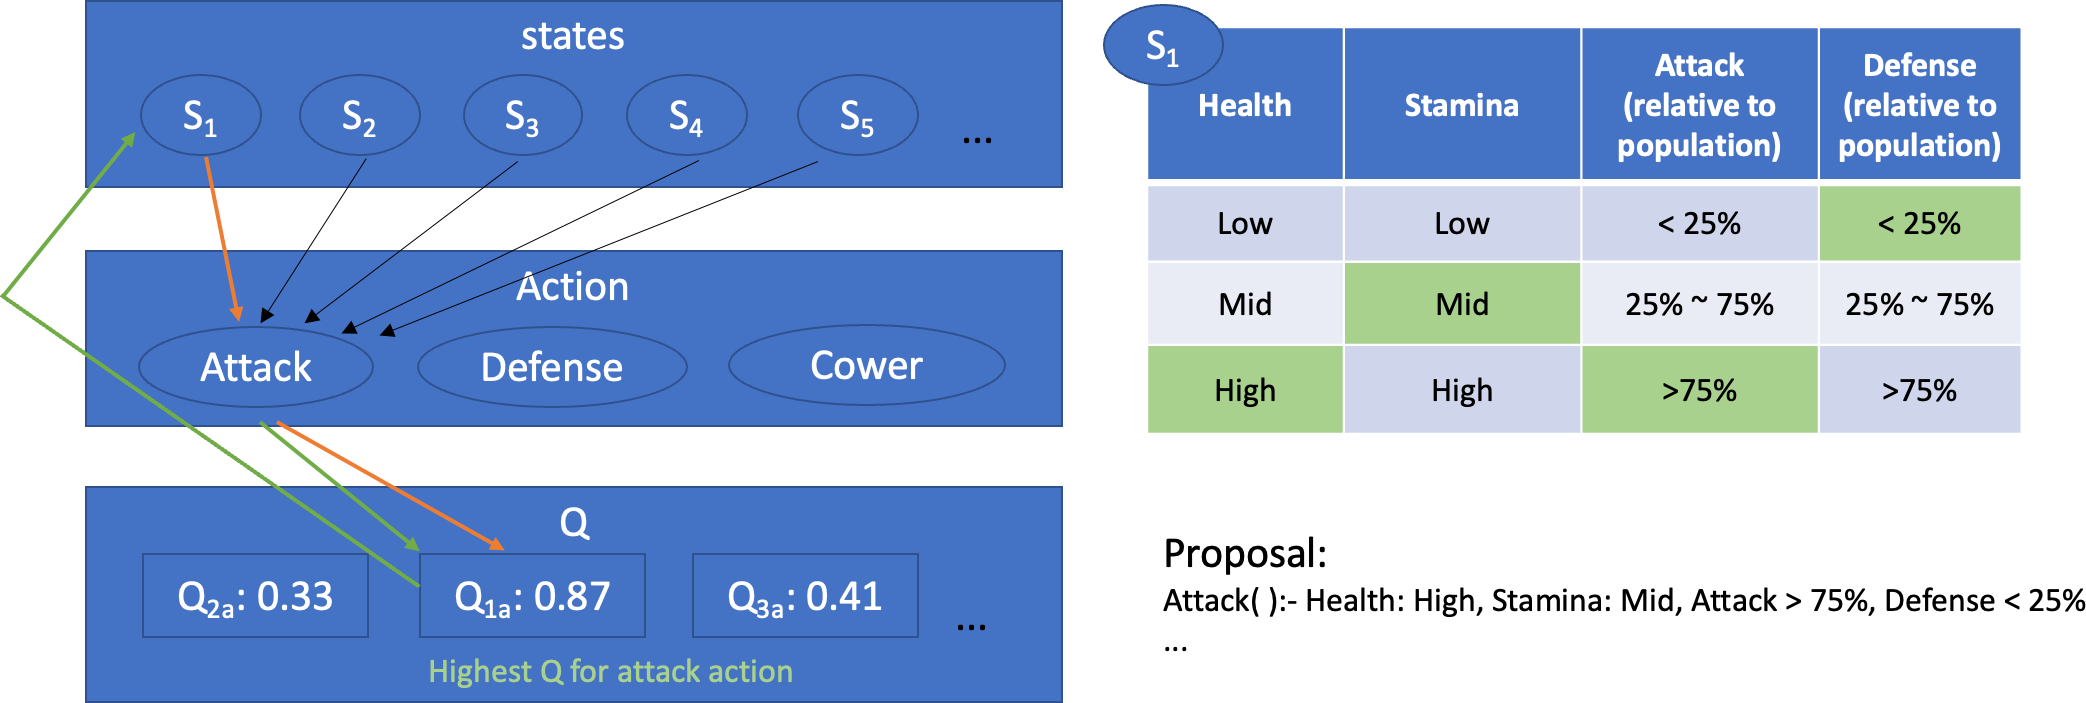
\includegraphics[width=1\textwidth]{008_team_5_agent_design/images/proposal_from_qtable.png}
    \caption{Proposing the most promising state for an action from the Q table}
    \label{fig:proposal_from_qtable}
\end{figure}

While every agent proposes the best strategy according to their self-experience, and all those proposals go to the leader, then depends on how the leader decided to board-cast the appropriate proposal(s) for the group, this could be seen as a process of trying to achieve knowledge aggregation.

\section{Election}
The election stage is setup so that, each of the $N$ agents need to vote for one or more of the other $N-1$ agents. Our agent is designed to produce a leading trust value $T_{lead}$ for every other agents, it aims to use this social capital to simplify the process of choosing the leader, without explicitly examining other's leader functions.

\subsection{Event-Recency dependent trust}
The trust is designed to be event and recency dependent, which means the recent event of an agent have more importance than those which are long time ago. More precisely defined as:

$$
    \qquad T(a,b) \leftarrow \gamma \cdot T(a,b) + v(r)
$$

Where $T(a,b)$ is the trust of agent $a$ toward agent $b$; $gamma$ is a decay factor to reduce the effect of past memory; $v(r)$ is the rating for an specific event $r$ that happened, typically related to health loss / gain of $a$ and death among the population.

The reason for making past memory become less important throughout time, is to avoid forming stereotype on leading strategies and to preserve diversity, accounting the possibility where one particular leading strategy might not be suitable at one time, but might be suitable for another time.

\subsection{Leader trust estimation}
Since it's not possible to get event feedback for how an agent is going to lead unless this agent is elected to be the leader, which tend to be infrequent, so we designed an estimation for the leader trust combining an agent's normal performance and it's performance when it did act as the leader.

$$
    T_{lead}^{t+1} = \alpha \cdot T_{lead}^t + \beta \cdot T_{normal}^t
$$

So in fact each agent need to keep two trust record for other agents, $T_{normal}$ for whether an agent is doing well on an individual level, and $T_{lead}$ for whether an agent is doing well on a group level. They are then combined to produce a estimation on how trust worthy an agent is to become the new leader, typically in a ratio of $\alpha=0.9, \beta=0.1$ for making past leading experience more significant.

\section{Trading}
\subsection{Trade Personality}

Our trade strategy extends the Agent's utilitarian approach and altruistic personality to achieving the collective aim. With this in mind, there is no significance in the weapon or shield we equip if the game is lost. Hence, no concern is given towards the weapon or shield equipped when finally escaping the pit. As each agent has an equal opportunity of receiving loot if they chose to fight, the exclusivity of shields and weapons are low. As we have no concern of our final equipped shield or weapon, the allocation of loot (consumption) to other agents will not subtract from our utility, deeming subtractability to be low. This in turn means that trading is not seen as a common pool resource problem.

On the contrary, other agents may value their weapon and shield equipped at the end of the game. In other words, trading will benefit other agents as weapon and shield statistics are valued, so the subtractability of weapons and shields would greatly increase in their perspective.

Considering agent's fight decision as their contribution towards loot, and by coupling trading with fight decision, we can frame this as a common pool resource problem. The common pool resource is sustained through defeating monsters with increasing difficulty to drop new and better items. Our agent takes advantage of this observation and rewards agents with regards to their contribution.

\begin{figure}[!ht]
    \centering
    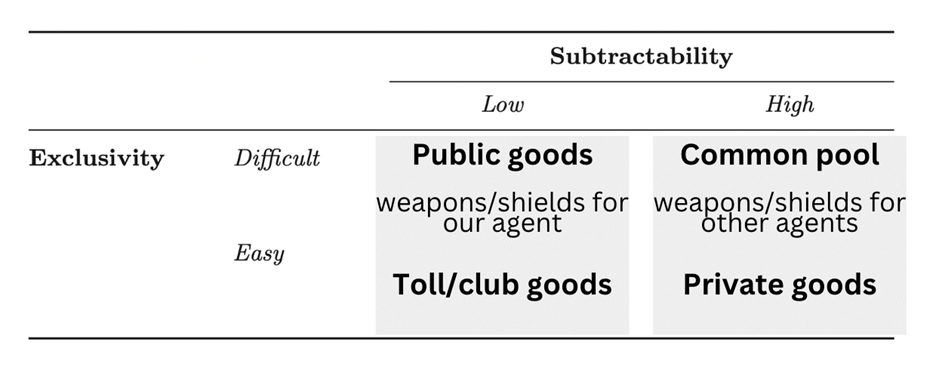
\includegraphics[width=0.60\textwidth]{008_team_5_agent_design/images/13.png}
    \caption{Our agent vs other agent's perspective on trading \cite{pitt}}
    \label{13}
\end{figure}

\subsection{Trade strategy}
Since each trading round is limited to five messages, choosing which agents to trade with is vital. The leader fight logic is used in our agent's trade strategy for every decision made. We use the outputted optimal fight decision map to filter out agents that will not likely fight in the following round. Agents predicted to either attack or defend will be prioritised as potential trade candidates. If our own agent is cowering for the following round, agents fighting will be offered our best weapon or shield. This is to ensure the best equipment are always utilised to maximise our chance to escape the pit and achieve the collective goal.

Our trading strategy will also prioritise agents having a positive or neutral strategy trust over agents with lower trust scores to penalise agents that either defected from their fight decision or are selfish in trades. The combination of agent trust and agent fight actions will reward and encourage agents to contribute towards the common pool resource.

An issue considered when choosing trade partners was if our policy was deterministic, such that our agent always requested from cowering agents with the best shield or weapon, all team 5 agents initialised within the game would have clashing trade requests. To resolve this issue, our agent searches for trade partners through random starting positions within the agent map and checks iteratively if agents meet our trade criteria of cowering and having a better weapon or shield. A trade request will sent to the first agent that meets our criteria.

\section{Experiment}

\subsection{Team 5 vs. Random}
Figure \ref{fig:Team5vsRandom} is a comparison between our team's agent vs. the random agent. With two small tweaks are done to the game engine in order to make the comparison under the same controls.

\begin{enumerate}
    \item Turned off HP pool donation: \\
          The current HP pool donation mechanism is way unbalanced and will become a dominated strategy if used, which causes agents to be able to skip all levels until they can't donate health anymore, this prevents all designs on fighting decision or leader function to be relevant.
    \item Stamina regeneration increased: \\
          As on the demo section, the unbalance stamina regeneration is mentioned, where after examining, the original game only regenerate 1 stamina ($0.05\%$ to initial health) per time, so for a more sensible game run, the stamina regeneration is changed to 100 ($5\%$ to initial health) per time.
\end{enumerate}

\begin{figure}[!ht]
    \centering
    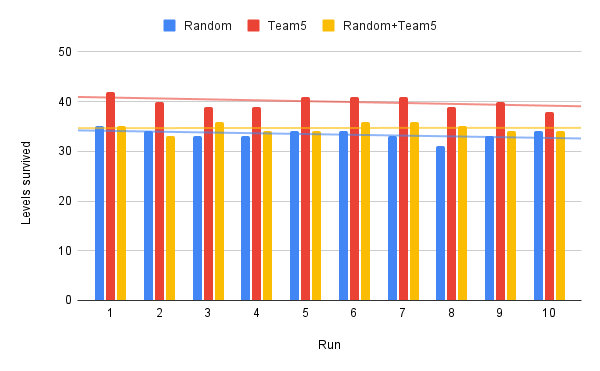
\includegraphics[width=0.8\textwidth]{008_team_5_agent_design/images/Team5vsRandom.png}
    \caption{Game run with 100 Team 5 agents (red); 100 Random agents (blue); 50 Team 5 agents and 50 Random agents (yellow).}
    \label{fig:Team5vsRandom}
\end{figure}

In average our agent could survive 5 more levels then the random agent, with it's own kind. But when playing with half of the population being another kind, the levels survived will only be marginally better than the random agents. This might because the random agents do not keep trust record (no social capital), so the advantage of using social capital to effectively elect leader or appropriating loot is broken.

\subsection{Social Network}

\begin{figure*}[!h]
    \subfloat[]{%
        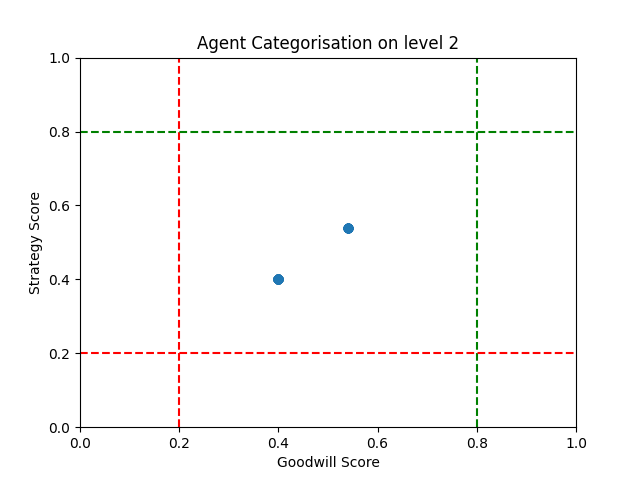
\includegraphics[width=.4\linewidth]{008_team_5_agent_design/images/level2.png}%
        \label{subfig:a}%
    }\hfill
    \subfloat[]{%
        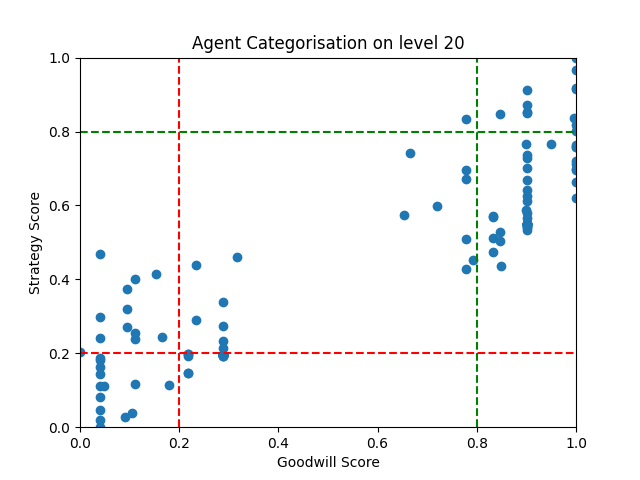
\includegraphics[width=.4\linewidth]{008_team_5_agent_design/images/level20.png}%
        \label{subfig:b}%
    }\\
    \subfloat[]{%
        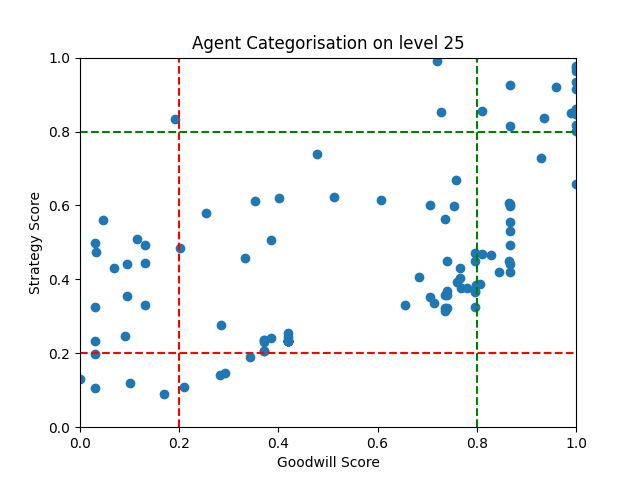
\includegraphics[width=.4\linewidth]{008_team_5_agent_design/images/level25.png}%
        \label{subfig:c}%
    }\hfill
    \subfloat[]{%
        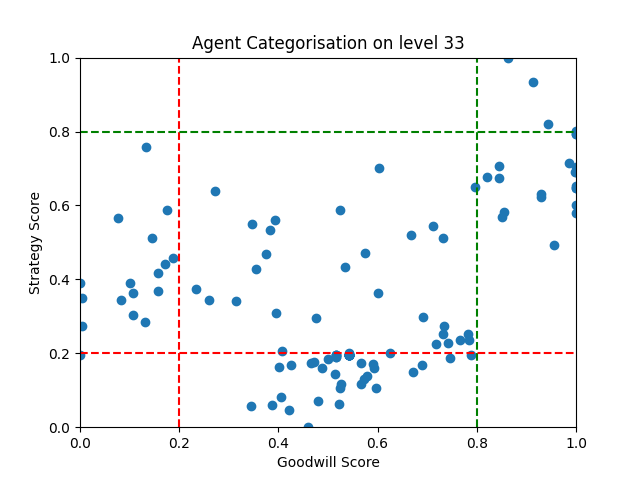
\includegraphics[width=.4\linewidth]{008_team_5_agent_design/images/level33.png}%
        \label{subfig:d}%
    }
    \caption{Agents' trust score at different levels, with strategy and goodwill personality boundaries both at 0.2 and 0.8, 30 of each type of agent are instantiated.}
    \label{fig:snRresults}
\end{figure*}

As the \ref{fig:snRresults} show, it appears that in a team5 agent's perspective, the system diverges and cliques up at around level 20. And then two due to the system being connected, the two cliques impact each other (level 25) and the two cliques dissolve into diverse places(level 33). The self-agent in an earlier stage of the game does not gain enough information to identify other agents' profiles. With more and more interactions and observations, the agent is able to identify smaller differences in other agents and separate them, which also involves scaling the scores in some of the updates.

\subsection{Leader Fight Logic}
The leader fight logic's execution time was tested to ensure it is within the time limit of 0.5 seconds.

\begin{figure}[htb]
    \centering
    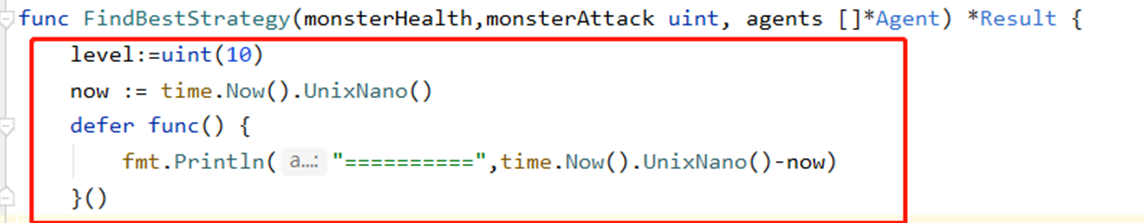
\includegraphics[width=0.7\textwidth]{008_team_5_agent_design/images/10.png}
    \caption{Measuring execution time}
    \label{testingexecutiontime}
\end{figure}

\begin{figure}[!ht]
    \centering
    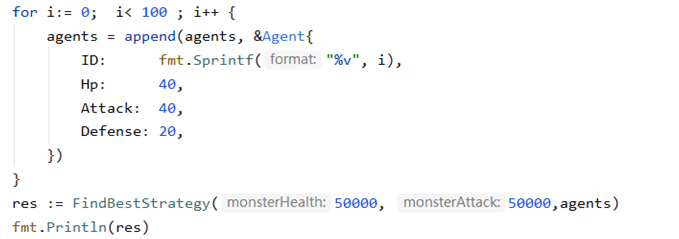
\includegraphics[width=0.7\textwidth]{008_team_5_agent_design/images/11.png}
    \caption{Initialising Agent and Monster}
    \label{initialisingagentandmonster}
\end{figure}

Some results are shown below, execution time is labelled with consumer in units of nano seconds.

\begin{figure}[!ht]
    \centering
    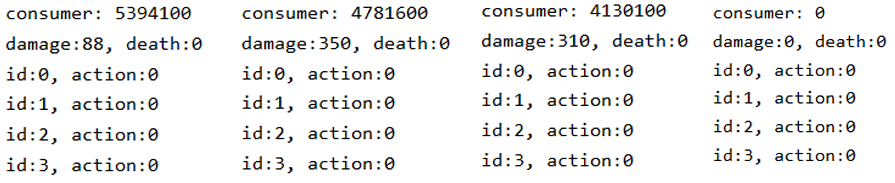
\includegraphics[width=0.7\textwidth]{008_team_5_agent_design/images/12.png}
    \caption{Execution time test results}
    \label{executiontimetestresults}
\end{figure}

All trials had execution time under 0.01 seconds and well below the time limit.

\subsection{Proposal, trust and knowledge aggregation}
It will be interesting to investigate the effect of allowing agents to propose what they think is the best, also how that might effect leading and whether it helps to do knowledge aggregation.

\begin{figure}[!ht]
    \centering
    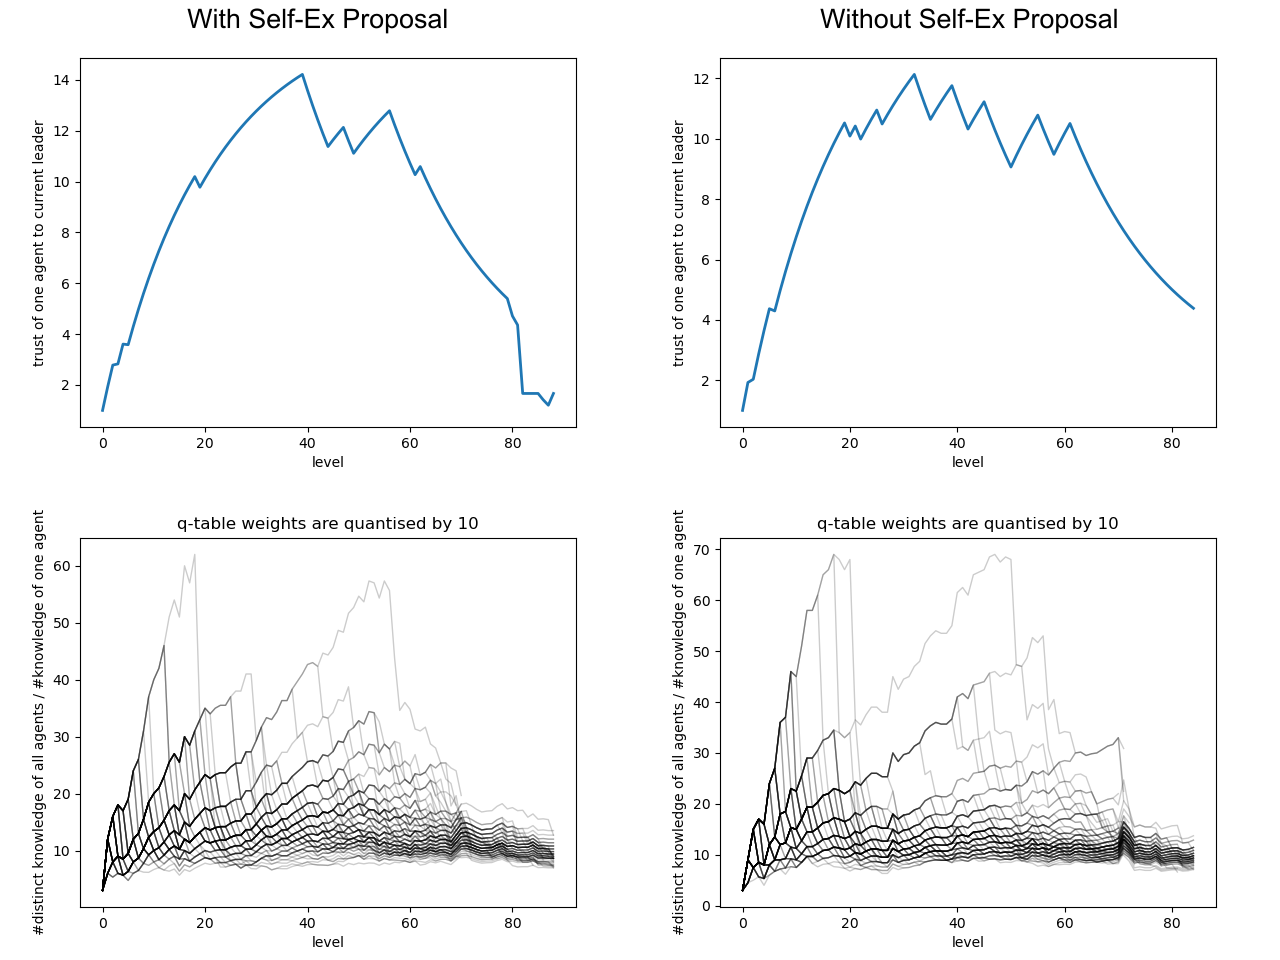
\includegraphics[width=0.8\textwidth]{008_team_5_agent_design/images/knowledgeAgg.png}
    \caption{Comparisons of allowing agent proposal or not. Top: agent's trust to the current leader through levels; Bottom: ratio of population knowledge to individual knowledge through levels.}
    \label{fig:knowledgeAgg}
\end{figure}
\pagebreak
For the top part of figure \ref{fig:knowledgeAgg}, we compared how proposal affects leading. Notice that without self-experience proposal, an agent's trust toward the current leader oscillates much frequently. This could infer more repeat leader change, also could be seen as an evidence for higher dependency on the leader.

For the bottom part of figure \ref{fig:knowledgeAgg}, we compared how proposal affects change of the population to individual knowledge ratio. In both cases, the ratio generally increases through the early part of the game, indicating the population knowledge base is growing in a much faster rate than each individual's, but start to drop at mid-game and finally converges. The one with proposal has more variations on how the ratio changes, resulting in more dense spaces between curves. This could reflect that the agents are trying to gain extract knowledge by accepting proposals from others.

\chapter{Team 6 Agent Design}\label{team_6_agent_design}

\section{Introduction}

Our agent has been designed to maximise both individual and collective ability. This has been achieved by maintaining four core beliefs:

\begin{itemize}
    \item Greed should be punished
    \item Irrationality should be punished
    \item Maintaining a team of semi-greedy, semi-rational agents is best for the collective
    \item Collective Intelligence and Group Think should be used under the right conditions
\end{itemize}
With these beliefs in mind, an overall strategy was devised:
\begin{itemize}
    \item Use a Social Capital system as the main driver for agent decision making
    \item Define a robust set of objectives for the Social Capital system
    \item Integrate learning into the system
\end{itemize}

\section{Social Capital System}

The main driver behind our agent's decision making is the Social Capital system. The system was designed with two key objective in mind - effectively managing finite common pool resources (avoiding the tragedy of the commons), and maximising self and collective utility. When combined, these improve the chance of escaping the pit. The system is also subject to three constraints - maximising agent state, obtaining a favourable loot distribution, and electing the most favourable leader.

To meet the requirements set out, five values are maintained for each agent in the game. The values are continuously updated as the game evolves. The values are:

\begin{itemize}
    \item Generosity (G)
    \item Bravery (B)
    \item Similarity (S)
    \item Leadership (L)
    \item Trust (T)
\end{itemize}

Each measure takes a value in the range [0,100] and is initialised to 50, with the exception of Bravery which is initialised to 100.

\subsection{Generosity}

\subsection{Bravery}

The Bravery value is used to track how often an agent either attacks or defends. The value itself is the proportion of rounds in which an agent fought or defended, rounded to the nearest integer. A value of 100 indicates that an agent never cowers, whereas a value of 0 indicates that an agent always cowers. This value aligns with the core belief that greed should be punished - not fighting is a form of greed, therefore an agent that doesn't fight is penalised.

The value is updated at the end of each level. Note that each level can consist of multiple fight rounds, therefore an agent's bravery value can change significantly.

\subsection{Similarity}

The Similarity value is used to track how closely another agents beliefs align with our own. This is achieved by comparing proposals (both loot and fight) with our own. It is believed that an agent's overall beliefs and strategy is well represented by their proposals, which makes this an attractive method for updating the value.

Whenever a proposal is received, either to vote on, or to be shared by us when we are the leader, equation \ref{eq:T6SimilarityFormula} is used to update the Similarity value for the proposer.

\begin{equation}\label{eq:T6SimilarityFormula}
    \begin{aligned}
    S_{i}=S_{i}+10(Sim(P_{i})-0.5) \\
    Sim(P) = \frac{1}{n}\sum_{k=1}^{n}f(P(A_{k}),P_{u}(A_{k})) \\
    f(D_{1},D_{2})=\left\{
    	\begin{array}{ll}
    		1 & \mbox{, if } D_{1} = D_{2} \\
    		0 & \mbox{, otherwise} 
    	\end{array}\right.
    \end{aligned}
\end{equation}
Where $S_{i}$ is the Similarity agent for the $i$th agent (the proposer), $P_{i}$ is the received proposal, $P_{u}$ is our own proposal, and $A_{1..n}$ is an array of predetermined agent states. The basic idea is to test both our own proposal and the received proposal on a range of agent states, and calculate the proportion of decisions (based on the agent states) that are equivalent when both proposals are applied. This gives a value in the range [0,1].

\subsection{Leadership}

There are three main factors that are considered when updating the Leadership value:

\begin{itemize}
    \item Freedom of Information - the leader should share proposals with the collective
    \item Change in agent state - the purpose of the leader is to improve the collective's success chances, therefore it is appropriate to judge the leader by the overall state of agents
    \item Responsibility - an agent shouldn't cower just because they are the leader, they should lead by example
\end{itemize}

Counts are maintained for the total number of proposals received, and the number of proposals received in the current round. At the end of each round, the leadership value is updated based on a comparison between the average number of proposals received per round, versus the number of proposals received in the current round. The relevant update is outlined by equation \ref{eq:T6LeadershipFOIFormula}.

\begin{equation}\label{eq:T6LeadershipFOIFormula}
    L_{L} = L_{L} + \frac{P_{c}-P_{a}}{4}
\end{equation}
Where $P_{c}$ is the number of proposals received in the current round, and $P_{a}$ is the average number of proposals received per round.

The final update occurs whenever a new leader is elected. The agent stores the Bravery value for the leader at the point of their appointment. At the end of their term, their current Bravery value is compared to the value at the start of their term. As the leader is expected to lead by example, any reduction in Bravery is punished, and any increase is rewarded. Equation \ref{eq:T6LeadershipBravery} outlines the process.

\begin{equation}\label{eq:T6LeadershipBravery}
    L_{L} = L_{L} + Max(-5,Min((B_{L}^{t}-B_{L}^{t-}),5))
\end{equation}
Where $B_{L}^{t-}$ is the leader's Bravery at the start of their term, and $B_{L}^{t}$ is the corresponding value at the end of their term.

\subsection{Trust}

The Trust value is a measure of how dependable other agents are. If an agent is told to take a certain action by the leader, do they comply or defect? At the end of each level a list of defectors is published by the game. All agents on this list have their Trust value decreased as per equation \ref{eq:T6TrustFormula}. Complying agents have their value increased.

\begin{equation}\label{eq:T6TrustFormula}
    T_{i}=\left\{
    	\begin{array}{ll}
    		T_{i}-10 & \mbox{, if agent i is on defector list} \\
    		T_{i}+2  & \mbox{, otherwise} 
    	\end{array}\right.
\end{equation}
Where $T_{i}$ is the Trust value for the $i$th agent.

If an agent defects, it takes 5 rounds of compliance to recover its initial trust value. This allows our agent to forgive those agents that only occasionally defect. Serial offenders will clearly be severely punished.

\section{Fighting}

\subsection{Fight Decisions}

The agent has its own internal rules for when it should attack, defend, and cower. These rules are based on the agent's state relative to its initial state. For example, if HP, Stamina, and Attack are all above the relevant thresholds, our agent will choose to attack. In the instances where the agent isn't given a proposed action, it will follow its own internal rules. If the agent is told what course of action to take, it follows this unless the internal rules tell it to cower and the proposal doesn't, in which case the agent will defect and cower. It is believed that the agent is in the best position to decide whether or not it should cower, as it has the best visibility of its own state.

\subsection{Fight Proposals}\label{T6FightProposals}

Our agent generates a fight proposal each round. This includes a number of rules based on an agent's state, and the fight action that should be taken if the condition is met. This proposal is sent to the leader 10\% of the time.
Proposals received are compared to our own proposal, using the $Sim$ function from equation \ref{eq:T6SimilarityFormula}. If the similarity score is $\geq 0.8$, the agent votes \textbf{for} the proposal, else the agent votes \textbf{against} the proposal.

\section{Loot}

\subsection{Loot Distribution Decisions}

\subsection{Loot Proposals}

All logic here is almost identical to \ref{T6FightProposals}. Only an agent's `needs' can be used to decide the loot distribution with the current proposal implementation. Therefore our agent generates its own proposal, sends it to the leader 10\% of the time, and uses similarity when voting on received proposals.

\subsection{Trading}

Trading is an essential part of the game, and if used properly can be very beneficial to the collective. Our trading strategy strikes a balance between selfishness and selflessness, so as to maximise both individual and collective utility. Each agent can be involved in multiple trade negotiations at once.
If our agent is not currently involved in a trade negotiation:

\begin{itemize}
    \item Determine if we want a weapon or shield (whichever is currently lower)
    \item Find an agent with a better version of that item (can iterate over agent states)
    \item Open a trade negotiation with that agent, offering the best item we wouldn't be using after the trade
\end{itemize}
When our agent receives incoming trade requests:

\begin{itemize}
    \item Accept any gifts (we can use these in later trades even if we don't use the weapon/shield)
    \item Decline any trades we can't partake in (don't have an item to satisfy the other agent)
    \item Accept if the agent is worse off than us and we can help without hindering ourselves (e.g. if they want a shield and our second best shield is better than their best shield, offer our second best shield)
    \item Accept if after the trade the sum of our Bonus Attack and Bonus Defense is greater than it was before the trade
    \item Accept if we really like the other agent (weighted sum of Social Capital values $\geq 0.8$)
    \item Decline in all other instances
\end{itemize}

This strategy allows us to improve our individual utility, increase other's utility without affecting our own, and to help agents we hold in high regard in times of need. This balanced approach ensures all agents should have access to the highest rated weapons and shields if they need them, and also allows us to prevent bad actors from hoarding items.

\section{Leadership}

\subsection{Running for Leader}\label{T6RunningForLeader}

Currently the game requires all agents to submit a leadership manifesto whenever a new leader needs to be appointed. Our agent has an initial idea of what a good manifesto looks like (`good' in this sense means both advantageous to the collective, and also likely to be viewed favourably by other agents). This initial manifesto is:

\begin{itemize}
    \item Not holding the loot decision power
    \item Not holding the fight decision power
    \item Term length of 3 levels
    \item Overthrow threshold of 51\% for no confidence votes
\end{itemize}

Our agent appreciates that its initial guess might not be great, so the manifesto dynamically changes as the game progresses. This is to both increase the likelihood of being selected, and for the benefit of the collective. The agent maintains an opinion for both the loot and fight decision powers. These opinions are in the range [0,100], where $>50$ means \textbf{should} have the power, and $\leq 50$ means \textbf{should not} have the power. Both values are initialised to 25, indicating that the agent believes it shouldn't hold either power as leader.

Values are also stored for term length and overthrow threshold. These are both floating point numbers to allow for fine tuning. All values are updated as per equation \ref{eq:T6ManifestoFormula}, and then restricted to an appropriate range (e.g. [1,10] for term length).

\begin{equation}\label{eq:T6ManifestoFormula}
    V_{u} = V_{u} + (L_{i}-50)*(V_{L}-V_{u}/100)
\end{equation}

Where $V_{u}$ is our agents value for a given manifesto element, $V_{L}$ is the value the previous leader was elected with (in the case of power values, this takes value 0 or 100), and $L_{i}$ is the outgoing leader's Leadership value. The same update is performed to all four elements of the election manifesto.

Manifesto creation involves updating the manifesto values, converting the power values to concrete decisions, and sending the manifesto to be voted on.

\subsection{Fight Decisions}

Our initial manifesto does not give our agent the power to overrule fight decisions. However, that manifesto can change, as outlined in \ref{T6RunningForLeader}, such that it is possible for our agent to be elected with the power to overrule fight decisions. One of our agent's beliefs is that freedom of information is to the advantage of the collective. Therefore, a reasonable proportions of fight proposals received as leader should be made available to all other agents. Once again, proposal similarity is used in this decision making. A similarity score is generated by the `Sim' function in equation \ref{eq:T6SimilarityFormula}, and if this value is $>0.6$ then the proposal is shared. This allows us as leader to influence the fight without appearing dictatorial. Once a proposal has been voted for, the proposed actions are sent to each agent unchanged, respecting the democratic outcome. Any agents that don't agree with the proposed action always have the opportunity to defect.

\subsection{Loot Decisions}

Logic for loot decisions is much the same as it was for fight decisions. This includes broadcasting any proposals that are more than 60\% similar to our own. Rescher \cite{rescher1966} introduces the concept of the `canons of distributive justice', which are derived from seven ways of treating people:

\begin{enumerate}
    \item ``as equals
    \item according to their needs
    \item according to their ability or merit or achievements
    \item according to their efforts and sacrifices
    \item according to their actual productive contribution
    \item according to the requirements of the common good, or the public interest, or the welfare of mankind, or the greater good of a greater number
    \item according to a valuation of their socially useful services in terms of supply and demand" \cite{rescher1966}
\end{enumerate}

The canons are to be considered in a given context, and `legitimate claims' established. In the context of the game and our Social Capital system, four canons were identified as related to `legitimate claims':

\begin{enumerate}
    \item The canon of Need
    \item The canon of Productivity
    \item The canon of Social Utility
    \item The canon of Supply and Demand
\end{enumerate}

\section{Elections}

\subsection{Leadership Elections}

Votes in leadership elections are critical for two main reasons:
\begin{enumerate}
    \item The leader can wield significant power
    \item Very few votes are required for a leader to be elected
\end{enumerate}
It is therefore of the utmost importance that our agent votes for a `good' leader. The following algorithm is used to vote:
\begin{enumerate}
    \item Generate a manifesto score
    \item Generate an opinion of the agent (weighted average of Social Capital values)
    \item Overall score = manifesto score * opinion
    \item Rank candidates according to overall score
    \item Vote for the highest ranked candidate (in case of plurality vote)
\end{enumerate}
The manifesto score is a value in the range [0,1], where 1 indicates that the manifesto is identical to our own. The score tends to 0 as a manifesto increasingly deviates from our own. The score is calculated according to equation \ref{eq:T6ManifestoScore}.

\begin{equation}\label{eq:T6ManifestoScore}
    M_{i}=\left\{
    	\begin{array}{ll}
    		0 & \mbox{, if } TL > 10 \mbox{ or } OT > 75 \\
    	  \sum_{k=1}^{4}\frac{1}{4+\left | U_{k} - C_{k} \right |} & \mbox{, otherwise} 
    	\end{array}\right.
\end{equation}
Where $TL$ is the manifesto's term length, $OT$ is the manifesto's overthrow threshold, $U_k$ is our value for 
the $k$th manifesto element, and $C_k$ is the corresponding value from the candidate's manifesto.

Equation \ref{eq:T6LeadershipOpinion} is used to calculate the opinion score.

\begin{equation}\label{eq:T6LeadershipOpinion}
    O_{i}=\left\{
    	\begin{array}{ll}
    		0 & \mbox{, if } L_{i} < 40 \\
    	  0.5 * L_{i} + 0.2 * S_{i} + 0.15 * T_{i} + 0.1 * B_{i} + 0.05 * G_{i} & \mbox{, otherwise} 
    	\end{array}\right.
\end{equation}
Where all variables are the social capital values for the $i$th agent (the candidate).

Once both scores have been calculated, the overall score can be derived (see equation \ref{eq:T6OverallLeadershipFormula}).

\begin{equation}\label{eq:T6OverallLeadershipFormula}
    R_{i} = M_{i} * O_{i}
\end{equation}

All candidates are ranked based on their score $R_{i}$, and in the case of plurality voting the top ranked candidate is chosen. If Borda count is used, all agents with a score $\geq 0.5$ are put on the ballot. If no agents meet this threshold, the agent votes for itself.

\subsection{No Confidence Votes}

For no confidence votes, a combination of Social Capital values and objective success are used to determine our vote. In this instance objective success refers to the number of agents that died in the most recent round.

Much like in leadership elections, an overall opinion of the leader is derived from their social capital values, as per equation \ref{eq:T6NoConfidenceOpinionFormula}. This is then multiplied by a scaling factor, giving a final measure of the leader's performance (equation \ref{eq:T6AgentDeathsFormula} and equation \ref{eq:T6NoConfidenceValue}).

\begin{equation}\label{eq:T6NoConfidenceOpinionFormula}
    O_{L} = 0.5 * L_{L} + 0.2 * S_{L} + 0.15 * T_{L} + 0.1 * B_{L} + 0.05 * G_{L}
\end{equation}

\begin{equation}\label{eq:T6AgentDeathsFormula}
    \delta = \frac{1}{1+0.25*AD}
\end{equation}
Where $AD$ is the number of agent deaths in the most recent round.

\begin{equation}\label{eq:T6NoConfidenceValue}
    N_{L} = \delta * O_{L} 
\end{equation}
If $N_{L} > 55$ vote `positive', else if $N_L < 45$ vote `negative', else `abstain' as the agent has no strong opinion either way.

\section{HP Pool Donation}

\section{Collective Intelligence and Group think}
\subsection{Collective Intelligence}
In so far, most decision-making will be shaped by each agent's individual beliefs, ie. their social capital system. However, in such a collective community, it is important to note that knowledge is distributed amongst all agents. As such, even though each agent may believe they are making the most rational decision, this is based on the fact that, in most cases, the decision being made is informed by the information and knowledge available to the agent at the time when the decision was made.

However, should this agent access the information and knowledge held by other agents, it is likely that they may be able to make more rational decisions, hence maximizing their utility, within their self-defined social capital system.

Representative of our society, this game has introduced the concept of distributed knowledge by adding a level of anonymity to each agent state, such as the health of each agent being only accessible in discrete levels or not being able to access information regarding other agents' inventory.

This introduces the idea of collective intelligence, where given that knowledge is distributed, the  individuals should share their knowledge, data, and skills such that through collaboration and communication, it should be possible to maximize collective utility.\\

\subsubsection{Communication}
In many cases, it may not be possible to do this. In such a time and resource-limited environment facing imminent danger, the cost of this communication could be too high. In other cases, it may not even be possible. Alternatively, some agents will, through their social capital values, choose to not participate in any collaboration or communication. This game environment also reproduces some of these limitations which force agents to be a little creative - What system can be used which can capitalise on collective intelligence with minimal communication, dispute resolution, and computational cost? \\
As a result, there must be a way in which each agent should implicitly be able to observe other agents and make informed decisions, on whether an agent may have some information, not available to them, which they can use to maximize their self-utility.

\subsection{Group Think}
This behaviour can be observed in nature. Consider the picture below showing a shoal of fish. 

The use of this `collective intelligence informed group think' also tackles imbalance within decision-making and can under the right conditions enrich the democratic system in place.

\section{Experiments}

\section{Future Improvements}

\chapter{Experiments}\label{experiments}

\input{011_results/011_results}
\chapter{Discussion}\label{sec:discussion}

\section{Reflection}

Ultimately, this project was interesting, challenging, and very teaching, and there is a great deal we as a class can learn from this experience. When beginning this undertaking, many of us were very involved and excited about how to best self organize and accomplish this task. However, there were many who took much longer to organize into teams, voice their opinions, and show that they understood the facets of the course, leading to delays in the process of building out our game. In retrospect, there seem to have been misunderstandings regarding what exactly was expected of us. An example of this is our proposal of utilizing a force fight imposition and forgoing disobedience, rather than focusing on institutionalized power and sanctions in response to disobedience. As such, we should have set clearly defined goals regarding what we wanted to achieve in designing this game, and how each facet of this related to what we learned in the course. One clear improvement we could have made, is better communication. We can categorize communication into two main types: communication of ideas that we want to see in the game, and communication of what has been implemented for the game. Regarding ideas, many of us seemed to have focused directly on the game during the early stages rather than the course. This led to individuals and teams realizing much later that their agent needed to incorporate more elements of what we learned rather than what we thought initially; however, this put a great degree of stress on the infrastructure team as it meant changing much of what had already been agreed upon. A clear solution to this is ensuring that members of each team understand what they are trying to accomplish from the beginning and making sure that they voice these ideas to the infrastructure and game design teams. One recommendation could be to implement some method of holding individuals accountable for their learning of the course material. This could be in the form of in-class quizzes, class-participation marks, or some other mandatory class involvement. The main logic behind this recommendation is because it seems many individuals from the start were more focused on their mark rather than the course material. As such, a method of ensuring a widespread understanding of course material from early on might allow more people to be better equipped to voice their opinions throughout the course rather than just at the end. Regarding the communication of implementation, many teams seemed to have a limited understanding of what exactly had been implemented and how they utilize these implementations. This was because of poor documentation, and subpar discussion between the infrastructure, game design, and individual agent teams. One improvement could be to ensure there are clear leaders from each team that give consistent updates regarding what has been designed or implemented and how people can use it when coming up with their own agents.  

Some other issues were present regarding the implementation of the infrastructure. As the messaging system did not work, teams were prevented from implementing agents that could get a strong idea of other agent's performance, and their reputations. This in turn impacted the amount of information that could be sent to the chair which ultimately prevented governance implementation from being as sophisticated as some teams planned. This seems to tie back to the issue of communication mentioned earlier. In retrospect, defining clear goals of what we wanted for the project, and why we wanted these goals achieved would be much more conducive to a project that emulates the facets of self organising multi-agent systems.
\chapter{Conclusion}\label{conclusion}

Each teams results show that the addition of social interactions between agents and informed collective decision making improve agent performance when compared to a population of agents acting purely randomly. However, it is also clear that a more comprehensive and wide ranging set of possible messages between agents would have greatly aided their decision making processes and allowed team to see the full influence of their ideologies. In conjunction with this, improved mathematics algorithms would make the game easier to analyse and play by spreading deaths over many levels, instead of mass deaths and quick end-games. 

Therefore this project concludes that the introduction of a norm-governed society, where agents interact on a social level to determine collective actions and allocate sparse resources, allowed the players to advance further in the game. Possible future developments would involve integrating all team agents into a single environment and see if the combination of different non-random agents improves performance. This would hinge upon a new agent communication language, expanding the messages agents can send to fully utilise their strategies.  

% teams could do better than random
% more communication subjects would further increase prgoresses
% better math algos w.r.t stamina potions would make the game easier and winnable

% future work... integrate the agents and develop a new agent comms language and see if the combination of no random agents improves the performance of the game 
% Appendix
\appendix
\chapter{Team 1 Appendix}

The following video\footnote{Requires Acrobat Reader to view} is an example of the type of visualisation developed to observe the relationship between input parameters and social capital, or the relationship between social capital and elements within the game (eg HP, elections).

\begin{figure}[!h]
\begin{frame}{}
  \centering
  \animategraphics[loop,controls,width=0.7\linewidth]{2}{004_team_1_agent_design/vid/graph}{1}{36}

\end{frame}
\caption{Video showing social capital values changing throughout a game}
  \label{ani:sc_visual_vid}
\end{figure}

% References
\newpage
\nocite{*}
\bibliography{references} 
\bibliographystyle{unsrtnat}

%%%%%%%%%%%%%%%%%%%%%%%%%%%%%%%%%%%%%%%%%%%%%%%%%%%%%%%%%%%%%%%%%
%                        Document End                           %
%%%%%%%%%%%%%%%%%%%%%%%%%%%%%%%%%%%%%%%%%%%%%%%%%%%%%%%%%%%%%%%%%
\end{document}
